%\documentclass[fleqn]{article}
\documentclass[msc,numbers, fleqn]{coppe}
\renewcommand\thesection{\arabic{section}}
\usepackage[utf8]{inputenc}
\usepackage{hyperref}
\usepackage{indentfirst}
\usepackage{empheq}
%\usepackage{mathptmx}
\usepackage{amsmath}
\usepackage{amssymb}
\usepackage{gensymb}
\usepackage{commath}
\usepackage{cancel}
\usepackage{tikz}
\usepackage{bm}
\usepackage{siunitx}
\usepackage{tcolorbox}
\usepackage{pgfplots}
\usepackage{filecontents}
\usepackage{natbib} 
\usepackage{graphicx}
\usepackage{setspace}
\usepackage[font=small, labelfont=bf]{caption}
\usepackage{enumerate}
\usepackage{nccmath}
\usepackage{booktabs}
\usepackage{multirow}
\usepackage{wasysym}
\usepackage{xcolor}
\usepackage{float}
%\usepackage{titlesec}
%\usepackage{kantlipsum}
\setcitestyle{authoryear,round, sort}
\usepackage[nottoc]{tocbibind}
%\captionsetup[figure]{font={stretch=1.5}}
\usetikzlibrary{shapes.geometric,calc}
\pgfplotsset{compat=1.4}
% \addtolength{\oddsidemargin}{-.875in}
% \addtolength{\evensidemargin}{-.875in}
% \addtolength{\textwidth}{1.75in}
% 
% \addtolength{\topmargin}{-.875in}
% \addtolength{\textheight}{1.75in}
\pgfplotsset{compat=newest} % Allows to place the legend below plot
\usepgfplotslibrary{units} % Allows to enter the units nicely
\renewcommand{\baselinestretch}{1.5}

\allowdisplaybreaks

\setcounter{secnumdepth}{5}

\numberwithin{figure}{section}
\numberwithin{table}{section}
\numberwithin{equation}{section}


\makelosymbols
\makeloabbreviations

\newcommand{\graficostemperatura}[5]{%
	\begin{minipage}[t][6cm][c]{4.5cm}
		\centering		
		\begin{tikzpicture}[scale=0.75]
		\begin{axis}[
		%/pgf/number format/1000 sep={.},/pgf/number format/use comma,
		axis lines=left,
		%		xmin = 0,
		%		xmax = 0.04,
		%ymin = #4,
		%ymax = #5,
		%		restrict y to domain=-500:2000,
		scaled x ticks = false,
		scaled y ticks = false,
		x tick label style={/pgf/number format/fixed},
		y tick label style={/pgf/number format/fixed},
		anchor=east,  
		width=7cm,
		height=5cm,
		label style={font=\footnotesize},
		xlabel = $x$(m),
		ylabel= $T_1\big|_{\Gamma_0}$ (\celsius),
		ylabel style={rotate=-90, at={(-0.1, 1)}, anchor = south west}]		
		\pgfplotstableread{../data/temperaturas_sinteticas_interface_0#1_conductance_0#2_stdev_05.dat} 
		\teff
		\addplot[only marks,color=gray,mark=triangle,mark options={mark size=2.0pt}] table from \teff;
		\pgfplotstableread{../data/temperaturas_sinteticas_interface_0#1_conductance_0#2_stdev_01.dat} 
		\teff
		\addplot[only marks,color=red,mark=square,mark options={mark size=2.0pt}] table from \teff;
		\pgfplotstableread{../data/temperaturas_sinteticas_interface_0#1_conductance_0#2_stdev_00.dat} 
		\teff
		\addplot[color=blue,mark=o,mark options={mark size=2.0pt}] table from \teff;		
		\end{axis}
		\end{tikzpicture}
		\caption*{(#3) Perfil #2}
	\end{minipage}
}%

% Parametros:
% erro_rms
% delta_temperatura ou fluxo_calor
% interface_id: 1, 2, ou 3
% condutance_id: 1, 2, ou 3
% axis text
% a, b, ou c
\newcommand{\graficoerrorms}[6]{%
	\begin{minipage}[t][6cm][c]{4.5cm}
		\centering		
		\begin{tikzpicture}[scale=0.75]
		\begin{axis}[
		axis lines=left,
		%/pgf/number format/1000 sep={.},/pgf/number format/use comma,
		%ymode = log,
		grid=major,
		legend style={legend pos=north west}
		% xmin = 0.00000001,
		%		xmax = 0.04,
		%ymin = 0,
		%ymax = 90,
		scaled x ticks = true,
		scaled y ticks = true,
		x tick label style={/pgf/number format/fixed},
		y tick label style={/pgf/number format/fixed},
		xtick = {0,5,10,15,20,25,30,35,40,45,50},
		anchor=east,  
		width=7cm,
		height=6cm,
		label style={font=\footnotesize},
		xlabel = $N_j$,
		ylabel= $\log\left(\delta_{#5}\right)$,
		ylabel style={rotate=-90, at={(-0.1, 1)}, anchor = south west}]
		\pgfplotstableread{../data/#1_#2_interface_0#3_conductance_0#4_stdev_00.dat} 
		\teff
		\addplot[color=blue,mark=o,mark options={mark size=2.0pt}] table from \teff;
		\pgfplotstableread{../data/#1_#2_interface_0#3_conductance_0#4_stdev_01.dat} 
		\teff
		\addplot[color=red,mark=square,mark options={mark size=2.0pt}] table from \teff;
		\pgfplotstableread{../data/#1_#2_interface_0#3_conductance_0#4_stdev_05.dat} 
		\teff
		\addplot[color=gray,mark=triangle,mark options={mark size=2.0pt}] table from \teff;
		\end{axis}
		\end{tikzpicture}
		\caption*{(#6)Perfil #4}
	\end{minipage}
}%

%Parametros
% delta_temperatura ou fluxo_calor
% interface_idx : 1, 2, ou 3
% condutance_idx : 1, 2, ou 3
% numero de autofunces para cada desvio padrao, com dois algarismos
% a, b, ou c
\newcommand{\graficoestimativa}[9]{%
	\begin{minipage}[c][3cm][c]{0.3\textwidth}
		\centering		
		\begin{tikzpicture}[scale=0.65]
		\begin{axis}[
		axis lines=left,
		%/pgf/number format/1000 sep={.},/pgf/number format/use comma,
		%		xmin = 0,
		%		xmax = 0.04,
		%		ymin = 310,
		%		ymax = 340,
		%		restrict y to domain=-500:2000,
		scaled x ticks = false,
		scaled y ticks = false,
		x tick label style={/pgf/number format/fixed},
		y tick label style={/pgf/number format/fixed},
		anchor=east,  
		width=5cm,
		height=4cm,
		label style={font=\footnotesize},
		xlabel = $x$(m),
		ylabel= $#8$ (#9),
		ylabel style={rotate=-90, at={(-0.1, 1)}, anchor = south west}]
		\pgfplotstableread{../data/comsol/#1_interface_0#2_conductance_0#3.dat} 
		\teff
		\addplot[color=black, line width=1.5pt] table from \teff;
		\pgfplotstableread{../data/fortran/#1_interface_0#2_conductance_0#3_stdev_00_N_#4.dat} 
		\teff
		\addplot[only marks, color=blue,mark=o,mark options={mark size=1.5pt}] table from \teff;
		\pgfplotstableread{../data/fortran/#1_interface_0#2_conductance_0#3_stdev_01_N_#5.dat} 
		\teff
		\addplot[only marks,color=red,mark=square,mark options={mark size=1.5pt}] table from \teff;
		\pgfplotstableread{../data/fortran/#1_interface_0#2_conductance_0#3_stdev_05_N_#6.dat} 
		\teff
		\addplot[only marks,color=gray,mark=triangle,mark options={mark size=1.5pt}] table from \teff;
		\end{axis}
		\end{tikzpicture}
		%\caption*{(#7) Perfil #3}
	\end{minipage}
}%

\newcommand{\graficoctc}[4]{%
	\begin{minipage}[t][3cm][c]{0.3\textwidth}
		\centering		
		\begin{tikzpicture}[scale=0.65]
		\begin{axis}[
		axis lines=left,
		%/pgf/number format/1000 sep={.},/pgf/number format/use comma,
		%		xmin = 0,
		%		xmax = 0.04,
		%		ymin = 310,
		%		ymax = 340,
		%		restrict y to domain=-500:2000,
		scaled x ticks = false,
		scaled y ticks = false,
		x tick label style={/pgf/number format/fixed},
		y tick label style={/pgf/number format/fixed},
		anchor=east,  
		width=5cm,
		height=4cm,
		label style={font=\footnotesize},
		xlabel = $x$(m),
		ylabel= $h_c$ (W/$\text{m}^2$\celsius),
		ylabel style={rotate=-90, at={(-0.1, 1)}, anchor = south west}]
		\pgfplotstableread{../data/conductance_#2.dat} 
		\teff
		\addplot[color=black, line width=1.5pt] table from \teff;
		\pgfplotstableread{../data/estimativa_ctc_interface_#1_conductance_#2_stdev_00.dat} 
		\teff
		\addplot[only marks, color=blue,mark=o,mark options={mark size=1.5pt}] table from \teff;
		\pgfplotstableread{../data/estimativa_ctc_interface_#1_conductance_#2_stdev_01.dat} 
		\teff
		\addplot[only marks,color=red,mark=square,mark options={mark size=1.5pt}] table from \teff;
		\pgfplotstableread{../data/estimativa_ctc_interface_#1_conductance_#2_stdev_05.dat} 
		\teff
		\addplot[only marks,color=gray,mark=triangle,mark options={mark size=1.5pt}] table from \teff;
		\end{axis}
		\end{tikzpicture}
		%\caption*{(#4) Perfil #3}
	\end{minipage}
}%

\newcommand{\graficosmetricas}[4]{%
	\begin{minipage}[t][6cm][c]{4.5cm}
	\centering		
	\begin{tikzpicture}[scale=0.75]
	\begin{axis}[
	%/pgf/number format/1000 sep={.},/pgf/number format/use comma,
	axis lines=left,
	ymode = log,
	scaled x ticks = false,
	scaled y ticks = false,
	x tick label style={/pgf/number format/fixed},
	y tick label style={/pgf/number format/fixed},
	anchor=east,  
	width=7cm,
	height=5cm,
	label style={font=\footnotesize},
	xlabel = $x$(m),
	ylabel= $T_1\big|_{\Gamma_0}$ (\celsius),
	ylabel style={rotate=-90, at={(-0.1, 1)}, anchor = south west}]			
	\addplot[color=blue,mark=triangle,mark options={mark size=2.0pt}] table[x index=0,y index=#4] {../data/erro_rms_interface_0#1_conductance_0#2_stdev_0#3.dat};				
	\end{axis}
	\end{tikzpicture}
	%\caption*{(#3) Perfil #2}
	\end{minipage}
}%

\newcommand{\graficointerface}[1]{%
	\begin{minipage}[c][2cm][c]{\textwidth}
	\centering
	\begin{tikzpicture}[scale=0.5]
	\begin{axis}[
	anchor=east,  
	ticks=none,
	width=6cm,
	height=3cm,
	%ylabel=Iterações Lineares,
	xmin = 0,
	xmax = 0.04,
	ymin = 0,
	ymax = 0.02]
	\pgfplotstableread{../data/interface_0#1.dat} 
	\teff
	\addplot[color=blue,mark=none,smooth] table from \teff;
	\end{axis}			
	\end{tikzpicture}	
	\end{minipage}
}%

\newcommand{\graficosctclegenda}{%
	\begin{minipage}[c][2cm][c]{0.3\textwidth}
	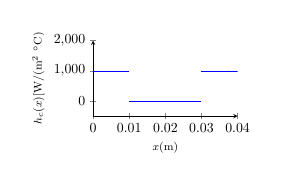
\begin{tikzpicture}[scale=0.5]
	\begin{axis}[
	%/pgf/number format/1000 sep={.},/pgf/number format/use comma,
	axis lines=left,
	xmin = 0,
	xmax = 0.04,
	ymin = -500,
	ymax = 2000,
	restrict y to domain=-500:2000,
	scaled x ticks = false,
	scaled y ticks = false,
	x tick label style={/pgf/number format/fixed},
	y tick label style={/pgf/number format/fixed},
	anchor=east,  
	width=5.25cm,
	height=3.5cm,
	label style={font=\footnotesize},
	xlabel = $x$(m),
	ylabel= $h_c(x)[$W/($\text{m}^2$ \celsius)]]
	\addplot[color=blue,mark=none,smooth, domain=0:0.01] {1000};
	\addplot[color=blue,mark=none,smooth, domain=0.01:0.03] {0};
	\addplot[color=blue,mark=none,smooth, domain=0.03:0.04] {1000};
	\end{axis}			
	\end{tikzpicture}	
	\end{minipage}
	\begin{minipage}[c][2cm][c]{0.3\textwidth}
	\begin{tikzpicture}[scale=0.5]
	\begin{axis}[
	%/pgf/number format/1000 sep={.},/pgf/number format/use comma,
	axis lines=left,
	xmin = 0,
	xmax = 0.04,
	ymin = -500,
	ymax = 2000,
	restrict y to domain=-500:2000,
	scaled x ticks = false,
	scaled y ticks = false,
	x tick label style={/pgf/number format/fixed},
	y tick label style={/pgf/number format/fixed},
	anchor=east,  
	width=5.25cm,
	height=3.5cm,
	label style={font=\footnotesize},
	xlabel = $x$(m),
	ylabel= $h_c(x)$[W/($\text{m}^2$ \celsius)]]
	\pgfplotstableread{../data/conductance_02.dat} 
	\teff
	\addplot[color=blue,mark=none,smooth] table from \teff;
	\end{axis}			
	\end{tikzpicture}	
	\end{minipage}
	\begin{minipage}[c][2cm][c]{0.3\textwidth}
	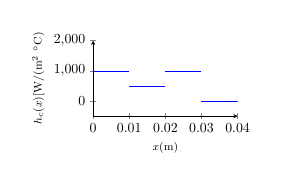
\begin{tikzpicture}[scale=0.5]
	\begin{axis}[
	%/pgf/number format/1000 sep={.},/pgf/number format/use comma,
	axis lines=left,
	xmin = 0,
	xmax = 0.04,
	ymin = -500,
	ymax = 2000,
	restrict y to domain=-500:2000,
	scaled x ticks = false,
	scaled y ticks = false,
	x tick label style={/pgf/number format/fixed},
	y tick label style={/pgf/number format/fixed},
	anchor=east,  
	width=5.25cm,
	height=3.5cm,
	label style={font=\footnotesize},
	xlabel = $x$(m),
	ylabel= $h_c(x)$[W/($\text{m}^2$ \celsius)]]
	\addplot[color=blue,mark=none,smooth, domain=0:0.01] {1000};
	\addplot[color=blue,mark=none,smooth, domain=0.01:0.02] {500};
	\addplot[color=blue,mark=none,smooth, domain=0.02:0.03] {1000};
	\addplot[color=blue,mark=none,smooth, domain=0.03:0.04] {0};
	\end{axis}	
	\end{tikzpicture}	
	\end{minipage}
}%

\newcommand{\legendagraficos}{%
	\caption{$\text{--} \rightarrow \text{Exato}$; $\textcolor{blue}{\ocircle} \rightarrow \sigma = 0.0\celsius$; $\textcolor{red}{\square} \rightarrow \sigma = 0.1\celsius$; $\textcolor{gray}{\triangle} \rightarrow \sigma = 0.5 \celsius$}	
}%


\begin{document}

\abbrev{SI}{Sistema Internacional de Unidades}
\abbrev{RTC}{Resistência térmica de contato}
\abbrev{CTC}{Condutância térmica de contato}
\abbrev{IHTP}{\textit{Inverse Heat Transfer Problem} -- Problema Inverso de Transferência de Calor}

\symbl{$\mathbb{R}$}{Conjunto dos n\'umeros reais}

\title{Estimativa
de condutâncias térmicas de contato em interfaces irregulares usando a
técnica da Transformada Integral Clássica e o método dos funcionais de reciprocidade}
\foreigntitle{Estimation of thermal contact conductances on irregular interfaces using the generalized integral transform technique
and the reciprocity functional method}
  \author{Guilherme}{Camelo de Freitas}
  \advisor{Prof.}{Marcelo José}{Colaço}{D.Sc.}
  \examiner{Prof.}{Marcelo José Colaço}{D.Sc.}
  \examiner{Prof.}{Helcio Rangel Barreto Orlande}{Ph.D.}
  %\examiner{Prof.}{Manuel Ernani de Carvalho Cruz}{Ph.D.}
  \examiner{Prof.}{Nilson Costa Roberty}{D.Sc.}
  \examiner{Prof.}{Luiz Alberto da Silva Abreu}{D.Sc.}
  \department{PEM}
  \date{\month}{\the\year}
  
  \keyword{Problemas Inversos}
  \keyword{Funcional de Reciprocidade}
  \keyword{Condutância Térmica de Contato}
  \keyword{Transformada Integral}
 
 \maketitle
 
 \frontmatter
  \dedication{À Ludmilla, minha esposa, minha companheira, minha amiga, minha âncora. Te amo!}
  
  \chapter*{Agradecimentos}
  
  Agradeço a Deus, pois em todo tempo é bom.
  
  À Petrobras, pela oportunidade oferecida.
  
  À minha esposa Ludmilla, que sempre esteve ao meu lado em todo esse processo. Dedico este trabalho a você.

  Ao meu gerente imediato, Roberto Gonçalves, por proporcionar condições adequadas que permitiram a conclusão deste trabalho.
  
  Ao professor Marcelo Colaço, pela orientação e paciência, e sobretudo pela confiança.
  
  Ao professor Renato Cotta, que me apresentou a técnica da Transformação Integral Clássica.
  
  Aos meus colegas de trabalho e amigos Daniel Fialho e Andreia Carvalho, pelo apoio e compreensão durante o período de desenvolvimento deste trabalho.
  
  Ao meu colega de trabalho e amigo Elísio Caetano Filho, pelo incentivo a não desistir.
  
  Aos meus colegas de trabalho e amigos Eduardo Gaspari, Carlos Dittz e Ricardo Minette, pelas sugestões e trocas de ideias.
  

 
 \begin{abstract}
 
O método dos funcionais de reciprocidade, aliado à Técnica da Transformada Integral Clássica (CITT), tem sido aplicado com sucesso na obtenção de
soluções analíticas para o problema inverso de transferência de calor que procura estimar a distribuição da condutância térmica de contato (CTC) ao longo da interface plana
de um corpo constituído de dois materiais. O desenvolvimento teórico sobre o qual esta abordagem se baseia, contudo, não está limitado à necessidade de que esta
interface tenha um formato regular.

Este trabalho propõe estender o método, obtendo assim um desenvolvimento analítico para estimativa da distribuição da condutância térmica de contato em interfaces não necessariamente
regulares. Para tanto, algumas ferramentas serão empregadas, a saber: a extensão do domínio físico irregular num domínio físico regular sobre o qual os
problemas auxiliares serão resolvidos analiticamente; e a aplicação do processo de ortogonalização de Gram-Schmidt para gerar um conjunto ortonormal
de funções a partir das soluções obtidas pelos problemas auxiliares.

Vários problemas-teste foram resolvidos usando as técnicas descritas neste trabalho, levando a resultados muito bons, com baixo uso de tempo de CPU por parte da implementação computacional. O efeito na qualidade das estimativas devido à presença de erros de medição nos dados de entrada também foi analisado.


  \end{abstract}
  
  \begin{foreignabstract}

The reciprocity functional method, associated to the Classic Integral Transform Technique (CITT), has been succesfully applied in obtaining analytical
solutions for the inverse heat transfer problem that seeks to estimate the thermal contact conductance (TCC) distribution on the interface of a body composed of
two materials. Yet, the theoretical development upon which this approach is based is not limited to the need of this interface to have a regular format.

This work proposes to extend the method, thus obtaining an analytical development for the estimation of the thermal contact conductance distribution on interfaces which
are not necessarily regular. Therefore, some tools will be employed, namely: the extension of the irregular physical domain to a regular physical domain in
which the auxiliary problems will be analytically solved; and the application of the Gram-Schmidt orthogonalization process in order to generate an orthonormal set
of functions from the solutions obtained from the auxiliary problems.

Several test problems were solved using the techniques described in this work, leading to very good results, with low CPU time usage by the computational implementation. The effect on the quality of the estimates due to the presence of measurement errors in the input data was also analyzed.
 
  \end{foreignabstract}

\tableofcontents
 \listoffigures
 \listoftables
 \printlosymbols
 \printloabbreviations

  \mainmatter
  
\section{Introdução}

\subsection{Motivação}

Quando há transferência de calor através da fronteira comum entre dois corpos materiais em contato físico, observa-se experimentalmente que nessa interface há
uma descontinuidade no perfil de temperatura, ou seja, o contato térmico nessa região não é perfeito \citep{livro_ozisik}. 
Esse fenômeno ocorre devido à combinação dos efeitos de três componentes \citep{livro_madhusudana}:
\begin{itemize}
  \item Condução de calor através dos pontos em que há contato efetivo sólido-sólido, devido à presença de irregularidades microscópicas e macroscópicas;
  \item Condução de calor através do meio intersticial, preenchido por algum fluido (por exemplo, ar) ou vácuo;
  \item Radiação de calor, que é desprezada na maioria das aplicações. 
\end{itemize} 


% 
% Na maioria das aplicações, os efeitos de radiação são desprezados, bem como  Mesmo a altas pressões, o fenômeno da descontinuidade de temperatura permanece relevante, pois a
% superfície efetiva de contato não coincide com a superfície total de contato.

A figura \ref{fig1} ilustra o processo de transferência de calor através da interface de contato entre dois sólidos. As linhas de fluxo de calor
sofrem uma \textit{constrição} nos pontos de contato; nos espaços entre os pontos, devido às dimensões das lacunas da ordem de micrômetros, a convecção
de calor é desconsiderada em detrimento da condução.

\begin{figure}[h!b]
\begin{center}
\begin{tikzpicture}
\node at (0, 0)
	{
		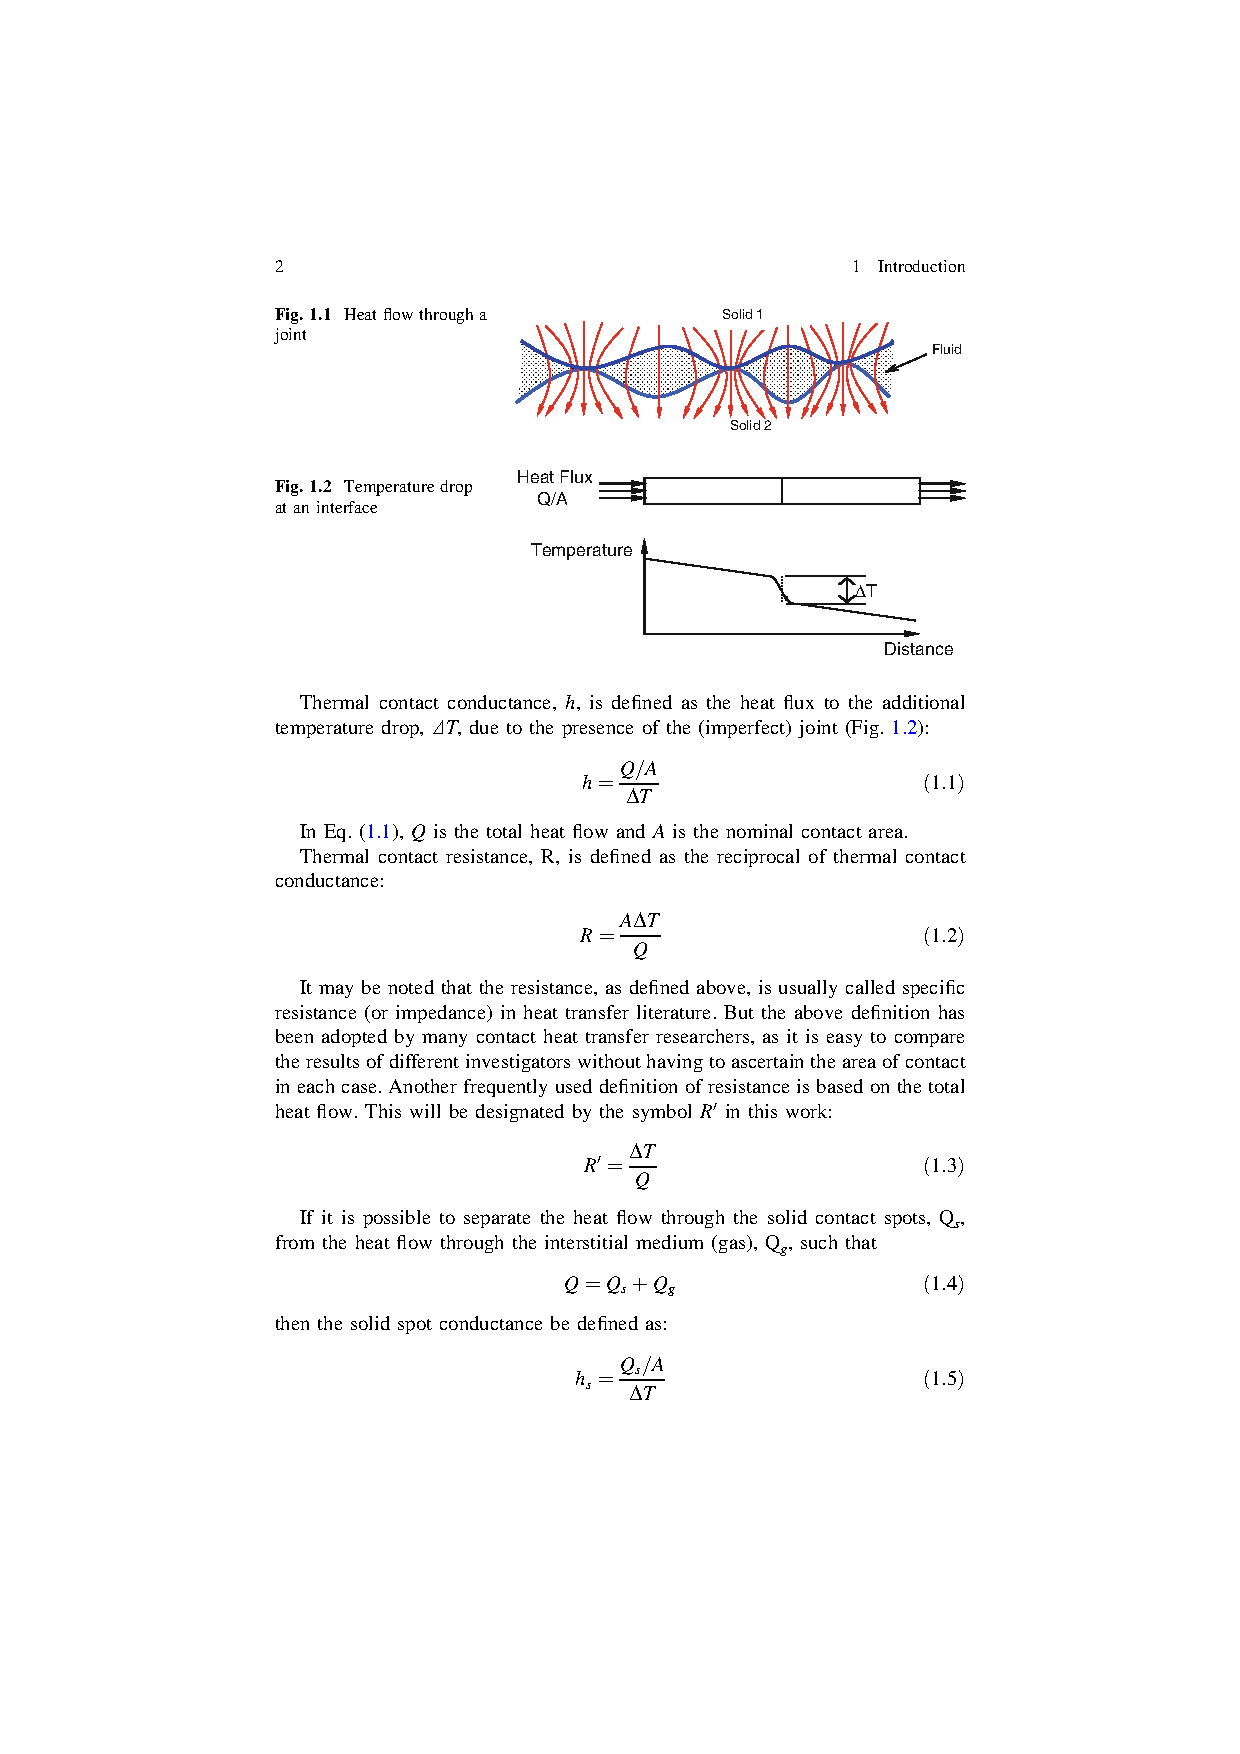
\includegraphics[trim=250 642 150 154, clip=true]{img/img1.pdf}
	};
	
\node[scale=0.8] at (0, 0.9) {Sólido 1};
\node[scale=0.8] at (0, -1.1) {Sólido 2};
\node[scale=0.8] at (4, 0.3) {Fluido};
\end{tikzpicture}
\caption{Transferência de calor através da interface entre dois corpos (adaptado de \citeauthor{livro_ozisik}, \citeyear{livro_ozisik})}
\label{fig1}
\end{center}
\end{figure}

A \textit{condutância térmica de contato} -- abreviada como CTC -- é definida como sendo a razão entre o fluxo de calor e o salto de temperatura
devido à presença do contato imperfeito \citep{livro_madhusudana}:
\begin{equation}
	h_c = \frac{Q_c/A}{\Delta T_c} = \frac{q_c}{\Delta T_c} \label{eq:definicao_1}
\end{equation}
onde $Q_C$ é o fluxo total de calor através da interface, $A$ é a área de contato nominal ou aparente, $q_c$ é o fluxo de calor por unidade de área e e $\Delta T_c$ é o salto de temperatura na interface. As unidades
da CTC são as mesmas do coeficiente de transferência de calor por convecção ($W/m^2 K$ no SI).

A inversa da CTC é denominada \textit{resistência térmica de contato} (RTC):
\begin{equation}
	R_c = \frac{1}{h_c} = \frac{A\Delta T_c}{Q_c} = \frac{\Delta T_c}{q_c}
\end{equation}

Uma definição equivalente da CTC pode ser formulada a partir da análise do problema de condução de calor no domínio constituído pelos
corpos em contato, através das condições de contorno avaliadas na interface de contato \citep{livro_ozisik}. Nessa região, pode-se afirmar que o fluxo
de calor saindo ou entrando em cada um dos sólidos deve se igualar ao fluxo de calor através da interface.

Sejam, portanto, $T_1$ e $T_2$ os campos de temperatura em cada um dos sólidos cuja interface é representada na figura \ref{fig1}. Sejam $k_1$ e $k_2$
as respectivas condutividades térmicas dos sólidos, e seja $q_c$ o fluxo de calor por unidade de área através da interface de contato. Assim, o balanço de energia permite escrever:
\begin{equation}
	q_c = -k_1\frac{\partial T_1}{\partial \mathbf{n}_1}\bigg|_i
	=
	h_c(T_1 - T_2)_i
	=
	k_2\frac{\partial T_2}{\partial \mathbf{n}_2}\bigg|_i \label{eq:definicao_2}
\end{equation}
De onde se obtém:
\begin{equation}
	h_c = \frac{-k_1\displaystyle\frac{\partial T_1}{\partial \mathbf{n}_1}\bigg|_i}{(T_1 - T_2)_i} = \frac{k_2\displaystyle\frac{\partial T_2}{\partial \mathbf{n}_2}\bigg|_i}{(T_1 - T_2)_i} \label{eq:definicao_3}
\end{equation}
Os gradientes de temperatura são calculados sobre as direções dos vetores normais
$\mathbf{n}_1$ e $\mathbf{n}_2$, que apontam para fora das fronteiras que delimitam os corpos materiais correspondentes; em particular,
na interface de contato teremos $\mathbf{n}_2 = -\mathbf{n}_1$. O subscrito $i$ indica que todas as avaliações são feitas sobre a superfície de contato.

Nota-se facilmente a partir da equação \eqref{eq:definicao_3} que a CTC é uma propriedade não necessariamente constante ao longo da interface de contato,
uma vez que tanto o fluxo de calor como o salto entre as temperaturas podem variar em cada ponto sobre a interface. De fato, nos locais onde a diferença é nula (ou seja, o contato
é perfeito), a CTC assumiria valor infinito, ou alternativamente, a RTC seria nula. No outro extremo, havendo uma região micrométrica perfeitamente
isolante entre os corpos materiais, o fluxo de calor seria nulo para uma diferença de temperatura finita; ali a CTC seria nula, equivalente a um valor
infinito de RTC. Assim, a CTC também pode ser entendida como um parâmetro de avaliação da qualidade do contato entre dois corpos materiais.

O levantamento da CTC também permite avaliar qualitativamente a presença de descontinuidades ou falhas
em materiais homogêneos, uma vez que, devido aos saltos de temperatura provocados pela interface de contato no local da falha,
o campo de temperatura medido na superfície externa fornece resultados diferentes do esperado se tais falhas não ocorressem.

A necessidade de cálculo ou estimativa da CTC se faz presente em diversas aplicações, como por exemplo, na área aeroespacial \citep{artigo_aerospacial}, microeletrônica
\citep{artigo_snaith}, ou no projeto de trocadores de calor \citep{artigo_huang}. Para tanto, podem ser aplicados métodos de medição que normalmente exigem
algum conhecimento de detalhes das superfícies de contato, tais como rugosidade ou aspereza, e necessitam de tomadas de temperatura no interior dos corpos em contato, levando a arranjos
experimentais complexos ou intrusivos. Conhecidas (ou estimadas por regressão) as temperaturas na interface e o fluxo de calor por unidade de área, a aplicação
direta da definição permite levantar a CTC, normalmente como um valor médio sobre a interface. Essa foi a abordagem adotada na maioria dos problemas de estimativa
de CTC registrados na literatura.

O problema da estimativa da CTC tem características que permitem classificá-lo como um problema inverso de transferência de calor (IHTP, do termo em inglês
\textit{Inverse Heat Transfer Problem}). Num problema direto de transferência de calor, conhecem-se as propriedades termofísicas dos materiais envolvidos,
a taxa de geração de calor e as
condições de contorno e inicial; através desses parâmetros se obtém a distribuição de temperaturas no domínio de interesse. Já o problema inverso procura
estimar algum dos parâmetros relacionados previamente, utilizando medidas de temperatura em um ou mais pontos do domínio \citep{livro_beck_2}.
Nesse contexto, a CTC se enquadra como um parâmetro termofísico passível de ser estimado através da resolução de um IHTP. Uma grande vantagem dessa
abordagem é a possibilidade de tratar a CTC como um parâmetro distribuído espacialmente ao longo da interface de contato; por outro lado, problemas
inversos são bastante sensíveis a erros de medição dos parâmetros de entrada. Algumas estratégias podem ser aplicadas
a fim de contornar essas dificuldades, como por exemplo a técnica de regularização de Tikhonov \citep{livro_tikonov}.

O tratamento da estimativa da CTC como um problema inverso de transferência de calor não eliminou a necessidade de se ter disponíveis as medições de
temperatura na interface de contato. A determinação indireta da distribuição dessas temperaturas sobre a interface, através de métodos não intrusivos,
tem sido objeto de pesquisas recentes, levando ao desenvolvimento de técnicas de estimativa de CTC mais precisas e mais eficientes computacionalmente
\citep{artigo_colaco_1, artigo_colaco_2, artigo_colaco_3, artigo_colaco_4, artigo_padilha_3}. Tais técnicas, porém, têm sido aplicadas em configurações
físicas e geométricas regulares, tais como interfaces de contato planas ou de seção transversal circular, o que simplifica consideravelmente o tratamento
analítico-numérico do problema inverso de transferência de calor, em detrimento de uma maior abrangência em resolver problemas de estimativa de CTC
envolvendo geometrias menos comuns.

\subsection{Objetivo}

O objetivo principal desta dissertação é, através de uma abordagem analítico-numérica, estudar o problema da estimativa da CTC entre superfícies
de dois corpos materiais colocados em contato, considerando o fato de que tais superfícies não são necessariamente regulares.  

O ponto de partida foi o trabalho desenvolvido por \cite{tese_padilha}, que estudou o problema da estimativa da CTC numa superfície
plana entre dois corpos materiais colocados em contato. O problema-teste analisado foi configurado de forma que a seção transversal do
conjunto composto pelos dois
corpos materiais tivesse formato retangular e a CTC sobre a interface dependesse
espacialmente de apenas uma coordenada cartesiana. O referido trabalho forneceu uma expressão analítica que estima de forma direta
o perfil de CTC ao longo do comprimento da interface. Para resolução do problema inverso que fornecia a CTC, foram empregadas as técnicas dos Funcionais de Reciprocidade \citep{artigo_andrieux},
e da Transformação Integral Clássica (CITT) \citep{livro_cotta}. Este resultado representou uma contribuição inédita aos estudos de levantamento de perfil de CTC,
ao introduzir um método direto, não iterativo, de baixo custo computacional e que não emprega medidas intrusivas de temperatura no interior dos corpos em contato.

Ao se acompanhar o desenvolvimento analítico envolvendo o uso da técnica dos Funcionais de Reciprocidade, nota-se que as expressões obtidas, basicamente integrais de contorno, não dependiam necessariamente de
alguma geometria particular de seção transversal dos corpos materiais, ou da interface de contato, ou mesmo do sistema de coordenadas empregado.
Contudo, as características geométricas do problema-teste original permitiram que o emprego da CITT simplificasse consideravelmente estas integrais.

Para desenvolver esta dissertação, foi feita uma modificação na configuração geométrica do problema-teste: a interface de contato entre os corpos passou a
ter uma forma curvilínea, representada por uma equação da forma $y = w(x)$, mantendo-se o formato retangular na seção transversal do conjunto
de teste. Assim, a interface plana estudada por \cite{tese_padilha} passou a ser um caso particular do problema abordado no presente trabalho, para
o qual $w(x) = \text{constante}$. Essa alteração introduziu complexidades ao problema que, num primeiro momento, eliminariam as vantagens computacionais
proporcionadas pelo emprego da CITT, e que foram contornadas através do uso de conceitos e ferramentas clássicas da Álgebra Linear e de uma redefinição conveniente
do domínio geométrico do problema.

\subsection{Organização do trabalho}

O presente capítulo introduziu a definição formal de condutância térmica de contato e apresentou os conceitos e ferramentas básicas a serem aplicados ao longo do trabalho (a saber, os Funcionais de Reciprocidade e a Técnica da Transformada Integral Clássica). Os fatores motivacionais e os objetivos principais da dissertação também foram apresentados.

No capítulo 2 é apresentada uma revisão bibliográfica descrevendo separadamente a evolução das técnicas de solução de problemas difusivos e as abordagens do tratamento da estimativa da condutância térmica de contato. O problema matemático necessário para o cálculo dos Funcionais de Reciprocidade é basicamente um problema difusivo, para o qual existem diversas opções de técnicas de solução; já os primeiros problemas de determinação da condutância térmica de contato não eram entendidos como problemas inversos de condução de calor (que são difusivos por definição). Ambos aspectos são citados e desenvolvidos pelo ponto de vista histórico neste capítulo.

O capítulo 3 apresenta a descrição do problema físico abordado neste estudo. A configuração física, que consiste basicamente em um corpo de prova de seção reta retangular feito de dois materias distintos em contato, foi estabelecida levando-se em conta que a interface de contato entre os materiais pode ser representada por uma curva. As hipóteses assumidas e a formulação matemática do problema de condução de calor, em que a CTC aparece como um dos parâmetros de entrada, são indicados neste capítulo.

O capítulo 4 descreve o problema inverso de condução de calor referente ao arranjo físico estabelecido no capítulo 3, no qual a CTC passa a ser um parâmetro a ser estimado. Neste arranjo, assume-se que as medidas de temperatura na superfície superior do corpo de prova são conhecidas. O conceito de Funcional de Reciprocidade é descrito neste capítulo, bem como a sua formulação proposta para o problema estudado. Conceitos matemáticos de Álgebra Linear necessários para o embasamento teórico da técnica dos Funcionais de Reciprocidade, tais como espaços lineares, produtos internos e projeções ortogonais, também são discutidos.

No capítulo 5 são formulados os problemas difusivos auxiliares que fornecem as funções auxiliares necessárias para o cálculo dos Funcionais de Reciprocidade. Uma vez que a interface de contato entre os materiais que compõem o corpo de prova não é plana nem horizontal, faz-se necessário aplicar conceitos de Geometria Diferencial para expressar em coordenadas cartesianas o gradiente de temperatura ao longo da interface, que aparece nas condições de contorno dos problemas auxiliares. Desse modo, é feita uma adequação da formulação dos problemas para permitir a aplicação da Técnica da Transformada Integral Clássica para sua solução; todo o processo de resolução através desta ferramenta é detalhado neste capítulo. As funções obtidas são então ortogonalizadas através do algoritmo de Gram-Schmidt.

Os resultados obtidos nos capítulos anteriores são reunidos no capítulo 6, onde finalmente é apresentada a formulação analítica da estimativa da condutância térmica de contato. Mais uma vez são revisitadas ferramentas de Geometria Diferencial, quais sejam, integrais de linha e derivadas direcionais, que auxiliam na formalização das conceitos estabelecidos ao longo do trablho. A expressão final proposta é de propósito geral, para interfaces de contato de formato arbitrário, sendo a interface plana horizontal, que inspirou o presente trabalho, um caso particular.

Discussões sobre a implementação numérico-computacional da estimativa da condutância térmica de contato têm lugar no capítulo 7. Foram executadas simulações computacionais de diferentes configurações de geometria de interface de contato e de condutância térmica de contato, a fim de obter as medidas simuladas de temperatura na superfície superior dos corpos de prova. Estas medidas por sua vez alimentaram um programa escrito em Fortran, que implementa as equações deduzidas até o capítulo anterior, fornecendo as respectivas estimativas de condutância térmica de contato. Os resultados teóricos e estimados foram comparados e as análises correspondentes foram desenvolvidas ao longo deste capítulo.

A dissertação se encerra no capítulo 8, onde são apresentadas conclusões quanto ao emprego da técnica dos Funcionais de Reciprocidade no problema inverso estudado e indica sugestões de trabalhos futuros para a continuidade do desenvolvimento desta técnica.

\section{Revisão bibliográfica}

A revisão bibliográfica exposta neste capítulo está dividida em duas partes. Na primeira parte, é feito um levantamento sobre a evolução histórica
das técnicas de solução de problemas difusivos, uma vez que, conforme será visto nos próximos capítulos, o problema inverso de condução de calor
a partir do qual será estimada a CTC é um problema difusivo. Na segunda parte, é apresentado um apanhado dos trabalhos clássicos que envolvem o tema da
determinação da CTC, antes e depois da introdução da abordagem deste tema como um problema inverso.

\subsection{Técnicas de soluções de problemas difusivos}

Segundo \cite{livro_tanehill}, há basicamente três abordagens ou métodos que podem ser usados para resolver um problema
de mecânica dos fluidos e/ou transferência de calor: experimental, teórico (ou analítico) e computacional (ou numérico). O primeiro
fornece resultados mais realistas a um custo de implementação maior. Já o segundo faz suposições
simplificadoras a fim de facilitar o tratamento do problema, e possivelmente encontrar uma solução fechada, ou seja, que é expressa geralmente como uma fórmula
matemática; uma vez que não envolve iterações ou interpolações, a obtenção do valor da solução num determinado ponto do domínio é praticamente imediata,
com baixo custo computacional. No último método -- a abordagem numérica -- as equações que governam o fenômeno em estudo são substituídas por
esquemas numéricos, cuja solução (obtida através de cálculos manuais ou pelo emprego de computadores digitais) é usada para representar de forma
aproximada a solução do problema original.

A teoria matemática moderna sobre a condução de calor foi estabelecida por Joseph Fourier, que reuniu suas investigações teóricas em sua obra
\textit{Théorie analytique de la chaleur} \citep{livro_fourier, artigo_langer}. Neste trabalho, Fourier deduz analiticamente as equações de condução para vários
tipos de sólidos, como esferas, prismas retangulares ou cilindros de seção reta circular. Nesses problemas, o fluxo de calor tinha
sempre uma direção que favorecia o aspecto simétrico do sólido em questão; por exemplo, no caso do cilindro ou da esfera, o fluxo
de calor acontecia na direção radial. Em seguida, Fourier apresenta a formulação tridimensional em coordenadas cartesianas da equação
de condução de calor em regime transiente, e a emprega para levantar as equações obtidas previamente, através de substituições de
variáveis. Finalmente, Fourier desenvolve o conceito de representação de uma função como um somatório infinito de funções
trigonométricas\footnote{A história registra que, quando Fourier apresentou seus artigos sobre a representação de funções arbitrárias
como expansões de senos e cossenos à Academia de Ciências de Paris em 1807 e 1811, recebeu críticas dos consultores (principalmente Lagrange,
que negou veementemente essa possibilidade), devido à falta de rigor, e por isso os artigos não foram publicados \citep{livro_agarwal}.} e, através da aplicação
da técnica de separação de variáveis, usa esse conceito na resolução analítica dos problemas que propôs no início do trabalho. Uma vez que os domínios envolvidos e as
condições de contorno impostas nos problemas possuíam algum tipo de simetria, que simplificava a variação da temperatura para apenas uma
variável dimensional (distância radial, comprimento ao longo de um eixo, etc.), as soluções encontradas eram relativamente simples, o que não
diminui sua importância por modelarem matematicamente o fenômeno físico da condução de calor pela primeira vez. O tratamento
dado por Fourier aos problemas de condução de calor foi, em suma, predominantemente analítico, sem considerações de caráter numérico.

Historicamente, os livros acadêmicos que versam sobre transferência de calor reproduzem a dedução da equação de condução em coordenadas
cartesianas feita por Fourier e em seguida apresentam a formulação equivalente nos sistemas de coordenadas cilíndricas e esféricas; ver
por exemplo \cite{livro_carslaw}, \cite{livro_holman} e \cite{livro_ozisik}. Em tese, a formulação no sistema cartesiano é aplicável
a qualquer tipo de geometria; a solução geral sempre poderá ser expressa em termos de somatórios de senos ou cossenos. Soluções analíticas obtidas
nos sistemas de coordenadas esféricas ou cilíndricas envolvem somatórios de tipos diferentes de funções base ortogonais, obtidas através da aplicação do método
de separação de variáveis \citep{livro_boyce}. Voltando a citar os trabalhos de Fourier, em que são feitas análises do problema de condução de calor em corpos cilíndricos ou esféricos, as equações correspondentes são expressas nos sistemas de coordenadas cilíndricas ou esféricas, para as quais são esboçadas soluções em forma de séries \citep{livro_fourier}. 

\cite{artigo_einsenhart, artigo_einsenhart_2} demonstrou que a equação de Helmholtz (da qual a equação
de difusão é um caso particular) pode ser resolvida por separação de variáveis em onze diferentes
sistemas de coordenadas ortogonais, dentre as quais figuram os sistemas cartesiano, esférico e cilíndrico, bem como outros menos usuais, tais
como elíptico-cilíndrico ou parabólico. \cite{livro_moon} fizeram um extenso levantamento das equações diferenciais ordinárias
oriundas da separação de variáveis em cada um desses sistemas, e apresentam suas respectivas soluções gerais (dentre as quais estão as funções
seno e cosseno e as funções de Bessel e Legendre). Tais equações, juntamente com as respectivas condições de contorno, constituem-se
em \textit{problemas de valor de contorno de Sturm-Liouville} \citep{artigo_sturm, artigo_liouville}. Problemas de Sturm-Liouville são na realidade
parte de uma teoria fundamental da Álgebra Linear conhecida como teoria dos operadores lineares; isto confere características e propriedades
especiais às soluções desses problemas (denominadas \textit{autofunções}), tais como a ortogonalidade e a possibilidade de, sob certas condições, expressar uma função arbitrária
como uma combinação linear dessas autofunções \citep{livro_boyce, livro_axler}.

Os métodos numéricos de solução de equações diferenciais ganharam grande impulso a partir da década de 1960, quando houve uma maior disponibilidade
de computadores digitais de alto desempenho \citep{livro_tanehill}. Aliado a esse fato, houve também um aumento natural da complexidade dos problemas de transferência
de calor e mecânica dos fluidos: adoção de geometrias complexas ou não convencionais, formulações de condições de contorno que introduziam dificuldades na
aplicação dos métodos analíticos, menores restrições quanto a não linearidade dos problemas. Já as abordagens numéricas, contudo, remontam a épocas anteriores. 

Uma dessas abordagens, considerada pioneira na análise numérica de equações diferenciais parciais em problemas
difusivos, foi proposta por \cite{artigo_richardson}. Em seu artigo, Richarsdon resolve numericamente a equação de Laplace e a equação biarmônica, e aplica esta última no problema prático de estudo da distribuição de tensão numa
barragem de alvenaria, com uma geometria bidimensional. Para tanto, ele representa o perfil da barragem usando segmentos de reta e emprega uma malha estruturada regular em seu interior. A malha
era resolvida usando um esquema iterativo de diferenças finitas centradas \citep{livro_tanehill}. Richardson já destacava as limitações dos métodos analíticos na integração de equações diferenciais parciais nos casos em que as fronteiras têm formato irregular.

Os anos seguintes testemunharam uma grande quantidade de pesquisas em métodos numéricos, especialmente no campo dos problemas de dinâmica dos fluidos. Avanços na área dos
problemas difusivos envolvem técnicas de precondicionamento de sistemas lineares e o desenvolvimento de esquemas de sobrerrelaxação, aumentando significativamente
o desempenho da taxa de convergência da solução \citep{artigo_frankel, artigo_fedorenko}.

Em meados da década de 1970, sistemas de coordenadas generalizadas, coincidentes com as fronteiras de domínios irregulares,
começam a ser empregados em detrimento dos sistemas de coordenadas ortogonais convencionais na resolução numérica de problemas advectivos-difusivos,
com o objetivo de evitar interpolações entre pontos da malha não coincidentes com as fronteiras \citep{livro_maliska}. As fronteiras do domínio físico, definidas geralmente no sistema 
cartesiano, são mapeadas para uma região retangular no domínio computacional, definido no sistema de coordenadas generalizado, através de relações de transformação.

A distribuição dos pontos na malha estruturada do problema físico original é feita de modo que a malha correspondente no domínio computacional seja regular. 
As equações diferenciais e as condições de contorno devem ser reescritas nesse novo sistema; as equações resultantes são mais complicadas uma vez que contêm mais
termos e coeficientes variáveis. Tais equações podem ser discretizadas e resolvidas usando, por exemplo, a técnica das diferenças finitas aplicada à malha retangular definida no domínio computacional.
Finalmente, a solução é transformada de volta para o domínio físico através das relações de transformação. Destaca-se o trabalho de \citet{artigo_thompson},
em que foi desenvolvida uma técnica para determinação da relação de transformação entre sistemas de coordenadas para o caso bidimensional através da resolução numérica de equações diferenciais parciais.

Outra técnica de transformação de coordenadas envolve o emprego de transformações conformes \citep{livro_numerical_grid}. Uma grande vantagem
dessa técnica é o fato de que a equação de difusão preserva a forma original, sem introdução de termos não-lineares ou derivadas cruzadas;
por outro lado é aplicável apenas a geometrias bidimensionais. Se as fronteiras da geometria do problema não tiverem uma descrição algébrica
conhecida, também deve se fazer uso de esquemas de geração numérica de malha, baseados por exemplo na transformação de Schwarz-Christoffel \citep{livro_brown}.

Voltando ao trabalho de Fourier, é possível identificar em seu trabalho uma das bases sobre a qual se estabeleceu a técnica analítica de solução
de equações diferenciais parciais conhecida como transformação integral. No tratado previamente citado \textit{Théorie analytique de la chaleur},
procurando estender suas ideias para funções definidas em intervalos infinitos, Fourier descobriu uma fórmula de transformação integral e
sua respectiva inversa, que hoje levam o seu nome \citep{livro_integral_transforms}.

A técnica da transformação integral revelou-se uma
ferramenta poderosa para resolver problemas de valor inicial e problemas de valor de contorno para equações diferenciais parciais lineares.
O conceito de transformação integral originou-se dos trabalhos de Laplace, que publicou os primeiros resultados envolvendo a sua transformada
no tratado de 1812, \textit{Théorie analytique des probabilités} \citep{livro_integral_transforms}. Cauchy publicou em 1843 uma descrição
dos métodos simbólicos ou operacionais (que trabalham com operadores diferenciais como se fossem algébricos) \citep{livro_cauchy} e sua relação com a transformada de
Laplace, além de apresentar a forma exponencial da transformada de Fourier. Contudo, quem popularizou o uso das transformadas de Laplace foi Oliver Heaviside,
aplicando-as na resolução de equações diferenciais lineares em problemas de circuitos elétricos, especialmente a equação do telégrafo, consolidando as bases do
cálculo operacional moderno \citep{livro_yavetz, artigo_carson}. 

A grande vantagem oferecida pela transformação integral aplicada às equações de difusão linear é a possibilidade de resolver analiticamente classes de
problemas para os quais a técnica de separação de variáveis não é adequada.
No caso específico das equações de difusão linear, as transformações integrais procuram reduzir a quantidade de variáveis independentes
na equação original, geralmente levando a uma nova equação diferencial ordinária de fácil solução. Exemplos elementares de aplicação
de transformação integral em problemas difusivos nos sistemas cartesiano e cilíndrico foram apresentados por \cite{artigo_doetsch}, \cite{artigo_sneddon} e \cite{livro_tranter},
e em coordenadas esféricas por \cite{artigo_olcer}.
\cite{livro_unified} classificaram e revisaram sete classes de problemas difusivos lineares, apresentando suas soluções
exatas obtidas pela técnica da transformação integral, que por razões históricas passou a ser denominada Técnica da Transformação Integral Clássica (CITT).

A CITT não se mostrou flexível o suficiente para fornecer
soluções analíticas para tipos de problemas mais gerais. Nesse sentido, o trabalho desenvolvido por \cite{artigo_murray},
que tratava problemas difusivos transientes com coeficientes variáveis nas condições de contorno, foi pioneiro no desenvolvimento da técnica
que é conhecida hoje como Transformada Integral Generalizada (GITT) \citep{livro_integral_transforms_cotta}. Desde então, a GITT --- uma técnica
híbrida analítico-numérica --- vem sido continuamente desenvolvida e estendida, fornecendo soluções analíticas aproximadas e numéricas alternativas
para os problemas não solucionáveis pela abordagem clássica. Nos últimos anos, a GITT tem sido beneficiada e popularizada através do desenvolvimento de
aplicativos de \textit{software} de computação simbólica, especialmente o \textit{Mathematica}\textsuperscript{\textregistered} \citep{artigo_mathematica}.

A técnica de transformação integral, seja clássica ou generalizada, é formulada com base em integrais sobre um domínio cuja
fronteira não é necessariamente regular. Em muitos casos, a transformação integral foi empregada em problemas difusivos ou advectivo-difusivos nos quais a geometria
era irregular, porém descrita de forma algébrica no sistema de coordenadas cartesiano, como por exemplo os trabalhos de \cite{artigo_aparecido, artigo_aparecido_2, artigo_aparecido_3, artigo_fausto} e \cite{artigo_perez}.
Já \cite{tese_sphaier} generaliza as técnicas de levantamento de autofunções nestes trabalhos e apresenta uma solução formal para domínios irregulares usando GITT;
para fronteiras cuja descrição algébrica é desconhecida, Sphaier sugere aproximar por linhas poligonais (no caso bidimensional), em que cada
trecho é representado por um segmento de reta. As autofunções levantadas no processo de solução são obtidas a partir de problemas auxiliares resolvidos no próprio
domínio irregular do problema, e nesse caso diz-se que o domínio é \textit{coincidente}; no trabalho de Sphaier também é feita uma rápida citação sobre soluções de problemas difusivos em domínios \textit{envolventes}
(quando o domínio original é considerado como sendo contido por um domínio maior, regular, sobre o qual a solução geral é encontrada e então particularizada
para aquele subdomínio).

As soluções da equação de difusão em dutos de seção reta elíptica com condições de contorno de primeiro e segundo tipo encontradas por
 \citet{trabalho_maia_1, trabalho_maia_2} combinaram as técnicas de transformação integral e mapeamento conforme. 
\cite{tese_antonini} usa a mesma metodologia em sua dissertação de mestrado sobre resolução de problemas difusivo-convectivos em geometrias não-convencionais (setor circular, geometria anular
concêntrica e geometria bicônica). Conforme citado anteriormente, as equações de difusão no novo sistema de coordenadas preservaram sua forma; isso facilitou em
muito o emprego da GITT, uma vez que os problemas de autovalor associado geraram funções seno e cosseno. Por outro lado, a
simplificação nas soluções analíticas ou híbridas encontradas só foi possível porque as geometrias envolvidas possuíam mapeamentos conformes de expressão analítica
conhecida \citep{livro_brown}.

Recentemente, houve o aumento do interesse na aplicação de métodos numéricos não baseados em malhas (\textit{meshless}) na resolução
de problemas difusivos em geometrias irregulares; tais métodos procuram superar as dificuldades computacionais envolvidas na geração
de malhas de discretização, trabalhando com o conceito de nós distribuídos pelo domínio do problema, e com as interações entre nós
vizinhos. Tais técnicas incluem, por exemplo, o emprego de redes neurais \citep{artigo_deng, artigo_heidari}, funções de base
radial associadas ao método de colocação \citep{artigo_chen, artigo_dai}, o método SPH (\textit{smoothed particle hydrodynamics}) \citep{artigo_vishwakarma}, o método MLPG (\textit{Meshless Local Petrov-Galerkin})
\citep{artigo_li} e e o método das soluções fundamentais associado à iteração de Picard \citep{artigo_alves_2}.

\subsection{Estimativa da condutância térmica de contato}

No tratado sobre funções de Bessel escrito por \cite{livro_bessel}, são deduzidas soluções para problemas de propagação de ondas e de fluxo de
eletricidade que envolvem essas funções. No início do capítulo XII, os autores afirmam que é possível fazer uma analogia entre os problemas
elétricos desenvolvidos no texto com problemas de condução de calor, desde que se relacione, por exemplo, o potencial elétrico com a temperatura. Algumas
dessas análises teóricas levam em conta a resistência elétrica na região de contato entre dois materiais, considerando a existência de um fino
estrato nessa região. Os autores pressupõem a presença de uma descontinuidade de potencial elétrico entre as superfícies,
que seria função da resistividade do material do estrato, e resolvem analiticamente o problema difusivo de potencial elétrico nessa região de pequena espessura. 
Com base nisso, \cite{tese_mikic} afirma que, ainda de forma indireta, as primeiras análises teóricas sobre o fluxo de calor através de superfícies
em contato remontam à época de publicação desse trabalho. Mesmo assim, os primeiros estudos efetivos acerca da estimativa da CTC eram basicamente experimentais,
e foram impulsionados por necessidades nas áreas de projeto de reatores nucleares e na indústria aeroespacial \citep{tese_mikic}.

\cite{artigo_fenech} apresentam um modelo
teórico de CTC, baseado na hipótese de o contato entre as superfícies metálicas acontecer em apenas em alguns pontos, cuja distribuição superficial
é uniforme, e desprezando o fluxo de calor
nas regiões de vazios. A expressão analítica da CTC encontrada depende principalmente de três parâmetros: número de pontos de contato por unidade
de área, altura média dos vazios e razão entre área efetiva de contato e área total. Esses parâmetros são obtidos a partir de medidas tomadas nas
interfaces individuais, com auxílio de um perfilômetro. Os autores comparam os resultados teóricos com observações experimentais, e observam que,
a baixas pressões, a CTC se aproxima da condutividade térmica do fluido que preenche os vazios da interface. É importante observar que neste trabalho, bem como em vários outros que se seguiram e são citados nesta revisão, CTC é calculada como um valor único e constante sobre a superfície de contato.

Uma situação especialmente interessante para a área aeroespacial é o estudo da CTC envolvendo materiais metálicos em contato na ausência de fluido intersticial, em ambiente de vácuo. Este caso foi examinado por \cite{artigo_clausing}.
Em seu modelo, os autores distinguem os efeitos de constrição microscópica e macroscópica, e afirmam que estes últimos têm influência preponderante
na resistência térmica de contato. Também comentam sobre o efeito da chamada ``resistência de filme'', causado, por exemplo, pela presença de
filmes de óxidos em superfícies metálicas, e que podem apresentar influência significativa em ambientes no vácuo. São definidos dois parâmetros adimensionais, baseados nas características geométricas e
físicas dos materiais, a partir dos quais é definida a CTC. 

\cite{tese_mikic} levantou expressões analíticas para resistências térmicas nos pontos de contato entre corpos metálicos, havendo presença de
fluido ou em ambiente de vácuo. Em seguida, fez uma descrição do perfil de rugosidade das superfícies de contato
a partir da distribuição gaussiana de probabilidade, a fim de determinar o número de contatos por unidade de área. Finalmente, relacionou a área efetiva de 
contato com a pressão aplicada sobre os materiais. Efeitos de filme foram desprezados, de forma a considerar apenas os efeitos de constrição.
Neste trabalho, a fase experimental, para fins de comparação com o modelo teórico, envolveu o emprego de um analisador de superfície para registrar os perfis de superfície, a partir dos quais foram obtidos
os desvios-padrão das amplitudes das rugosidades. A concordância entre os valores de CTC calculados e medidos foi, em geral, satisfatória; ainda assim,
para o caso de fluidos de baixa condutividade térmica, os valores de CTC previstos pelo modelo foram maiores do que os obtidos através dos experimentos. 

Uma investigação do efeito da difusão de calor em regime transiente na CTC foi conduzida por \cite{artigo_beck}. Nesse artigo, a estimativa da CTC (considerada constante em relação ao espaço e ao tempo) é a que miminiza o erro quadrático médio entre as temperaturas medidas e calculadas em determinados pontos sobre os domínios correspondentes aos dois corpos em contato (através da solução numérica dos problemas de condução de calor em cada um dos corpos). O procedimento é iterativo, partindo de uma estimativa inicial de CTC, e foi estendido para determinação de uma CTC variável com o tempo, divindo o intervalo de tempo total em subintervalos nos quais a CTC era considerada aproximadamente constante.

Vários experimentos envolvendo fluidos diferentes na interface entre os corpos em contato, e sua influência na CTC, foram realizados por \cite{artigo_madhusudana}.
Considerações teóricas não foram feitas nesse trabalho. O autor mostra empiricamente que a presença de um meio condutor de calor na interface melhora a CTC,
especialmente a baixas pressões e se o meio for um bom condutor.   

A influência na CTC da formação de filmes de óxido em contatos metal-metal foi examinada por \cite{artigo_astrabadi}. Na modelagem, assumiu-se
que cada microcontato era circundado por uma região anular de óxido; desse modo a CTC total era uma composição entre duas parcelas, uma devido
aos contatos metal-metal circundados por óxido, e outra devido aos contatos óxido-óxido. Era esperado um aumento da resistência térmica de contato
devido à presença do filme, o que foi corroborado pelos resultados experimentais. O modelo envolve uma descrição probabilística gaussiana da rugosidade e
da aspereza (coeficiente angular das microdeformações, aproximadas por cones).

\cite{artigo_snaith} citam a importância do razoável conhecimento do comportamento da transferência de calor no contato entre superfícies, citando
exemplos nas áreas de energia nuclear, microeletrônica e criogenia. Os autores fazem uma revisão dos trabalhos teóricos e empíricos sobre CTC
até o momento, apontando algumas limitações associadas às predições analíticas, tais como a suposição de que o contato é isotérmico, ou que as linhas de fluxo
de calor são paralelas a grandes distâncias da superficie de contato. São feitas comparações de predições de diferentes correlações empíricas
para a CTC em duas configurações hipotéticas (contatos entre ligas de alumínio e contatos entre elementos de aço inoxidável), mostrando
consideráveis divergências entre essas correlações.

Alguns experimentos foram realizados por \cite{artigo_williamson}, numa tentativa de responder algumas questões acerca da dependência da CTC com
deformações plásticas ou elásticas das superfícies em contato. Nos ensaios, foram aplicadas cargas cíclicas sobre os materiais em contato, e observou-se
uma influência significativa da deformação plástica apenas no primeiro carregamento. Um comparativo envolvendo modelos teóricos de CTC que levam em conta
o tipo de deformação foi feito por \cite{artigo_mcwaid}, e os autores observaram que as predições baseadas
no modelo de contato elástico concordavam melhor com resultados experimentais do que os baseados no modelo de contato plástico. 

Uma proposta de modelagem mecânica-geométrica foi apresentada por \cite{artigo_salgon}. Nesse modelo, a resistência térmica de contato é considerada
como a associação em paralelo de duas resistências: uma devido aos pontos de contato e outra devido ao meio intersticial. Os pontos de contato foram
representados segundo um modelo geométrico simplificado denominado \textit{tubo de Holm} \citep{livro_holm}. O cálculo da CTC apresentado no trabalho
depende de um conjunto de parâmetros adimensionais, calculados a partir das caraterísticas mecânicas e geométricas dos materiais envolvidos. Para baixos carregamentos,
os valores previstos pelo modelo diferiam de forma considerável dos resultados experimentais.

\cite{artigo_tomimura} introduziram uma abordagem baseada na transmissão de ondas sonoras através da interface de contato. Os autores definem a
taxa de transmissão de energia sonora como sendo a razão entre a energia transmitida com e sem atenuação na interface; a energia sonora, por sua
vez, é proporcional ao quadrado da variação de pressão detectada por transdutores localizados nas extremidades dos corpos de prova.
Essa taxa é relacionada com a condutância térmica de contato média sobre a interface, através de uma correlação bastante simples obtida a partir de dados
experimentais. Mesmo assim, o erro garantido pelos autores na previsão da CTC média é relativamente alto (aproximadamente $\pm 50 \%$).

Em face das dificuldades relacionadas ao levantamento de características mecânicas e geométricas dos problemas de estimação de CTC, 
tais como a distribuição dos pontos de contato e as dimensões dos espaços intersticiais, e que são parâmetros necessários nos trabalhos citados
até o momento, não tardou para que começassem a ser aplicadas as técnicas de resolução de problemas inversos de transferência de calor (IHTP, do termo em inglês \textit{Inverse Heat Transfer Problems}).

\cite{artigo_huang} formularam um problema inverso de condução de calor em regime transiente a fim de estimar a condutância térmica no contato entre
os tubos e as aletas de um trocador de calor. Os autores resolveram numericamente o problema direto de condução de calor, atribuindo uma expressão
algébrica para a CTC em função do tempo e do ângulo (uma vez que a superfície de contato era circular), a fim de simular medidas de temperaturas
em determinadas posições. Em seguida, aplicaram o método do gradiente conjugado a fim de minimizar um funcional que envolvia valores calculados
de temperatura para uma estimativa de CTC e os valores medidos correspondentes, ao longo do tempo. Foram também realizadas simulações em que se
consideravam erros randômicos de distribuição gaussiana nas medições sintéticas. Os autores verificaram que, mesmo com a introdução de pequenos erros de medição e com
o aumento da distância dos pontos de medição em relação ao centro da interface circular, era possível obter estimativas confiáveis da CTC. O mesmo
problema foi formulado de forma não-linear e resolvido por \cite{artigo_huang_2}, gerando resultados ainda mais precisos.

\cite{artigo_milosevic} combinaram a técnica de estimação de parâmetros de Gauss com o método de pulso de \textit{laser} (originalmente empregado
na medição de difusividade térmica de materiais) a fim de estimar a CTC entre dois sólidos. Assim como no trabalho citado previamente, foram calculadas
medidas sintéticas de temperatura obtidas do problema direto, além de simulações envolvendo ruídos gaussianos adicionados a essas medidas.

A variação temporal da CTC também foi considerada por \cite{artigo_yang} ao estudar os efeitos presentes na interface entre um cabo de
fibra óptica e seu revestimento. De forma semelhante ao trabalho de \cite{artigo_huang}, foi aplicado o método do gradiente conjugado para estimação
da resistência térmica de contato nessa interface. Para a resolução do problema inverso, não foi necessário um conhecimento prévio da forma funcional das grandezas desconhecidas.

\cite{artigo_fieberg} relizaram investigações voltadas à análise da CTC de materiais aplicados em motores a combustão. Em seu trabalho, o salto de temperatura
na interface foi determinado através de medições obtidas com o uso de câmeras de infravermelho, e o fluxo de calor na interface foi calculado
através da resolução de um problema inverso de condução de calor; a razão entre essas grandezas forneceu a estimativa da CTC, de acordo
com a definição.   

Um problema inverso de condução de calor para estimativa de CTC entre corpos cujo contato varia ciclicamente foi analisado por \cite{artigo_shoj}.
Os autores levantaram duas classes de resultados, uma obtida por dados simulados com erros gaussianos, e outra com dados experimentais, obtidos através
de termopares poisicionados ao longo dos corpos de prova. O problema
inverso foi resolvido de forma iterativa para ambas as classes. Os valores de salto de temperatura na interface, necessários para o cálculo da CTC,
foram determinados de forma direta na primeira classe, e determinados através de regressão linear na segunda classe. 

A variação espacial da CTC ao longo da interface de contato foi considerada por \cite{artigo_gill}, que, na resolução do problema inverso, aplicaram
o método dos elementos de contorno \citep{livro_bem} associado a um algoritmo genético para regularização das medidas de temperatura. O procedimento empregado
envolvia a medição de temperaturas próximas à interface. Uma simulação numérica do experimento foi implementada, sendo observada uma razoável sensibilidade
da solução em relação aos erros de medição. 

Duas características comuns aos métodos até agora citados para determinação da CTC são: a) a necessidade de ter medidas de temperatura disponíveis na interface de contato ou em suas proximidades,
normalmente por meios intrusivos, ou seja, medidas diretas de temperatura no interior dos corpos de prova; b) a necessidade de se fazer alguma descrição física e geométrica, em
escala microscópica, da interface de contato, o que pode exigir a separação dos materiais. Em face dessas dificuldades, \cite{reciproc_3} desenvolveram
um método não-intrusivo e não-destrutivo para estimativa da distribuição espacial da CTC em regime permanente. Para tanto, a fim de resolver o problema inverso de condução de calor, os autores partiram do conceito de funcional de reciprocidade, originalmente
empregado na identificação de falhas ou descontinuidades planas em materiais \citep{artigo_andrieux}.

A metodologia empregada por \cite{reciproc_3}, e que basicamente foi replicada nos trabalhos posteriores envolvendo funcionais de reciprocidade para estimativa
da CTC, consiste em duas etapas. Na primeira,
são formulados dois problemas difusivos auxiliares, no mesmo domínio do problema original; um problema é relacionado ao salto de temperatura na interface, e
o outro é relacionado ao fluxo de calor na interface. As soluções desses problemas são usadas para obter dois conjuntos de funções ortogonais; dessa forma,
o salto de temperatura e o fluxo de calor são expressos como combinações lineares das funções ortogonais correspondentes. A etapa seguinte é a determinação 
dos coeficientes dessas combinações lineares através dos funcionais de reciprocidade, que consistem em integrais calculadas nas fronteiras do domínio, envolvendo as soluções dos
problemas auxiliares resolvidos previamente, além de medidas externas de temperatura e fluxo de calor. As integrais são tais que
se anulam ao longo da interface de contato, sendo calculadas apenas nas fronteiras externas dos corpos de prova, sobre as quais conhecem-se as temperaturas
ou são impostas condições de contorno. Finalmente, obtidos os coeficientes das expansões lineares, são calculadas as estimativas de fluxo de calor e de salto de temperatura na interface;
a CTC é então avaliada através da razão entre essas quantidades. É importante destacar que a determinação da CTC por esta técnica é feita de forma não iterativa,
através da aplicação direta da definição. Outra vantagem desta técnica é que, para uma dada configuração geométrica dos corpos em contato, os problemas auxiliares que
fornecem as funções ortogonais só precisam ser resolvidos uma vez; desse modo, é possível estimar diferentes distribuições de CTC conhecendo-se apenas as medidas externas de temperatura
e de fluxo de calor, as quais, juntamente com as funções auxiliares, permitem calcular os funcionais de reciprocidade.

Os problemas auxiliares levantados por \cite{reciproc_3} são problemas de Cauchy, isto é, se caracterizam por terem duas condições de contorno sobre uma
mesma região da fronteira, o que requer o uso de técnicas especiais de solução. Os autores propuseram o método das soluções fundamentais \citep{artigo_marin}, aplicando-o
para seis diferentes perfis de CTC ao longo de uma interface de contato plana: um perfil constante ao longo da interface, dois perfis com variações suaves e três perfis apresentando descontinuidades. Para os
perfis sem descontinuidades (os três primeiros descritos acima), os resultados obtidos foram muito bons, mesmo após o acréscimo de erros gaussianos às medições
de temperatura. Para os casos de perfis descontínuos, os resultados permitiram recuperar o comportamento variacional das descontinuidades ao longo da interface.

\cite{artigo_colaco_2} estenderam o trabalho citado anteriormente, introduzindo um termo transiente no problema inverso de determinação da CTC, mantendo a mesma formulação
nos problemas auxiliares. A
metodologia adotada foi a mesma, incluindo o emprego da técnica das soluções fundamentais. Assim, chegaram a uma relação envolvendo os funcionais de reciprocidade,
que, no regime transiente, se reduzia ao resultado encontrado no trabalho anterior. Desse modo, a CTC encontrada era função do tempo, e sua estimativa era calculada 
iterativamente, melhorando à medida em que se aproximava do regime permanente.

Uma nova abordagem do tratamento transiente foi feita por \cite{artigo_colaco_4},
ao introduzir termos transientes nos problemas auxiliares, ainda aplicando a mesma metodologia baseada em funcionais de reciprocidade e soluções fundamentais. O tratamento
matemático envolvia a integração das funções de reciprocidade no tempo, eliminando o aspecto iterativo observado no trabalho anterior. Os resultados encontrados mostraram
as mesmas características dos trabalhos anteriores, indicando assim a robustez do método apresentado.

O método dos funcionais de reciprocidade foi empregado por \cite{tese_abreu} e \cite{artigo_abreu_3} na detecção indireta de falhas de contato planas em materiais bicompostos, através da estimativa da distribuição espacial da CTC.
Em situações práticas, tal falha é inacessível, e o método proposto se adequa por não ser intrusivo. Um aparato experimental, com descontinuidades na interface produzidas artificialmente, e a partir
do qual foram obtidas medidas reais de temperatura, foi construído para validar a modelagem. Para resolução dos problemas auxiliares, foi empregado o método 
de Monte Carlo com Cadeias de Markov \citep{artigo_mcmc}. A partir da estimativa do perfil da CTC, foi possível identificar e caracterizar qualitativamente as regiões de falha na interface,
de forma satisfatória.

\cite{artigo_padilha_3} avançaram no desenvolvimento do método dos funcionais de reciprocidade na estimativa da CTC ao aplicarem a reformulação das condições de contorno 
dos problemas auxiliares proposta por \cite{tese_abreu}, convertendo-os em problemas de valor de contorno e possibilitando o uso da Técnica da Transformada Integral Generalizada \citep{livro_integral_transforms_cotta}.
Uma definição conveniente das condições de contorno permitiu que o sistema linear que forneceria os coeficientes das expansões lineares se transformasse num sistema diagonal, simplificando
consideravelmente o cálculo desses coeficientes. Com isso, 
o problema inverso originalmente explorado por \cite{reciproc_3} foi desenvolvido analiticamente, fornecendo uma equação simples para o cálculo da CTC. O ganho
computacional obtido através desta abordagem foi considerável, uma vez que a distribuição da CTC pôde ser obtida em frações de segundo, de forma direta, obtendo resultados consistentes
com os encontrados através dos funcionais de reciprocidade empregando outras técnicas de solução.

É nesse contexto que se insere o presente trabalho, apresentando uma generalização em relação aos trabalhos anteriores que empregaram o conceito do Funcional de Reciprocidade, sempre associado a alguma técnica de solução de problemas elípticos difusivos (no caso, problemas inversos de condução de calor relacionados à estimativa da CTC) em geometrias específicas (no caso, seção reta retangular com interface de contato plana horizontal). Procurou-se conservar as características singulares do método proposto (a saber, não intrusivo e não iterativo), beneficiando-se do uso da Técnica da Transformada Integral numa geometria que, à primeira vista, não tornaria sua aplicação favorável ou vantajosa.



\section{Problema físico}\label{secao_desc_prob}
\subsection{Descrição}

O problema físico em regime permanente considerado neste trabalho é baseado no problema proposto por \cite{reciproc_3} e \cite{artigo_abreu_3},
e a geometria do arranjo físico correspondente está apresentada na figura \ref{fig2}. 
\begin{figure}[h!b]
\begin{center}
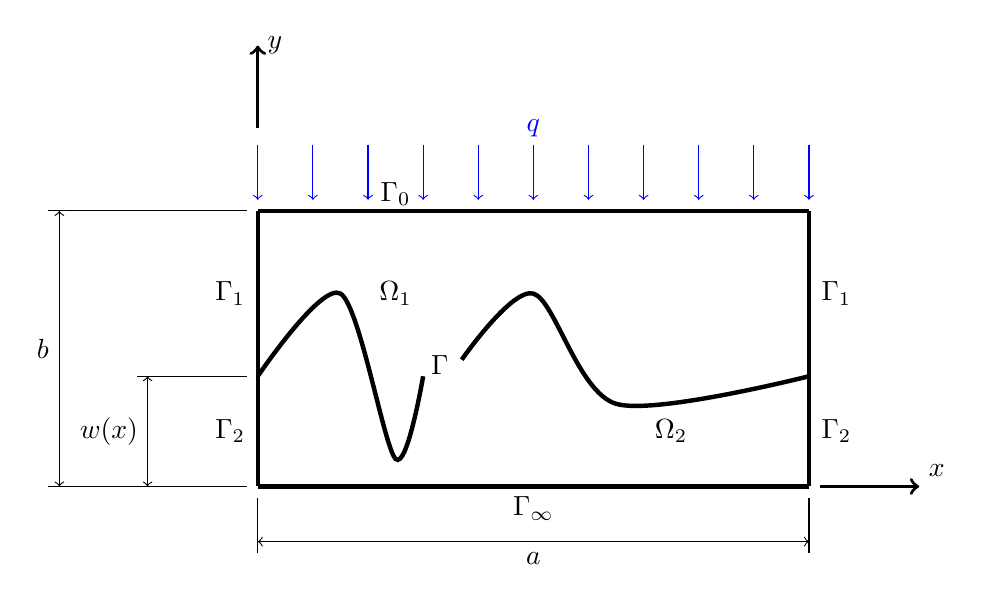
\begin{tikzpicture}[scale=0.7]

	\draw [ultra thick] (0, 0) -- (10, 0);
	%\draw [ultra thick] (0, 2) -- (7, 2);
	%\draw [ultra thick] (8, 2) -- (10, 2);
	\draw [ultra thick] plot [smooth] coordinates {(0, 2) (1.5, 3.5) (2.5, 0.5) (3, 2)};
	\draw [ultra thick] plot [smooth] coordinates {(3.7, 2.3) (5, 3.5) (6.5, 1.5) (10, 2)};
	\draw [ultra thick] (0, 5) -- (10, 5);
	\draw [ultra thick] (0, 0) -- (0, 5);
	\draw [ultra thick] (10, 0) -- (10, 5);
	
	\draw (2.5, 3.5) node {$\Omega_1$};
	\draw (7.5, 1) node {$\Omega_2$};	
	\draw (3.3, 2.2) node {$\Gamma$};
	\draw (-0.5, 3.5) node {$\Gamma_1$};
	\draw (-0.5, 1) node {$\Gamma_2$};
	\draw (10.5, 3.5) node {$\Gamma_1$};
	\draw (10.5, 1) node {$\Gamma_2$};
	\draw (5, -0.4) node {$\Gamma_\infty$};
	\draw (2.5, 5.3) node {$\Gamma_0$};
	\draw [blue](5, 6.5) node {$q$};
	\draw (5, -1.3) node {$a$};
	\draw (-3.9, 2.5) node {$b$};
	\draw (-2.7, 1) node {$w(x)$};
	
	\node [above right] at (12, 0) {$x$};
	\node [right] at (0, 8) {$y$};
	
	\draw [->, blue] (0, 6.2) -- (0, 5.2);
	\draw [->, blue] (1, 6.2) -- (1, 5.2);
	\draw [->, blue] (2, 6.2) -- (2, 5.2);
	\draw [->, blue] (3, 6.2) -- (3, 5.2);
	\draw [->, blue] (4, 6.2) -- (4, 5.2);
	\draw [->, blue] (5, 6.2) -- (5, 5.2);
	\draw [->, blue] (6, 6.2) -- (6, 5.2);
	\draw [->, blue] (7, 6.2) -- (7, 5.2);
	\draw [->, blue] (8, 6.2) -- (8, 5.2);
	\draw [->, blue] (9, 6.2) -- (9, 5.2);
	\draw [->, blue] (10, 6.2) -- (10, 5.2);
	
	\draw [->, very thick] (10.2,0) -- (12,0);
	\draw [->, very thick] (0, 6.5) -- (0,8);
	
	\draw [-] (0, -0.2) -- (0, -1.2);
	\draw [-] (10, -0.2) -- (10, -1.2);
	\draw [<->] (0, -1) -- (10, -1);
	
	\draw [-] (-0.2, 0) -- (-3.8, 0);
	\draw [-] (-0.2, 5) -- (-3.8, 5);
	\draw [-] (-0.2, 2) -- (-2.2, 2);
	\draw [<->] (-3.6, 0) -- (-3.6, 5);
	\draw [<->] (-2.0, 0) -- (-2.0, 2);

\end{tikzpicture}
\caption{Geometria do problema físico}
\label{fig2}
\end{center}
\end{figure}

Considera-se então um corpo de prova ($\Omega$) de seção transversal retangular composto por dois materiais ou regiões isotrópicas ($\Omega_1$ e $\Omega_2$), com
condutividades térmicas correspondentes $k_1$  e $k_2$, colocados em contato,
criando uma interface $\Gamma$ na qual se assume a existência de uma CTC variável com a posição $h_c(x)$.
As superfícies laterais ($\Gamma_1$ e $\Gamma_2$) das duas camadas são mantidas isoladas termicamente;
a superfície inferior ($\Gamma_\infty$) é submetida a uma temperatura prescrita; a superfície superior ($\Gamma_0$) é submetida
a um fluxo de calor por unidade de área $q$. A interseção de qualquer plano paralelo ao plano coordenado $xy$ com a interface $\Gamma$ gera uma
curva descrita por uma equação da forma $y = w(x)$.

Resumidamente, as seguintes hipóteses simplificadores foram adotadas:
\begin{itemize}
  \item O problema de condução de calor sobre o corpo de prova é em regime estacionário: $\displaystyle\frac{\partial T}{\partial t} = 0$;
  \item As condutividades térmicas $k_1$ e $k_2$ dos materiais são constantes;
  \item A variação espacial da CTC é unidimensional: $h_c \equiv h_c(x)$;
  \item O fluxo de calor $q$ sobre a superfície superior $\Gamma_0$ é constante e uniformemente distribuído;
  \item Não há dependência dos campos de temperatura com a componente $z$, ou seja, $T \equiv T(x, y)$; e
  \item Condição de contorno de terceiro tipo, ou de Robin, na interface $\Gamma$:
  		\begin{equation*}
  			-k_1\frac{\partial T_1}{\partial \mathbf{n}_1} = h_c(T_1 - T_2),
  		\end{equation*}   
\end{itemize} 
onde
$\mathbf{n}_1$ é o vetor normal à superfície $\Gamma$ e apontando para fora da região $\Omega_1$, e $T_1$ e $T_2$ são as temperaturas
correspondentes respectivamente às camadas $\Omega_1$ e $\Omega_2$, verificadas na interface $\Gamma$.

\subsection{Formulação matemática do problema direto}\label{sec_formulacao_direta}
Com base nas observações anteriores, podemos formular o problema direto de condução de calor em regime permanente através do corpo de prova $\Omega$ como segue: 

\begin{subequations}
\begin{alignat}{2}
	& \nabla^2 T_1 = 0 \quad\quad\quad\quad\quad && \text{ em } \Omega_1 \label{harm_T1} \\ \nonumber \\
	& -k_1 \frac{\partial T_1}{\partial\mathbf{n}_1} = q && \text{ em } \Gamma_0  \label{cc_T1_2} \\ \nonumber \\
	& \frac{\partial T_1}{\partial \mathbf{n}_1} = 0 && \text{ em }  \Gamma_1 \label{cc_T1_1} \\ \nonumber \\
	& -k_1 \frac{\partial T_1}{\partial\mathbf{n}_1} = h_c(T_1-T_2) \quad\quad\quad\quad\quad\quad\quad\quad && \text{ em }  \Gamma \label{cc_grad_T1} \\ \nonumber \\
	& \nabla^2 T_2 = 0 && \text{ em }  \Omega_2 \label{harm_T2} \\ \nonumber \\
	& \frac{\partial T_2}{\partial \mathbf{n}_2} = 0 && \text{ em }  \Gamma_2 \label{cc_T1_3} \\ \nonumber \\
	& T_2 = 0 && \text{ em }  \Gamma_\infty \label{cc_T1_4} \\ \nonumber \\
	& k_2\frac{\partial T_2}{\partial\mathbf{n}_2} = - k_1\frac{\partial T_1}{\partial\mathbf{n}_1} && \text{ em }  \Gamma \label{cc_T1_5}
\end{alignat}
\end{subequations}

A atribuição do valor zero à temperatura na superfície inferior $\Gamma_\infty$ do corpo $\Omega_2$, ao invés do valor prescrito, é uma simplificação
que permite a homogeneização da condição de contorno \eqref{cc_T1_4}. De fato, representando o valor da temperatura prescrita nessa superfície como $T^\star$,
o campo de temperaturas na região $\Omega_2$ seria dado por
\begin{equation}
	T_2^\star = T_2 + T^\star
\end{equation}


\section{Problema inverso}\label{sec_prob_inv}

O problema inverso proposto neste trabalho é a estimativa da condutância térmica de contato $h_c$ na interface $\Gamma$ entre os corpos materiais
postos em contato $\Omega_1$ e $\Omega_2$, segundo o arranjo físico ilustrado na figura \ref{fig2}, conforme estabelecido na equação \eqref{eq:definicao_1}:
\begin{equation}
	h_c = \frac{q_c}{\Delta T_c}
\end{equation}

O fluxo de calor por unidade de área $q_c$ e o salto de temperatura $\Delta T_c$, ambos tomados na interface de contato, serão estimados de forma
indireta e não intrusiva, através do emprego do conceito de funcional de reciprocidade (FR), que será explicado na próxima seção.

A estimativa da CTC será feita através de medidas de temperaturas tomadas na superfície superior $\Gamma_0$ do corpo de prova, submetida a um fluxo
de calor por unidade de área $q$. As superfícies laterais $\Gamma_1$ e $\Gamma_2$ são mantidas termicamente isoladas, e a temperatura da superfície
inferior $\Gamma_\infty$ é mantida constante. As características termofísicas dos corpos materiais em contato são conhecidas, a saber, as 
condutividades térmicas $k_1$ e $k_2$, bem como as dimensões $a$ e $b$ do corpo de prova e a curva $y = w(x)$, que descreve geometricamente a interface
de contato entre os corpos. 

\subsection{Definição do conceito de funcional de reciprocidade}

A ideia do funcional de reciprocidade teve origem a partir do trabalho de \cite{artigo_andrieux}, que introduziram o conceito de funcional de descontinuidade
de reciprocidade (do inglês, \textit{reciprocity gap functional}). Segundo os autores, a intenção era levantar informações sobre a estrutura interna de
um corpo a partir de grandezas medidas na fronteira deste corpo, posto que tais grandezas estivessem relacionadas a um fenômeno físico descrito por
equações diferenciais parciais elípticas. As informações obtidas, por sua vez, seriam caracterizações de descontinuidades, espaços vazios internos ou inclusões
de materiais, entendidas de forma geral como ``perturbações''. Os autores, no referido trabalho, concentraram-se no problema específico de identificação
de falhas planas no interior de corpos materiais.

Nesse sentido, a introdução de uma perturbação a um corpo material geraria uma resposta à aplicação de um campo escalar diferente da obtida se
essa perturbação não estivesse presente. Seja então um fluxo de uma grandeza escalar $\Phi_m$ imposto à fronteira externa $\partial\Omega$ de um corpo material
$\Omega$, e seja $U_m$ a medida de um campo escalar $u$ em equilíbrio, tomada na mesma fronteira (figura \ref{fig3}). Exemplos de grandezas dessa natureza são
temperatura e fluxo de calor, ou deformação e vetor tensão. 
\begin{figure}[h!b]
\begin{center}
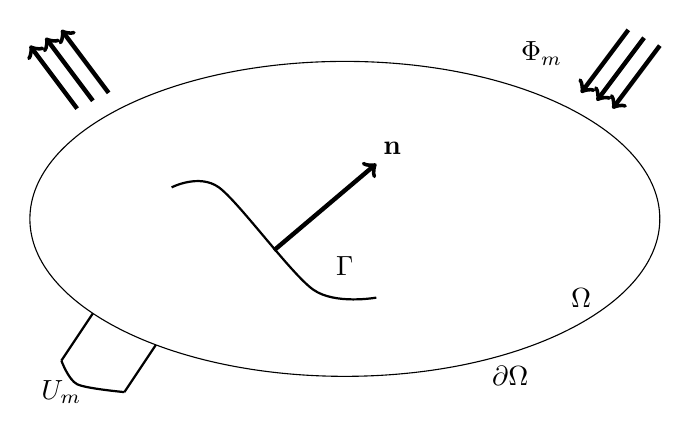
\begin{tikzpicture}[scale=1.0]
	\draw (0,0) ellipse (4cm and 2cm);
	\draw [->, ultra thick] (-3.4cm, 1.4cm) -- (-4.0cm, 2.2cm);
	\draw [->, ultra thick] (-3.2cm, 1.5cm) -- (-3.8cm, 2.3cm);
	\draw [->, ultra thick] (-3.0cm, 1.6cm) -- (-3.6cm, 2.4cm);
	\draw [->, ultra thick] (4.0cm, 2.2cm) -- (3.4cm, 1.4cm);
	\draw [->, ultra thick] (3.8cm, 2.3cm) -- (3.2cm, 1.5cm);
	\draw [->, ultra thick] (3.6cm, 2.4cm) -- (3.0cm, 1.6cm);
	\draw (2.5, 2.1) node {$\Phi_m$};
	\draw [thick] plot [smooth] coordinates {(-2.2, 0.4) (-1.6, 0.4) (-0.4, -0.9) (0.4, -1.0)};
	\draw (0.0, -0.6) node {$\Gamma$};
	\draw [->, ultra thick] (-0.9, -0.4) -- (0.4, 0.7);
	\draw (0.6, 0.9) node {$\mathbf{n}$};
	\draw (3.0, -1.0) node {$\Omega$};
	\draw (2.1, -2.0) node {$\partial\Omega$};
	\draw [thick] (-3.2cm, -1.2cm) -- (-3.6cm, -1.8cm);
	\draw [thick] (-2.4cm, -1.6cm) -- (-2.8cm, -2.2cm);
	\draw [thick] plot [smooth] coordinates {(-3.6cm, -1.8cm) (-3.4, -2.1) (-2.8cm, -2.2cm)};
	\draw (-3.6cm, -2.2cm) node {$U_m$};
\end{tikzpicture}
\caption{Corpo material $\Omega$ (adaptado de \citeauthor{artigo_andrieux}, \citeyear{artigo_andrieux})}
\label{fig3}
\end{center}
\end{figure}

A expressão que define o funcional de descontinuidade de reciprocidade, estabelecida por Andrieux e Ben Abda, é dada por:
\begin{align}
	RG(v) = \int_{\partial\Omega} \left( \Phi_m v - U_m \nabla v \cdot \mathbf{n} \right) \label{definicao_rgap}
\end{align}
onde $v$ é um outro campo potencial em equilíbrio em $\Omega$.

Os autores afirmam que quando não há descontinuidades no interior de $\Omega$, a integral \eqref{definicao_rgap} se anula. Desse modo, o funcional de descontinuidade de reciprocidade
forneceria uma medida do desvio provocado num campo escalar $u$ no corpo $\Omega$ submetido a um fluxo $\Phi_m$ em sua superfície, se esse corpo
possuir uma descontinuidade $\Gamma$ em seu interior.

É importante destacar que a integral \eqref{definicao_rgap} é calculada sobre o contorno da fronteira do corpo material $\Omega$, onde as grandezas envolvidas devem
ser efetivamente conhecidas. Assim, é possível inferir características no interior do corpo a partir de medições tomadas em seu contorno.

\subsection{Aplicação do funcional de reciprocidade na dedução da expressão da estimativa da condutância térmica de contato}\label{secao_sobre_fr}

Baseados no conceito de funcional de descontinuidade de reciprocidade, \cite{reciproc_2} apresentaram um trabalho pioneiro em que estabeleceram uma
técnica não intrusiva e não iterativa para solução de problemas inversos de transferência de calor, voltada para a estimativa da resistência térmica de
contato (RTC) entre dois corpos. A metodologia aplicada nesta dissertação, baseada no referido trabalho e em trabalhos posteriores em que aquele conceito
foi utilizado \citep{artigo_padilha_3}, será descrita nos parágrafos a seguir. 

\cite{reciproc_2} adaptaram o termo original definido em \eqref{definicao_rgap} para o problema formulado na seção \ref{sec_formulacao_direta},
introduzindo o conceito de funcional de reciprocidade (FR) através da seguinte expressão:
\begin{align}
	\Re(F) = \int_{\Gamma_0}\left[\left(\frac{-q}{k_1}\right)F - Y\frac{\partial F}{\partial\mathbf{n_1}}\right]d\Gamma_0
	\label{def_funcional_reciprocidade}
\end{align}
onde $F$ é uma função associada a um campo potencial auxiliar em equilíbrio em $\Omega_1$, $k_1$ é a condutividade térmica do material $\Omega_1$, $q$ é o fluxo de calor por unidade de área
aplicado na superfície externa $\Gamma_0$ e $Y$ são medidas de temperatura tomadas na mesma superfície $\Gamma_0$. O vetor $\mathbf{n_1}$ é o vetor normal à superfície
$\Gamma_0$ e apontando para fora do contorno do material $\Omega_1$.

De forma análoga à equação \eqref{definicao_rgap}, a equação \eqref{def_funcional_reciprocidade} permite medir a alteração do campo de temperatura
gerado por um fluxo de calor por unidade de área $q$ aplicado na superfície externa $\Gamma_0$ do material compósito $\Omega$ devido à existência
de uma descontinuidade $\Gamma$ em seu interior; essa alteração está relacionada à existência de uma RTC nessa interface. No caso de não haver descontinuidade
em $\Omega$, a integral \eqref{def_funcional_reciprocidade} se anula.

Em seu trabalho, \cite{reciproc_2} formulam dois problemas difusivos para determinação de duas classes de funções auxiliares $F_1$ e $G_1$, no mesmo domínio físico da região compreendida
por $\Omega_1$. Os problemas formulados são análogos ao problema de difusão de temperatura formulado em \eqref{harm_T1}--\eqref{cc_T1_5}, porém empregando condições de contorno apropriadas, que
serão detalhadas na seção \ref{secao_probs_aux}.

Através dessas condições de contorno, os autores demonstram as seguintes identidades:
\begin{align}
	k_1 \int_{\Gamma_0}\left[\left(\frac{-q}{k_1}\right)F_1 - Y\frac{\partial F_1}{\partial\mathbf{n_1}}\right]d\Gamma_0
	=
	\int_\Gamma k_1 \frac{\partial F_1}{\partial\mathbf{n_1}}\left(T_1 - T_2\right)d\Gamma
	\label{identidade_T}
\end{align}
\begin{align}
	k_1 \int_{\Gamma_0}\left[\left(\frac{-q}{k_1}\right)G_1 - Y\frac{\partial G_1}{\partial\mathbf{n_1}}\right]d\Gamma_0
	=
	\int_\Gamma -k_1 G_1 \frac{\partial T_1}{\partial\mathbf{n_1}}d\Gamma
	\label{identidade_q}
\end{align}

Os termos à esquerda das equações \eqref{identidade_T} e \eqref{identidade_q} são, a menos da constante multiplicativa $k_1$, a definição do funcional de reciprocidade para as 
funções auxiliares $F_1$ e $G_1$.

As integrais à direita têm um significado importante. É possível observar que elas são calculadas \textit{ao longo da interface de contato} $\Gamma$. O termo
$T_1 - T_2$ é exatamente \textit{o salto de temperatura através da interface} $\Gamma$, enquanto que o termo $\displaystyle-k_1 \frac{\partial T_1}{\partial\mathbf{n_1}}$
é exatamente \textit{o fluxo de calor por unidade de área através da interface} $\Gamma$ (cf. equação \eqref{eq:definicao_2}). Desse modo, as identidades \eqref{identidade_T} e \eqref{identidade_q}
relacionam \textit{as medidas
do salto de temperatura e de fluxo de calor na interface} $\Gamma$ -- grandezas cuja razão fornece a RTC sobre a interface -- com \textit{as medidas de temperatura} $Y$ \textit{tomadas na superfície} $\Gamma_0$.

Estas mesmas integrais também podem ser interpretadas à luz dos conceitos de Álgebra Linear \citep{livro_axler}. Sob esse ponto de vista, os termos
$\displaystyle k_1 \frac{\partial F}{\partial\mathbf{n_1}}$, $T_1 - T_2$, $G$ e $\displaystyle-k_1 \frac{\partial T_1}{\partial\mathbf{n_1}}$ podem ser identificados como funções pertencentes a um espaço
linear de funções, denotado por $L^2(\Gamma)$, em que se define a operação de produto interno como segue:
\begin{align}
	\langle f_1, f_2\rangle_{L^2(\Gamma)} = \int_\Gamma f_1(\Gamma) f_2(\Gamma) d\Gamma \label{definicao_innner_product}
\end{align} 
onde $f_1$ e $f_2$ são funções reais, contínuas por partes, definidas a longo do contorno $\Gamma$ sobre o qual é calculada a integral. A norma de uma
função, que é uma métrica análoga ao ``comprimento'' ou ``distância'', é definida nesse espaço linear como\footnote{A partir desse ponto, o subscrito ${L^2(\Gamma)}$ será
subentendido nas transcrições de produtos internos, para fins de simplificação gráfica das equações.}:
\begin{align}
	\norm{f} = \sqrt{\langle f, f\rangle}
\end{align}

A partir de parametrizações convenientes dos problemas difusivos auxiliares, é possível levantar duas famílias de funções auxiliares $F_{1,j}, j=1,2,\ldots N_1$
e $G_{1,j}, j=1,2,\ldots N_2$. Assim, através da definição de produto interno em \eqref{definicao_innner_product} e da definição de funcional de reciprocidade em \eqref{def_funcional_reciprocidade},
as identidades \eqref{identidade_T} e \eqref{identidade_q} podem ser reescritas como:
\begin{align}
	k_1 \Re(F_{1,j})
	=
	\left\langle \left[T_1 - T_2\right]_\Gamma, \beta_j\right\rangle
	\label{identidade_T_inner}
\end{align}
\begin{align}
	k_1 \Re(G_{1,j})
	=
	\left\langle  -k_1 \frac{\partial T_1}{\partial\mathbf{n_1}}\bigg|_\Gamma, \gamma_j\right\rangle
	\label{identidade_q_inner}
\end{align}
onde
\begin{align}
	\beta_j = k_1 \frac{\partial F_{1,j}}{\partial\mathbf{n_1}}\bigg|_\Gamma \label{expressao_define_beta}
\end{align}
\begin{align}
	\gamma_j = G_{1,j}\big|_\Gamma \label{expressao_define_gamma}
\end{align}

Com base no trabalho de \cite{artigo_padilha_3}, será proposta uma escolha de parametrização de condições de contorno dos problemas auxiliares de modo que as funções
$\beta_j, j=1,2,\ldots N_1$ e $\gamma_j, j=1,2,\ldots N_2$ formem dois conjuntos ortonormais, isto é:
\begin{align}
	\left\langle  \beta_m, \beta_n \right\rangle = \left\lbrace
		\begin{matrix}
		0, & m \neq n \\
		1, & m = n 
		\end{matrix}
	\right.
\end{align}
\begin{align}
	\left\langle  \gamma_m, \gamma_n \right\rangle = \left\lbrace
		\begin{matrix}
		0, & m \neq n \\
		1, & m = n 
		\end{matrix}
	\right.
\end{align}

Nessas condições, cada um dos conjuntos define um subespaço linear contido no espaço linear $L^2(\Gamma)$. Os subespaços lineares gerados pela bases
ortonormais $\beta_j$ e $\gamma_j$ serão denotados respectivamente por $L^2(\Gamma, \beta)$ e $L^2(\Gamma, \gamma)$.

Por definição, a \textit{projeção ortogonal} de uma função $f$ pertencente ao espaço linear $L^2(\Gamma)$ sobre o subespaço linear $L^2(\Gamma, \epsilon)$
gerado por uma base ortonormal $\epsilon_j, j=1,2,\ldots,N$ é dada por:
\begin{align}
	P_{L^2(\Gamma, \epsilon)}[f] = \sum_{j=1}^N \left\langle f, \epsilon_j \right\rangle \epsilon_j
\end{align}

A projeção ortogonal provê uma forma aproximada de se representar uma função $f$ como combinação linear dos elementos de uma base ortonormal de
funções. Com efeito, seja $g$ uma função em $L^2(\Gamma, \epsilon)$, e que portanto pode ser expandida como uma combinação linear dos elementos da base $\epsilon_j$. Uma métrica de
avaliação da ``distância'' entre as funções $f$ e $g$ é dada pela norma da diferença entre essas funções. O menor valor possível para essa norma ocorre
quando a função $g$ for a projeção ortogonal de $f$ sobre $L^2(\Gamma, \epsilon)$ \citep{livro_axler}. Ou seja,
\begin{align}
	\norm{f - P_{L^2(\Gamma, \epsilon)}[f]} \le \norm{f - g}, \forall g \in L^2(\Gamma, \epsilon)
\end{align}

Dessa forma, o salto de temperatura e o fluxo de calor por unidade de área na interface $\Gamma$ podem ser representados de forma aproximada através de projeções
ortogonais sobre os subespaços lineares $L^2(\Gamma, \beta)$ e $L^2(\Gamma, \gamma)$ respectivamente:
\begin{align}
[T_1 - T_2]_\Gamma \approx \sum_{j=1}^{N_1} \left\langle  \left[T_1 - T_2\right]_\Gamma, \beta_j \right\rangle \beta_j
\end{align}
\begin{align}
	- k_1 \frac{\partial T_1}{\partial\mathbf{n_1}}\bigg|_\Gamma \approx \sum_{j=1}^{N_2} \left\langle  -k_1 \frac{\partial T_1}{\partial\mathbf{n_1}}\bigg|_\Gamma, \gamma_j \right\rangle \gamma_j
\end{align}

Aplicando as identidades \eqref{identidade_T_inner} e \eqref{identidade_q_inner} às equações acima, e assumindo que as projeções ortogonais representam
de forma razoável as funções correspondentes, pode-se escrever:
\begin{align}
	[T_1 - T_2]_\Gamma = \sum_{j=1}^{N_1} k_1 \Re(F_{1,j}) \beta_j \label{resultado_1}
\end{align}
\begin{align}
	- k_1 \frac{\partial T_1}{\partial\mathbf{n_1}}\bigg|_\Gamma = \sum_{j=1}^{N_2} k_1 \Re(G_{1,j}) \gamma_j \label{resultado_2}
\end{align}

Finalmente, substituindo os resultados obtidos em \eqref{resultado_1} e \eqref{resultado_2} na definição de condutância térmica de contato,
\eqref{eq:definicao_3}, obtemos a seguinte relação:
\begin{align}
	& h_c % = \frac{- k_1 \displaystyle\frac{\partial T_1}{\partial\mathbf{n_1}}\bigg|_\Gamma}{[T_1 - T_2]_\Gamma} 
	= \frac{\displaystyle\sum_{j=1}^{N_2} \Re(G_{1,j}) \gamma_j}{\displaystyle\sum_{j=1}^{N_1} \Re(F_{1,j}) \beta_j}
	\label{equacao_definicao_f_r}
\end{align}
ou, de forma mais explícita:
\begin{align}
	& h_c % = \frac{- k_1 \displaystyle\frac{\partial T_1}{\partial\mathbf{n_1}}\bigg|_\Gamma}{[T_1 - T_2]_\Gamma} 
	= \frac{\displaystyle\sum_{j=1}^{N_2} \gamma_j\int_{\Gamma_0}\left[\left(\frac{-q}{k_1}\right)G_{1,j} - Y\frac{\partial G_{1,j}}{\partial\mathbf{n_1}}\right]d\Gamma_0}{\displaystyle\sum_{j=1}^{N_1} \beta_j \int_{\Gamma_0}\left[\left(\frac{-q}{k_1}\right)F_{1,j} - Y\frac{\partial F_{1,j}}{\partial\mathbf{n_1}}\right]d\Gamma_0}
	\label{equacao_definicao_f_r_expl}
\end{align}

A expressão \eqref{equacao_definicao_f_r} permite calcular a estimativa da distribuição da CTC ao longo da interface de contato $\Gamma$, conhecendo-se
a distribuição de temperaturas $Y$ medidas na face externa superior do arranjo físico da figura \ref{fig2}, eliminando assim a necessidade prévia de
se conhecer informações e características internas do corpo de prova, tais como rugosidade entre as superfícies em contato, pressão de contato, ou
o fluido presente no interstício. As determinações do salto de temperatura e fluxo de calor por unidade de área na interface de contato são feitas de forma indireta, através
das expansões em funções ortonormais expressas em \eqref{resultado_1} e \eqref{resultado_2}, o que indica o caráter não intrusivo da técnica.

Quanto ao aspecto numérico-computacional, é possível notar que as integrais que fornecem os funcionais de reciprocidade só precisam ser calculadas
uma única vez, para uma determinada caracterização geométrica e termofísica do problema. As classes de funções $F_{1,j}$ e $G_{1,j}$, obtidas através da resolução dos
problemas difusivos auxiliares, dependem unicamente das
características geométricas (comprimento e largura do corpo de prova, e a curva $y = w(x)$ que descreve o formato da interface)
e termofísicas (condutâncias térmicas $k_1$ e $k_2$ dos materiais em contato). Por essa razão, o método é classificado como não iterativo, visto que
a obtenção da estimativa da CTC em algum ponto sobre a interface se resume à substituição dos valores de $\beta_j$ e $\gamma_j$ avaliados naquele
ponto nos somatórios da equação \eqref{equacao_definicao_f_r}.

Por último, é importante destacar que a expressão \eqref{equacao_definicao_f_r} permite a estimativa da CTC para qualquer formato de interface $\Gamma$,
desde que se conheça a sua descrição analítica representada pela curva $y = w(x)$. O caso particular em que a interface é plana e paralela às bases do corpo
de prova foi resolvido analiticamente por \cite{tese_padilha}.

% \subsection{Comentários sobre o caso particular de interface de contato plana}
% 
% O problema inverso definido pelo arranjo físico representado na figura \ref{fig2}, juntamente com as equações \eqref{harm_T1} -- \eqref{cc_T1_5}, é uma
% generalização de um problema mais simples em que a interface de contato é um plano paralelo às faces inferior e superior do corpo de prova, conforme
% ilustrado na \ref{fig4}.
\begin{figure}[h!b]
\begin{center}
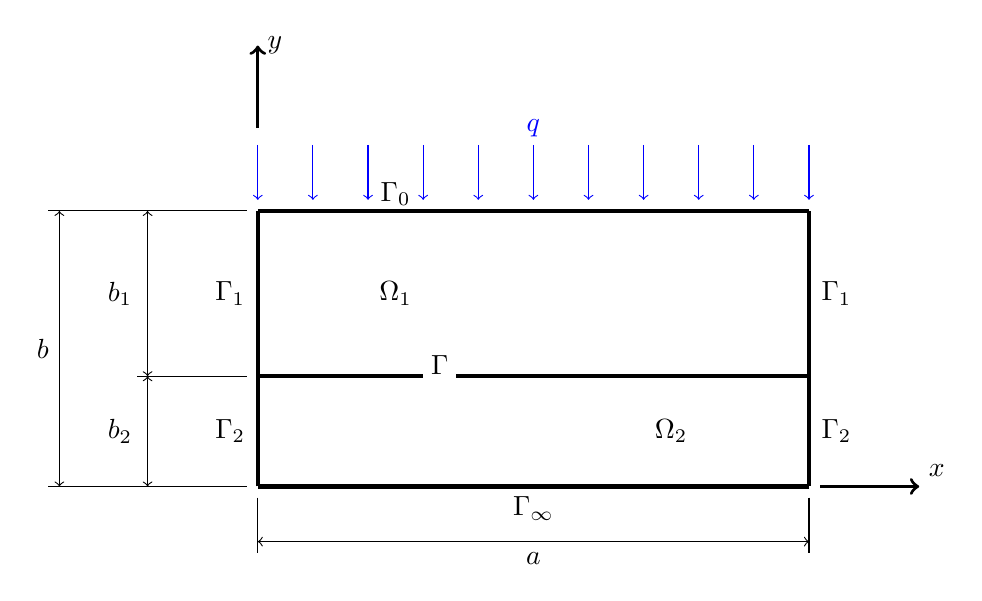
\begin{tikzpicture}[scale=0.7]

	\draw [ultra thick] (0, 0) -- (10, 0);
	%\draw [ultra thick] (0, 2) -- (7, 2);
	%\draw [ultra thick] (8, 2) -- (10, 2);
	\draw [ultra thick] (0, 5) -- (10, 5);
	\draw [ultra thick] (0, 2.0) -- (3.0, 2.0);
	\draw [ultra thick] (3.6, 2.0) -- (10, 2.0);
	\draw [ultra thick] (0, 0) -- (0, 5);
	\draw [ultra thick] (10, 0) -- (10, 5);

	\draw (2.5, 3.5) node {$\Omega_1$};
	\draw (7.5, 1) node {$\Omega_2$};
	\draw (3.3, 2.2) node {$\Gamma$};
	\draw (-0.5, 3.5) node {$\Gamma_1$};
	\draw (-0.5, 1) node {$\Gamma_2$};
	\draw (10.5, 3.5) node {$\Gamma_1$};
	\draw (10.5, 1) node {$\Gamma_2$};
	\draw (5, -0.4) node {$\Gamma_\infty$};
	\draw (2.5, 5.3) node {$\Gamma_0$};
	\draw [blue](5, 6.5) node {$q$};
	\draw (5, -1.3) node {$a$};
	\draw (-3.9, 2.5) node {$b$};
	\draw (-2.5, 1) node {$b_2$};
	\draw (-2.5, 3.5) node {$b_1$};

	\node [above right] at (12, 0) {$x$};
	\node [right] at (0, 8) {$y$};

	\draw [->, blue] (0, 6.2) -- (0, 5.2);
	\draw [->, blue] (1, 6.2) -- (1, 5.2);
	\draw [->, blue] (2, 6.2) -- (2, 5.2);
	\draw [->, blue] (3, 6.2) -- (3, 5.2);
	\draw [->, blue] (4, 6.2) -- (4, 5.2);
	\draw [->, blue] (5, 6.2) -- (5, 5.2);
	\draw [->, blue] (6, 6.2) -- (6, 5.2);
	\draw [->, blue] (7, 6.2) -- (7, 5.2);
	\draw [->, blue] (8, 6.2) -- (8, 5.2);
	\draw [->, blue] (9, 6.2) -- (9, 5.2);
	\draw [->, blue] (10, 6.2) -- (10, 5.2);

	\draw [->, very thick] (10.2,0) -- (12,0);
	\draw [->, very thick] (0, 6.5) -- (0,8);

	\draw [-] (0, -0.2) -- (0, -1.2);
	\draw [-] (10, -0.2) -- (10, -1.2);
	\draw [<->] (0, -1) -- (10, -1);

	\draw [-] (-0.2, 0) -- (-3.8, 0);
	\draw [-] (-0.2, 5) -- (-3.8, 5);
	\draw [-] (-0.2, 2) -- (-2.2, 2);
	\draw [<->] (-3.6, 0) -- (-3.6, 5);
	\draw [<->] (-2.0, 0) -- (-2.0, 2);
	\draw [<->] (-2.0, 2) -- (-2.0, 5);

\end{tikzpicture}
\caption{Geometria do problema físico resolvido por \cite{reciproc_2}}
\label{fig4}
\end{center}
\end{figure}
% 
% Na resolução deste problema inverso, \cite{reciproc_2} deduziram uma versão mais simples da expressão \eqref{equacao_definicao_f_r}:
% \begin{align}
% 	& h_c % = \frac{- k_1 \displaystyle\frac{\partial T_1}{\partial\mathbf{n_1}}\bigg|_\Gamma}{[T_1 - T_2]_\Gamma} 
% 	= \frac{\displaystyle\sum_{j=1}^N \Re(G_{1,j}) \phi_j}{\displaystyle\sum_{j=1}^N \Re(F_{1,j}) \phi_j}
% 	\label{equacao_definicao_f_r_simples}
% \end{align}
% 
% As funções $\phi_j, j=1,2\ldots,N$ foram definidas através de funções seno e cosseno, ortogonais
% no intervalo $0 \le x \le a$.
% 
% Uma vez que, para esse problema, $\phi_j = \beta_j = \gamma_j$, foram definidas as seguintes condições de contorno para as famílias de 
% funções $F_{1,j}$ e $G_{1,j}$: 
% 
% 
%  
% . Os problemas difusivos auxiliares que fornecem as funções $F_j$ e $G_j$
% foram resolvidos através do Método das Soluções Fundamentais 

\section{Formulação dos problemas auxiliares e solução via Transformação Integral Clássica}\label{secao_probs_aux}

Será apresentada agora a formulação matemática dos problemas auxiliares cujas soluções fornecem as classes de funções auxiliares $F_1$ e $G_1$, necessárias
para obtenção da estimativa do perfil de CTC através da equação \eqref{equacao_definicao_f_r}. As soluções desses problemas serão desenvolvidas analiticamente através do
emprego da Técnica da Transformada Integral Clássica (CITT). 

Os problemas auxiliares são definidos com base nos problemas apresentados no artigo de \cite{reciproc_2} e modificados por \cite{tese_abreu}.  

\subsection{Primeiro problema auxiliar}\label{secao_do_primeiro}

Sejam duas famílias de funções harmônicas $F_{1, j}$ e $F_{2, j}$, definidas respectivamente nos domínios $\Omega_1$ e $\Omega_2$.Define-se assim o primeiro
problema auxiliar, relacionado ao salto de temperatura na interface $\Gamma$ através das seguintes equações:

\begin{subequations}
	\begin{alignat}{2}
	& \nabla^2 F_{1,j} = 0 \quad\quad\quad\quad\quad && \text{ em } \Omega_1 \label{funcao_F_harm_T1} \\ \nonumber \\
	& F_{1,j} = \psi_j && \text{ em } \Gamma_0  \label{funcao_F_cc_T1_2} \\ \nonumber \\
	& \frac{\partial F_{1,j}}{\partial \mathbf{n}_1} = 0 && \text{ em }  \Gamma_1 \label{funcao_F_cc_T1_1} \\ \nonumber \\
	& F_{1,j} = F_{2, j} \quad\quad\quad\quad\quad\quad\quad\quad && \text{ em }  \Gamma \label{funcao_F_cc_grad_T1} \\ \nonumber \\
	& \nabla^2 F_{2,j} = 0 && \text{ em }  \Omega_2 \label{funcao_F_harm_T2} \\ \nonumber \\
	& \frac{\partial F_{2,j}}{\partial \mathbf{n}_2} = 0 && \text{ em }  \Gamma_2 \label{funcao_F_cc_T1_3} \\ \nonumber \\
	& F_{2,j} = 0 && \text{ em }  \Gamma_\infty \label{funcao_F_cc_T1_4} \\ \nonumber \\
	& k_2\frac{\partial F_{2, j}}{\partial\mathbf{n}_2} = - k_1\frac{\partial F_{1,j}}{\partial\mathbf{n}_1} = -\beta_j && \text{ em }  \Gamma \label{funcao_F_cc_T1_5}
	\end{alignat}
\end{subequations}

Nas equações acima, para compor a condição de contorno na interface superior $\Gamma_0$, foi introduzida uma família de funções $\psi_j(x), j=1,2,\ldots N_1$, a serem definidas posteriormente. A solução do sistema de equações \eqref{funcao_F_harm_T1} a \eqref{funcao_F_cc_T1_5} será escrita em termos daquelas funções. 

\subsection{Segundo problema auxiliar}\label{secao_do_segundo}
Seja a família de funções harmônicas $G_{1, j}$, definida no domínio $\Omega_1$. Define-se assim o segundo
problema auxiliar, relacionado ao fluxo de calor por unidade de área através da interface, $\Gamma$ através das seguintes equações:
\begin{subequations}
	\begin{alignat}{2}
	& \nabla^2 G_{1,j} = 0 \quad\quad\quad\quad\quad && \text{ em } \Omega_1 \label{funcao_G_harm_T1} \\ \nonumber \\
	& G_{1,j} = \phi_j && \text{ em } \Gamma_0  \label{funcao_G_cc_T1_2} \\ \nonumber \\
	& \frac{\partial G_{1,j}}{\partial \mathbf{n}_1} = 0 && \text{ em }  \Gamma_1 \label{funcao_G_cc_T1_1} \\ \nonumber \\
	& \frac{\partial G_{1,j}}{\partial\mathbf{n}_1} = 0 \quad\quad\quad\quad\quad\quad\quad\quad && \text{ em }  \Gamma \label{funcao_G_cc_grad_T1}
	\end{alignat}
\end{subequations}

Assim como no primeiro problema, a fim de compor a condição de contorno na interface superior $\Gamma_0$, foi introduzida uma família de funções $\phi_j(x), j=1,2,\ldots N_2$, que serão definidas posteriormente. A solução do sistema de equações \eqref{funcao_G_harm_T1} a \eqref{funcao_G_cc_grad_T1} será escrita em termos daquelas funções. 

\subsection{Preparação dos problemas auxiliares para aplicação da Técnica da Transformada Integral Clássica}
Os conjuntos de equações \eqref{funcao_F_harm_T1} a \eqref{funcao_F_cc_T1_5} e \eqref{funcao_G_harm_T1} a \eqref{funcao_G_cc_grad_T1}, numa primeira análise,
não estão restritas a algum sistema de coordenadas em particular. Por outro lado, a seção transversal do corpo de prova tem formato retangular; por isso,
a fim de favorecer o uso da Técnica da Transformada Integral Clássica, a ser descrita na próxima seção,
será feita a formulação do problemas auxiliares em termos de coordenadas cartesianas e a redefinição do domínio físico sobre o qual esses problemas
serão resolvidos.

\subsubsection{A Técnica da Transformada Integral Clássica}

A Técnica da Transformada Integral Clássica (do inglês \textit{Classical Integral Transform Technique} - CITT), historicamente baseada no método de separação de variáveis \citep{livro_boyce},
fornece uma abordagem sistemática e eficiente para solução
de problemas difusivos de valor de contorno em regime permanente ou transiente, que envolvam termos não-homogêneos nas equações diferenciais ou nas condições
de contorno \citep{livro_ozisik}. Esta técnica foi recentemente empregada na solução do problema inverso de transferência de calor para determinação da CTC para
uma interface de contato plana, num arranjo semelhante ao da figura \ref{fig4}, fornecendo bons resultados \citep{tese_padilha}. Considerando que o referido problema é um caso particular
de um arranjo mais geral, representado na figura \ref{fig2}, objeto de estudo desta dissertação, foi natural a opção por esta técnica para determinação da solução do problema inverso correspondente.
\begin{figure}[h!b]
\begin{center}
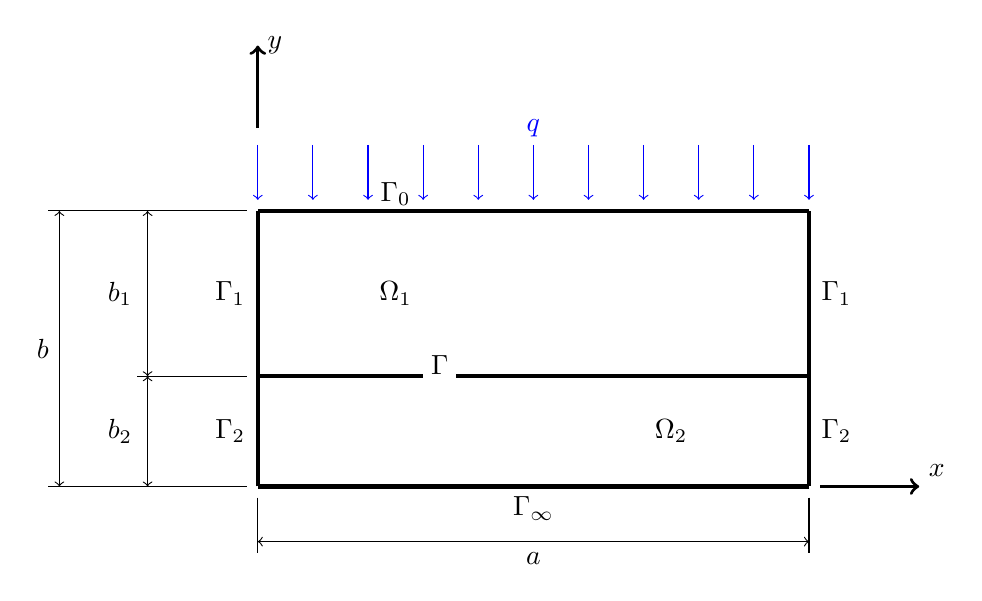
\begin{tikzpicture}[scale=0.7]

	\draw [ultra thick] (0, 0) -- (10, 0);
	%\draw [ultra thick] (0, 2) -- (7, 2);
	%\draw [ultra thick] (8, 2) -- (10, 2);
	\draw [ultra thick] (0, 5) -- (10, 5);
	\draw [ultra thick] (0, 2.0) -- (3.0, 2.0);
	\draw [ultra thick] (3.6, 2.0) -- (10, 2.0);
	\draw [ultra thick] (0, 0) -- (0, 5);
	\draw [ultra thick] (10, 0) -- (10, 5);

	\draw (2.5, 3.5) node {$\Omega_1$};
	\draw (7.5, 1) node {$\Omega_2$};
	\draw (3.3, 2.2) node {$\Gamma$};
	\draw (-0.5, 3.5) node {$\Gamma_1$};
	\draw (-0.5, 1) node {$\Gamma_2$};
	\draw (10.5, 3.5) node {$\Gamma_1$};
	\draw (10.5, 1) node {$\Gamma_2$};
	\draw (5, -0.4) node {$\Gamma_\infty$};
	\draw (2.5, 5.3) node {$\Gamma_0$};
	\draw [blue](5, 6.5) node {$q$};
	\draw (5, -1.3) node {$a$};
	\draw (-3.9, 2.5) node {$b$};
	\draw (-2.5, 1) node {$b_2$};
	\draw (-2.5, 3.5) node {$b_1$};

	\node [above right] at (12, 0) {$x$};
	\node [right] at (0, 8) {$y$};

	\draw [->, blue] (0, 6.2) -- (0, 5.2);
	\draw [->, blue] (1, 6.2) -- (1, 5.2);
	\draw [->, blue] (2, 6.2) -- (2, 5.2);
	\draw [->, blue] (3, 6.2) -- (3, 5.2);
	\draw [->, blue] (4, 6.2) -- (4, 5.2);
	\draw [->, blue] (5, 6.2) -- (5, 5.2);
	\draw [->, blue] (6, 6.2) -- (6, 5.2);
	\draw [->, blue] (7, 6.2) -- (7, 5.2);
	\draw [->, blue] (8, 6.2) -- (8, 5.2);
	\draw [->, blue] (9, 6.2) -- (9, 5.2);
	\draw [->, blue] (10, 6.2) -- (10, 5.2);

	\draw [->, very thick] (10.2,0) -- (12,0);
	\draw [->, very thick] (0, 6.5) -- (0,8);

	\draw [-] (0, -0.2) -- (0, -1.2);
	\draw [-] (10, -0.2) -- (10, -1.2);
	\draw [<->] (0, -1) -- (10, -1);

	\draw [-] (-0.2, 0) -- (-3.8, 0);
	\draw [-] (-0.2, 5) -- (-3.8, 5);
	\draw [-] (-0.2, 2) -- (-2.2, 2);
	\draw [<->] (-3.6, 0) -- (-3.6, 5);
	\draw [<->] (-2.0, 0) -- (-2.0, 2);
	\draw [<->] (-2.0, 2) -- (-2.0, 5);

\end{tikzpicture}
\caption{Geometria do problema físico resolvido por \cite{reciproc_2}}
\label{fig4}
\end{center}
\end{figure}

De acordo com \cite{livro_cotta}, a solução dos problemas via CITT requer a aplicação dos seguintes passos:
\begin{enumerate}[(i)]
	\item Desenvolver o problema de autovalor associado, através da aplicação do método de separação de variáveis à versão homogênea do problema da equação
	diferencial parcial;
	\item Desenvolver o par transformada-inversa apropriado;
	\item Aplicar a transformação integral à equação diferencial parcial do problema de valor de contorno original, empregando as condições de contorno no
	desenvolvimento dos cálculos;
	\item Resolver o sistema de equações diferenciais ordinárias desacopladas gerado a partir da transformação integral; e
	\item Aplicar a fórmula de inversão previamente estabelecida no passo (ii) para construir a solução completa do problema.
\end{enumerate}

Na seção anterior, foi apontada a importância de se definir os problemas auxiliares cuja solução fornece as funções auxiliares $F_{1,j}$ e $G_{1,j}$.
Nas próximas seções, estes problemas serão formulados no sistema de coordenadas cartesianas e resolvidos através da Técnica da Transformada Integral Clássica (CITT). Mas antes, é necessário
expressar em coordenadas cartesianas as derivadas direcionais presentes nas condições de contorno dos problemas auxiliares, o que
será feito a seguir.

\subsubsection{Expressão das derivadas direcionais em coordenadas cartesianas}\label{secao_sobre_normal}
Seja um campo escalar $\Phi$. A derivada direcional em relação ao vetor unitário $\mathbf{u}$ é dada por \citep{livro_stewart_2}:
\begin{align}
& \frac{\partial\Phi}{\partial\mathbf{u}} = \nabla \Phi \cdot \mathbf{u} 
\end{align} 

Em coordenadas cartesianas, havendo dependência apenas de $x$ e $y$, pode-se escrever:
\begin{align}
& \frac{\partial\Phi}{\partial\mathbf{u}} = \frac{\partial \Phi}{\partial x}u_x + \frac{\partial \Phi}{\partial y}u_y\label{derivada_direcional_coodernadas_cartesianas}
\end{align}
onde $u_x$ e $u_y$ são as componentes do vetor unitário $\mathbf{u}$ nas direções $x$ e $y$ respectivamente.

As derivadas direcionais presentes em \eqref{funcao_F_cc_T1_1}, \eqref{funcao_F_cc_T1_3} e \eqref{funcao_G_cc_T1_1}
são em relação a vetores normais unitários paralelos ao eixo $x$ e apontando para fora da superfície que delimita o contorno de $\Omega$. 
Para esses vetores, $u_y = 0$ e $u_x = \pm 1$, dependendo do sentido para onde o vetor aponta. Essas derivadas, pelas condições de contorno, são
todas nulas, por isso o sinal de $u_x$ é indiferente nestes casos. Por exemplo, a condição de contorno \eqref{funcao_F_cc_T1_1} pode
ser escrita como:
\begin{align}
\frac{\partial F_{1,j}(0, y)}{\partial x} = 0, \quad\quad\quad w(0) < y < b 
\end{align}

As equações \eqref{expressao_define_beta}, \eqref{funcao_F_cc_T1_5} e \eqref{funcao_G_cc_grad_T1} possuem derivadas direcionais calculadas sobre a superfície $\Gamma$.
Sejam então os vetores normais $\mathbf{n}_2$ e $\mathbf{n}_1$ em uma dada posição sobre essa superfície, apontando para fora das regiões $\Omega_2$ e $\Omega_1$ respectivamente, e
seja também o vetor tangente $\mathbf{T}$ na mesma posição, em relação à superfície $\Gamma$. Estes vetores estão ilustrados na figura \ref{fig7}.
\begin{figure}[h!b]
	\begin{center}
		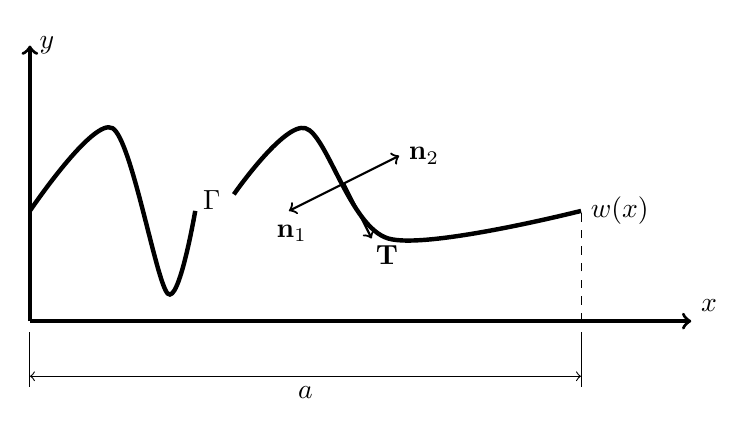
\begin{tikzpicture}[scale=0.7]
		\draw [ultra thick] plot [smooth] coordinates {(0, 2) (1.5, 3.5) (2.5, 0.5) (3, 2)};
		\draw [ultra thick] plot [smooth] coordinates {(3.7, 2.3) (5, 3.5) (6.5, 1.5) (10, 2)};		
		\draw [dashed] (10, 0) -- (10, 2);
		
		\draw (3.3, 2.2) node {$\Gamma$};
		\draw (5, -1.3) node {$a$};
		
		\node [above right] at (12, 0) {$x$};
		\node [right] at (0, 5) {$y$};
		
		\draw [->, thick] (5.7,2.5) -- (4.7,2);
		\node [right] at (4.3, 1.6) {$\mathbf{n}_1$};
		
		\draw [->, thick] (5.7,2.5) -- (6.7,3);
		\node [right] at (6.7, 3) {$\mathbf{n}_2$};
		
		\draw [->, thick] (5.7,2.5) -- (6.2,1.5);
		\node [right] at (6.1, 1.2) {$\mathbf{T}$};
		
		\node [right] at (10, 2) {$w(x)$};
		
		\draw [->, very thick] (0,0) -- (12,0);
		\draw [->, very thick] (0, 0) -- (0,5);
		
		\draw [-] (0, -0.2) -- (0, -1.2);
		\draw [-] (10, -0.2) -- (10, -1.2);
		\draw [<->] (0, -1) -- (10, -1);
		\end{tikzpicture}
		\caption{Vetores normais e tangente à interface $\Gamma$}
		\label{fig7}
	\end{center}
\end{figure}

A curva que representa $\Gamma$ pode ser escrita de forma paramétrica como segue:
\begin{align}
\Gamma(t) = x(t) \mathbf{a}_x + y(t) \mathbf{a}_y, \quad 0 \le t \le a \label{forma_parametrica}
\end{align}
onde $\mathbf{a}_x$ e $\mathbf{a}_y$ são os vetores unitários da base canônica do sistema cartesiano.

A parametrização a ser adotada será:
\begin{align}
& x(t) = t \label{parametrizacao_x}\\
& y(t) = w(t) \label{parametrizacao_y}
\end{align}

Substituindo em \eqref{forma_parametrica}, obtém-se:
\begin{align}
\Gamma(t) = t \mathbf{a}_x + w(t) \mathbf{a}_y \label{forma_parametrica_substituida}
\end{align}

O vetor tangente unitário $\mathbf{T}$ será dado por \citep{livro_stewart_2}:
\begin{align}
& \mathbf{T}(t) = \frac{\Gamma'(t)}{\norm{\Gamma'(t)}} \nonumber \\
& \Rightarrow \mathbf{T}(t) = \frac{\mathbf{a}_x + w'(t) \mathbf{a}_y}{\sqrt{1 + w'(t)^2}}
\end{align}

O vetor normal unitário principal $\mathbf{N}$ será dado por \citep{livro_stewart_2}:
\begin{align}
& \mathbf{N}(t) = \frac{\mathbf{T}'(t)}{\norm{\mathbf{T}'(t)}} \nonumber \\
& \Rightarrow \mathbf{N}(t) = \frac{ \displaystyle\frac{d}{dt}\left[\frac{1}{\sqrt{1 + w'(t)^2}}\right]\mathbf{a}_x
	+
	\displaystyle\frac{d}{dt}\left[\frac{w'(t)}{\sqrt{1 + w'(t)^2}}\right]\mathbf{a}_y }
{\sqrt{ \left\lbrace \displaystyle\frac{d}{dt}\left[\frac{1}{\sqrt{1 + w'(t)^2}}\right] \right\rbrace ^2
		+
		\left\lbrace \displaystyle\frac{d}{dt}\left[\frac{w'(t)}{\sqrt{1 + w'(t)^2}}\right] \right\rbrace ^2 }} \nonumber \\
& \Rightarrow \mathbf{N}(t) = \frac{ -\displaystyle \frac{w'(t)w''(t)}{[1 + w'(t)^2]^{3/2}} \mathbf{a}_x
	+
	\displaystyle \frac{w''(t)}{[1 + w'(t)^2]^{3/2}} \mathbf{a}_y }
{\sqrt{ \displaystyle \frac{w'(t)^2 w''(t)^2}{[1 + w'(t)^2]^3} 
		+
		\displaystyle \frac{w''(t)^2}{[1 + w'(t)^2]^{3}} }} \nonumber \\
& \Rightarrow \mathbf{N}(t) = \frac{ \displaystyle\frac{w''(t)}{[1 + w'(t)^2]^{3/2}} [-w'(t)\mathbf{a}_x + \mathbf{a}_y] }
{\sqrt{ \displaystyle \frac{w''(t)^2}{[1 + w'(t)^2]^3} [w'(t)^2	+ 1] }} \nonumber \\
& \Rightarrow \mathbf{N}(t) = \frac{w''(t)}{\abs{w''(t)}} \frac{ -w'(t)\mathbf{a}_x + \mathbf{a}_y }
{\sqrt{ 1 + w'(t)^2 }} \nonumber \\
& \Rightarrow \mathbf{N}(t) = \left\lbrace\begin{array}{ll}
\displaystyle\frac{ -w'(t)\mathbf{a}_x + \mathbf{a}_y}{\sqrt{ 1 + w'(t)^2 }}, & w''(t) > 0 \\ \\
\displaystyle\frac{ w'(t)\mathbf{a}_x - \mathbf{a}_y}{\sqrt{ 1 + w'(t)^2 }}, & w''(t) < 0
\end{array}\right.
\label{equacao_normal_geometria_diferencial}
\end{align}

Uma característica do vetor normal principal é que ele sempre aponta para a parte côncava da superfície. Retornando à figura \ref{fig7}, pode-se observar que no ponto de exemplo onde os vetores unitários foram representados, o vetor unitário $\mathbf{n}_1$ é o que corresponde ao vetor normal principal. Como a concavidade neste ponto está voltada para baixo, a segunda derivada da equação que representa a superfície terá sinal negativo \cite{livro_stewart_1}, ou seja, $w''(t) \equiv w''(x) < 0$, logo, pela equação \eqref{equacao_normal_geometria_diferencial}:
\begin{align}
\mathbf{n}_1 = \frac{ w'(x)\mathbf{a}_x - \mathbf{a}_y }{\sqrt{ 1 + w'(x)^2 }} \label{equacao_normal_geometria_diferencial_1}
\end{align}
onde a variável paramétrica $t$ foi substituída por $x$, uma vez que são equivalentes.

A expressão para $\mathbf{n}_2$ é imediata, já que aponta para o sentido oposto ao de $\mathbf{n}_1$:
\begin{align}
\mathbf{n}_2 = \frac{ -w'(x)\mathbf{a}_x + \mathbf{a}_y }{\sqrt{ 1 + w'(x)^2 }} \label{equacao_normal_geometria_diferencial_2}
\end{align}

Nos trechos em que a concavidade está voltada para cima, a normal principal corresponderá a $\mathbf{n}_2$; como $w''(x) > 0$ nesses trechos, a expressão para $\mathbf{n}_2$ continuará sendo \eqref{equacao_normal_geometria_diferencial_2}. Assim, as equações \eqref{equacao_normal_geometria_diferencial_1} e \eqref{equacao_normal_geometria_diferencial_2} representam respectivamente os vetores normais $\mathbf{n}_1$ e $\mathbf{n}_2$ em qualquer ponto da superfície $\Gamma$.




Desse modo, aplicando a equação \eqref{derivada_direcional_coodernadas_cartesianas} para o vetor unitário $\mathbf{n}_1$, obtém-se a derivada do campo escalar $\Phi$
em relação a esse vetor, em coordenadas cartesianas: 
\begin{align}
& \frac{\partial\Phi}{\partial\mathbf{n_1}} = \frac{1}{\sqrt{1 + w'(x)^2}}\left[w'(x)\frac{\partial \Phi}{\partial x} - \frac{\partial \Phi}{\partial y}\right]
\label{derivada_direcional_para_n1}
\end{align} 
e, em relação ao vetor $\mathbf{n}_2$:
\begin{align}
& \frac{\partial\Phi}{\partial\mathbf{n_2}} = -\frac{1}{\sqrt{1 + w'(x)^2}}\left[w'(x)\frac{\partial \Phi}{\partial x} - \frac{\partial \Phi}{\partial y}\right]
\label{derivada_direcional_para_n2}
\end{align} 

Tomando como exemplo a condição de contorno \eqref{funcao_F_cc_T1_5}, e aplicando as expressões \eqref{derivada_direcional_para_n1} e \eqref{derivada_direcional_para_n2},
a fim de escrever esta condição em coordenadas cartesianas,
tem-se:
\begin{align}
& k_2\frac{\partial F_{2, j}}{\partial\mathbf{n}_2} = - k_1\frac{\partial F_{1,j}}{\partial\mathbf{n}_1} \nonumber \\
& \Rightarrow -\frac{k_2}{\sqrt{1 + w'(x)^2}}\left[w'(x)\frac{\partial F_{2,j}(x, w(x))}{\partial x} - \frac{\partial F_{2,j}(x, w(x))}{\partial y}\right] = \nonumber \\
& -\frac{k_1}{\sqrt{1 + w'(x)^2}}\left[w'(x)\frac{\partial F_{1,j}(x, w(x))}{\partial x} - \frac{\partial F_{1,j}(x, w(x))}{\partial y}\right] \nonumber \\
& \Rightarrow k_2\left[w'(x)\frac{\partial F_{2,j}(x, w(x))}{\partial x} - \frac{\partial F_{2,j}(x, w(x))}{\partial y}\right] = \nonumber \\
& k_1 \left[w'(x)\frac{\partial F_{1,j}(x, w(x))}{\partial x} - \frac{\partial F_{1,j}(x, w(x))}{\partial y}\right]
\end{align}

\subsubsection{Formulação dos problemas auxiliares no sistema cartesiano: domínio físico original}

Reescrevendo-se o primeiro problema auxiliar em coordenadas cartesianas, empregando os resultados encontrados na seção \ref{secao_sobre_normal}, obtém-se o sistema de equações a seguir:
\begin{subequations}
	\begin{alignat}{2}
	& \frac{\partial^2 F_{1,j}(x, y)}{\partial x^2} + \frac{\partial^2 F_{1,j}(x, y)}{\partial y^2} = 0  && 0 < x < a, w(x) < y < b \label{funcao_F_harm_T1_cart} \\ \nonumber \\
	& F_{1,j}(x, b) = \psi_j(x) && 0 < x < a  \label{funcao_F_cc_T1_2_cart} \\ \nonumber \\
	& \frac{\partial F_{1,j}(0, y)}{\partial x} = 0 && w(0) < y < b \label{funcao_F_cc_T1_1a_cart} \\ \nonumber \\
	& \frac{\partial F_{1,j}(a, y)}{\partial x} = 0 && w(a) < y < b \label{funcao_F_cc_T1_1b_cart} \\ \nonumber \\
	& F_{1,j}(x, w(x)) = F_{2, j}(x, w(x)) && 0 < x < a \label{funcao_F_cc_grad_T1_cart} \\ \nonumber \\
	& \frac{\partial^2 F_{2,j}(x, y)}{\partial x^2} + \frac{\partial^2 F_{2,j}(x, y)}{\partial y^2} = 0 &&  0 < x < a, 0 < y < w(x) \label{funcao_F_harm_T2_cart} \\ \nonumber \\
	& \frac{\partial F_{2,j}(0, y)}{\partial x} = 0 && 0 < y < w(0) \label{funcao_F_cc_T1_3a_cart} \\ \nonumber \\
	& \frac{\partial F_{2,j}(a, y)}{\partial x} = 0 && 0 < y < w(a) \label{funcao_F_cc_T1_3b_cart} \\ \nonumber \\
	& F_{2,j}(x, 0) = 0 && 0 < x < a \label{funcao_F_cc_T1_4_cart} \\ \nonumber \\
	& k_2\left[w'(x)\frac{\partial F_{2,j}(x, w(x))}{\partial x} - \frac{\partial F_{2,j}(x, w(x))}{\partial y}\right] = \nonumber \\
	& k_1\left[w'(x)\frac{\partial F_{1,j}(x, w(x))}{\partial x} - \frac{\partial F_{1,j}(x, w(x))}{\partial y}\right] && 0 < x < a \label{funcao_F_cc_T1_5_cart}
	\end{alignat}
\end{subequations}

Já o segundo problema auxiliar assume a forma:
\begin{subequations}
	\begin{alignat}{2}
	& \frac{\partial^2 G_{1,j}(x, y)}{\partial x^2} + \frac{\partial^2 G_{1,j}(x, y)}{\partial y^2} = 0 \quad\quad && 0 < x < a, w(x) < y < b \label{funcao_G_harm_T1_cart} \\ \nonumber \\
	& G_{1,j}(x, b) = \phi_j(x) && 0 < x < a  \label{funcao_G_cc_T1_2_cart} \\ \nonumber \\
	& \frac{\partial G_{1,j}(0, y)}{\partial x} = 0 && w(0) < y < b \label{funcao_G_cc_T1_1a_cart} \\ \nonumber \\
	& \frac{\partial G_{1,j}(a, y)}{\partial x} = 0 && w(a) < y < b \label{funcao_G_cc_T1_1b_cart} \\ \nonumber \\
	& w'(x)\frac{\partial G_{1,j}(x, w(x))}{\partial x} - \frac{\partial G_{1,j}(x, w(x))}{\partial y} = 0 \quad\quad\quad && 0 < x < a \label{funcao_G_cc_grad_T1_cart}
	\end{alignat}
\end{subequations}

\subsubsection{Extensão dos domínios dos problemas auxiliares no sistema cartesiano}\label{secao_formulacao_aux}

Os problemas associados às funções auxiliares $F_{1,j}$ e $G_{1,j}$ devem ser resolvidos na região definida por $0 \le x \le a, w(x) \le y \le b$, ao passo que o problema associado à função auxiliar $F_{2,j}$ deve ser resolvido na região definida por $0 \le x \le a, 0 \le y \le w(x)$. Estas regiões, ou subdomínios, delimitados pelas regiões $\Omega_1$ e $\Omega_2$, e separados pela interface $\Gamma$, dificultam o emprego direto da CITT em coordenadas
cartesianas, uma vez que aquela interface tem um formato irregular que aumenta a complexidade da aplicação da separação de variáveis na formulação dos problemas
de autovalor associado.

A fim de contornar essa dificuldade, será feita uma \textit{extensão} dos subdomínios $\Omega_1$ e $\Omega_2$, gerando dois novos domínios retangulares,
que envolverão respectivamente os subdomínios originais e que efetivamente coincidirão com o domínio maior $\Omega$, delimitado pela região $0 \le x \le a, 0 \le y \le b$. Os problemas auxiliares originais serão válidos para esses novos domínios, de forma a ainda
satisfazerem as condições de contorno dos subdomínios originais.
Desse modo, as soluções analíticas das funções $F_{1, j}$ e $G_{1, j}$ serão obtidas a partir do domínio estendido representado na figura \ref{fig5}, enquanto que
as soluções analíticas das funções $F_{2, j}$ serão obtidas a partir do domínio estendido representado na figura \ref{fig6}.

\begin{figure}[H]
	\begin{center}
		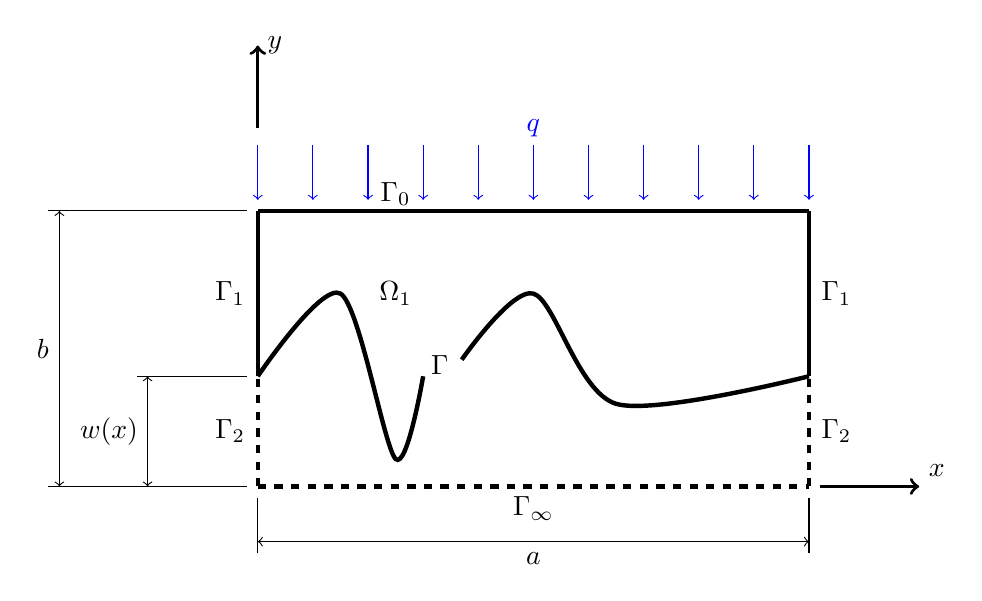
\begin{tikzpicture}[scale=0.7]
		
		\draw [ultra thick, dashed] (0, 0) -- (10, 0);
		%\draw [ultra thick] (0, 2) -- (7, 2);
		%\draw [ultra thick] (8, 2) -- (10, 2);
		\draw [ultra thick] plot [smooth] coordinates {(0, 2) (1.5, 3.5) (2.5, 0.5) (3, 2)};
		\draw [ultra thick] plot [smooth] coordinates {(3.7, 2.3) (5, 3.5) (6.5, 1.5) (10, 2)};
		\draw [ultra thick] (0, 5) -- (10, 5);
		\draw [ultra thick, dashed] (0, 0) -- (0, 2);	
		\draw [ultra thick] (0, 2) -- (0, 5);	
		\draw [ultra thick, dashed] (10, 0) -- (10, 2);
		\draw [ultra thick] (10, 2) -- (10, 5);
		
		\draw (2.5, 3.5) node {$\Omega_1$};
		\draw (3.3, 2.2) node {$\Gamma$};
		\draw (-0.5, 3.5) node {$\Gamma_1$};
		\draw (-0.5, 1) node {$\Gamma_2$};
		\draw (10.5, 3.5) node {$\Gamma_1$};
		\draw (10.5, 1) node {$\Gamma_2$};
		\draw (5, -0.4) node {$\Gamma_\infty$};
		\draw (2.5, 5.3) node {$\Gamma_0$};
		\draw [blue](5, 6.5) node {$q$};
		\draw (5, -1.3) node {$a$};
		\draw (-3.9, 2.5) node {$b$};
		\draw (-2.7, 1) node {$w(x)$};
		
		\node [above right] at (12, 0) {$x$};
		\node [right] at (0, 8) {$y$};
		
		\draw [->, blue] (0, 6.2) -- (0, 5.2);
		\draw [->, blue] (1, 6.2) -- (1, 5.2);
		\draw [->, blue] (2, 6.2) -- (2, 5.2);
		\draw [->, blue] (3, 6.2) -- (3, 5.2);
		\draw [->, blue] (4, 6.2) -- (4, 5.2);
		\draw [->, blue] (5, 6.2) -- (5, 5.2);
		\draw [->, blue] (6, 6.2) -- (6, 5.2);
		\draw [->, blue] (7, 6.2) -- (7, 5.2);
		\draw [->, blue] (8, 6.2) -- (8, 5.2);
		\draw [->, blue] (9, 6.2) -- (9, 5.2);
		\draw [->, blue] (10, 6.2) -- (10, 5.2);
		
		\draw [->, very thick] (10.2,0) -- (12,0);
		\draw [->, very thick] (0, 6.5) -- (0,8);
		
		\draw [-] (0, -0.2) -- (0, -1.2);
		\draw [-] (10, -0.2) -- (10, -1.2);
		\draw [<->] (0, -1) -- (10, -1);
		
		\draw [-] (-0.2, 0) -- (-3.8, 0);
		\draw [-] (-0.2, 5) -- (-3.8, 5);
		\draw [-] (-0.2, 2) -- (-2.2, 2);
		\draw [<->] (-3.6, 0) -- (-3.6, 5);
		\draw [<->] (-2.0, 0) -- (-2.0, 2);
		
		\end{tikzpicture}
		\caption{Extensão do subdomínio $\Omega_1$ para as funções $F_{1, j}$ e $G_{1, j}$}
		\label{fig5}
	\end{center}
\end{figure}

\begin{figure}[H]
	\begin{center}
		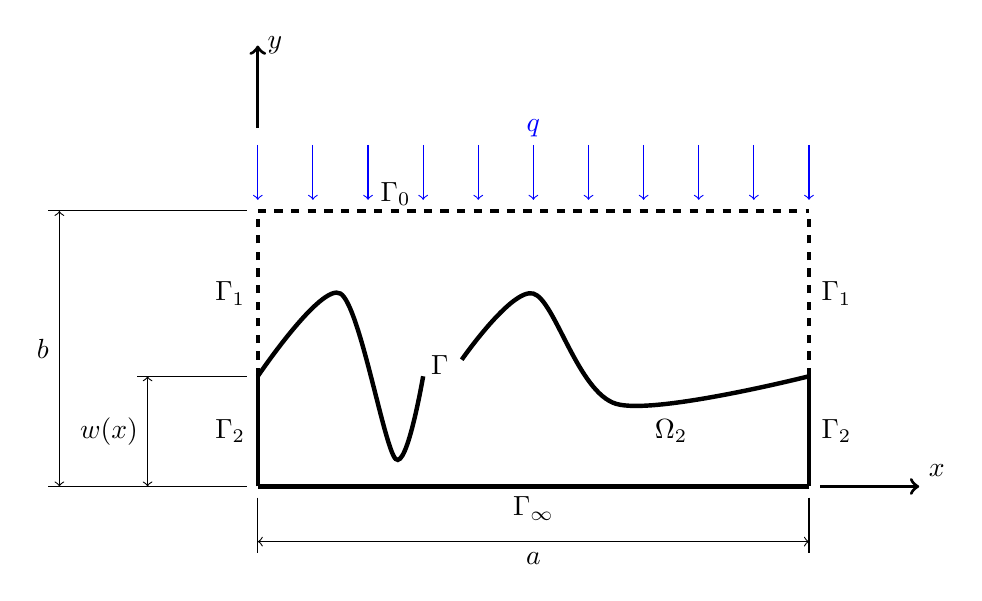
\begin{tikzpicture}[scale=0.7]
		
		\draw [ultra thick] (0, 0) -- (10, 0);
		%\draw [ultra thick] (0, 2) -- (7, 2);
		%\draw [ultra thick] (8, 2) -- (10, 2);
		\draw [ultra thick] plot [smooth] coordinates {(0, 2) (1.5, 3.5) (2.5, 0.5) (3, 2)};
		\draw [ultra thick] plot [smooth] coordinates {(3.7, 2.3) (5, 3.5) (6.5, 1.5) (10, 2)};
		\draw [ultra thick, dashed] (0, 5) -- (10, 5);
		\draw [ultra thick] (0, 0) -- (0, 2);	
		\draw [ultra thick, dashed] (0, 2) -- (0, 5);	
		\draw [ultra thick] (10, 0) -- (10, 2);
		\draw [ultra thick, dashed] (10, 2) -- (10, 5);
		
		\draw (7.5, 1) node {$\Omega_2$};	
		\draw (3.3, 2.2) node {$\Gamma$};
		\draw (-0.5, 3.5) node {$\Gamma_1$};
		\draw (-0.5, 1) node {$\Gamma_2$};
		\draw (10.5, 3.5) node {$\Gamma_1$};
		\draw (10.5, 1) node {$\Gamma_2$};
		\draw (5, -0.4) node {$\Gamma_\infty$};
		\draw (2.5, 5.3) node {$\Gamma_0$};
		\draw [blue](5, 6.5) node {$q$};
		\draw (5, -1.3) node {$a$};
		\draw (-3.9, 2.5) node {$b$};
		\draw (-2.7, 1) node {$w(x)$};
		
		\node [above right] at (12, 0) {$x$};
		\node [right] at (0, 8) {$y$};
		
		\draw [->, blue] (0, 6.2) -- (0, 5.2);
		\draw [->, blue] (1, 6.2) -- (1, 5.2);
		\draw [->, blue] (2, 6.2) -- (2, 5.2);
		\draw [->, blue] (3, 6.2) -- (3, 5.2);
		\draw [->, blue] (4, 6.2) -- (4, 5.2);
		\draw [->, blue] (5, 6.2) -- (5, 5.2);
		\draw [->, blue] (6, 6.2) -- (6, 5.2);
		\draw [->, blue] (7, 6.2) -- (7, 5.2);
		\draw [->, blue] (8, 6.2) -- (8, 5.2);
		\draw [->, blue] (9, 6.2) -- (9, 5.2);
		\draw [->, blue] (10, 6.2) -- (10, 5.2);
		
		\draw [->, very thick] (10.2,0) -- (12,0);
		\draw [->, very thick] (0, 6.5) -- (0,8);
		
		\draw [-] (0, -0.2) -- (0, -1.2);
		\draw [-] (10, -0.2) -- (10, -1.2);
		\draw [<->] (0, -1) -- (10, -1);
		
		\draw [-] (-0.2, 0) -- (-3.8, 0);
		\draw [-] (-0.2, 5) -- (-3.8, 5);
		\draw [-] (-0.2, 2) -- (-2.2, 2);
		\draw [<->] (-3.6, 0) -- (-3.6, 5);
		\draw [<->] (-2.0, 0) -- (-2.0, 2);
		
		\end{tikzpicture}
		\caption{Extensão do subdomínio $\Omega_2$ para as funções $F_{2, j}$}
		\label{fig6}
	\end{center}
\end{figure}

\subsection{Solução analítica dos problemas auxiliares através da Técnica da Transformada Integral Clássica}

\subsubsection{Problema homogêneo de autovalor associado ao primeiro problema auxiliar}

As condições de contorno \eqref{funcao_F_cc_T1_1a_cart} e \eqref{funcao_F_cc_T1_1b_cart}, na direção $x$, referentes ao problema de valor de contorno das funções $F_{1, j}$, são homogêneas e de segundo tipo. O
mesmo pode ser observado nas condições de contorno \eqref{funcao_F_cc_T1_3a_cart} e \eqref{funcao_F_cc_T1_3b_cart}, na direção $x$, referentes ao problema de valor de contorno das funções $F_{2, j}$.
Assim, o problema de autovalor associado, ou de Sturm-Liouville, será o mesmo para os dois problemas auxiliares:
\begin{subequations}
	\begin{alignat}{2}
	& \frac{d^2 X(\mu_m, x)}{d x^2} + \mu_m^2 X(\mu_m, x) = 0 \quad\quad\quad\quad\quad\quad && 0 < x < a \label{problema_vc_1a} \\ \nonumber \\
	& \frac{d X(\mu_m, x)}{d x} = 0 && x = 0 \label{problema_vc_1b} \\ \nonumber \\
	& \frac{d X(\mu_m, x)}{d x} = 0 && x = a \label{problema_vc_1c}
	\end{alignat}
\end{subequations}
onde $\mu_m$ são os autovalores e $X(\mu_m, x)$ são as autofunções correspondentes. Resolvendo-se o problema de autovalor definido em \eqref{problema_vc_1a}--\eqref{problema_vc_1c}, obtém-se \citep{livro_ozisik}:
\begin{align}
& X(\mu_m, x) = \left\lbrace
\begin{array}{ll}
1, & m = 0 \\ \\
\cos \mu_m x, & m = 1,2,3,\ldots
\end{array}
\right . \label{definicao_das_autofuncoes} \\ \nonumber \\
& N(\mu_m) = \left\lbrace
\begin{array}{ll}
a, \quad\quad\quad\quad & m = 0 \\ \\
\displaystyle\frac{a}{2}, & m = 1,2,3,\ldots
\end{array}
\right. \label{valor_integral_norm}
\end{align}
onde $N(\mu_m)$ é denominada integral de normalização, definida por
\begin{align}
N(\mu_m) = \int_0^a X(\mu_m, x)^2 dx
\end{align}

Os autovalores $\mu_m$ são dados por:
\begin{align}
\mu_m = \left\lbrace
\begin{array}{ll}
0, \quad\quad\quad\quad & m = 0 \\ \\
\displaystyle\frac{m\pi}{a}, & m = 1,2,3,\ldots
\end{array}
\right.
\end{align}

As autofunções $X(\mu_m, x), m=0,1,2,3,\ldots$, do problema de autovalor \eqref{problema_vc_1a}--\eqref{problema_vc_1c}, atendem à condição de ortogonalidade:
\begin{align}
& \int_0^a X(\mu_m, x)X(\mu_n, x)dx 
= \left\lbrace
\begin{array}{ll}
0 \quad\quad\quad\quad & \text{para  } m \neq n \\ \\
N(\mu_m) & \text{para  }m = n
\end{array}
\right. \label{ortogon}
\end{align}

\subsubsection{Definição do par transformada-inversa associado ao primeiro problema auxiliar}

Considera-se agora que tanto $F_{1, j}$ quanto $F_{2, j}$ possam ser representados em termos das autofunções $X(\mu_m, x)$ como segue:
\begin{align}
& F_{1, j}(x, y) = \sum_{m=0}^\infty C_{j,m}(y)X(\mu_m, x) \label{expansao_para_F1}\\ \nonumber \\
& F_{2, j}(x, y) = \sum_{m=0}^\infty D_{j,m}(y)X(\mu_m, x) \label{expansao_para_F2}
\end{align}

Os coeficientes $C_{j,m}(y)$ e $D_{j,m}(y)$ podem ser determinados através da aplicação da propriedade de ortogonalidade expressa em \eqref{ortogon}. Assim, multiplicando as equações
\eqref{expansao_para_F1} e \eqref{expansao_para_F2} por $X(\mu_n, x)$ e integrando em relação a $x$ no intervalo $0 < x < a$, obtém-se:
\begin{align}
& \int_0^a F_{1, j}(x, y)X(\mu_n, x)dx = \sum_{m=0}^\infty C_{j,m}(y) \int_0^a X(\mu_m, x)X(\mu_n, x)dx \label{somatorio_para_F1}\\ \nonumber \\
& \int_0^a F_{2, j}(x, y)X(\mu_n, x)dx = \sum_{m=0}^\infty D_{j,m}(y) \int_0^a X(\mu_m, x)X(\mu_n, x)dx \label{somatorio_para_F2}
\end{align}

As integrais acima, de acordo com a propriedade de ortogonalidade, anulam-se quando $m \ne n$, e são iguais a $N(\mu_m)$ quando $m = n$. Assim, cada somatório se reduz apenas ao
termo de índice $m$, de modo que os coeficientes serão dados por:
\begin{align}
& C_{j,m}(y) = \frac{1}{N(\mu_m)}\int_0^a F_{1, j}(x, y)X(\mu_m, x)dx \label{coef_para_F1}\\ \nonumber \\
& D_{j,m}(y) = \frac{1}{N(\mu_m)}\int_0^a F_{2, j}(x, y)X(\mu_m, x)dx \label{coef_para_F2}
\end{align}

Substituindo as relações \eqref{coef_para_F1} e \eqref{coef_para_F2} nos somatórios \eqref{expansao_para_F1} e \eqref{expansao_para_F2}, respectivamente, obtém-se:
\begin{align}
& F_{1, j}(x, y) = \sum_{m=0}^\infty \frac{X(\mu_m, x)}{N(\mu_m)}\int_0^a F_{1, j}(x', y)X(\mu_m, x')dx' \label{expansao_para_F1_nova}\\ \nonumber \\
& F_{2, j}(x, y) = \sum_{m=0}^\infty \frac{X(\mu_m, x)}{N(\mu_m)}\int_0^a F_{2, j}(x', y)X(\mu_m, x')dx' \label{expansao_para_F2_nova}
\end{align}

Denota-se a \textit{transformada integral} de $F_{1, j}$ e $F_{2, j}$ na direção $x$ respectivamente por $\bar{F}_{1,j,m}(y)$ e $\bar{F}_{2,j,m}(y)$.
Desse modo, cada uma das expressões acima pode ser dividida em duas partes, definindo o par \textit{transformada-inversa} para as funções $F_{1,j}$ e $F_{2,j}$:
\begin{itemize}
	\item Funções $F_{1, j}$:
	\begin{fleqn}
		\begin{alignat}{2}
		& \text{Inversa:} && F_{1, j}(x, y) = \sum_{m=0}^\infty \frac{X(\mu_m, x)}{N(\mu_m)}\bar{F}_{1,j,m}(y) \label{definicao_da_transf_inv_F1} \\ \nonumber \\
		& \text{Transformada:} \quad\quad && \bar{F}_{1,j,m}(y) = \int_0^a F_{1, j}(x, y) X(\mu_m, x) dx \label{definicao_da_transf_F1}
		\end{alignat}
	\end{fleqn}
	\item Funções $F_{2, j}$:
	\begin{fleqn}
		\begin{alignat}{2}
		& \text{Inversa:} && F_{2, j}(x, y) = \sum_{m=0}^\infty \frac{X(\mu_m, x)}{N(\mu_m)}\bar{F}_{2,j,m}(y) \label{definicao_da_transf_inv_F2} \\ \nonumber \\
		& \text{Transformada:} \quad\quad && \bar{F}_{2,j,m}(y) = \int_0^a F_{2, j}(x, y) X(\mu_m, x) dx
		\label{definicao_da_transf_F2}
		\end{alignat}
	\end{fleqn}
\end{itemize}

\subsubsection{Aplicação da transformação integral às equações do primeiro problema auxiliar}\label{secao_reciprocidade_F}

Uma vez definidos os pares transformada-inversa para as funções $F_{1,j}$ e $F_{2,j}$, procede-se à transformação integral na direção $x$ das equações
diferenciais parciais \eqref{funcao_F_harm_T1_cart} e \eqref{funcao_F_harm_T2_cart}, obtendo-se equações diferenciais ordinárias em $y$ envolvendo
as funções transformadas $\bar{F}_{1,j,m}(y)$ e $\bar{F}_{2,j,m}(y)$. Este procedimento será realizado inicialmente para a equação \eqref{funcao_F_harm_T1_cart};
os resultados serão análogos para a equação \eqref{funcao_F_harm_T2_cart}.

Multiplicando-se então a equação \eqref{funcao_F_harm_T1_cart} por $X(\mu_m, x)$ e integrando em relação a $x$ no intervalo $0 < x < a$, obtemos: 
\begin{align}
& \int_0^a  \frac{\partial^2 F_{1,j}(x, y)}{\partial x^2}X(\mu_m, x)dx + \int_0^a \frac{\partial^2 F_{1,j}(x, y)}{\partial y^2}X(\mu_m, x)dx = 0 
\end{align}

Na expressão acima, a primeira integral pode ser desenvolvida através de integração por partes, enquanto que na segunda integral, os operadores de derivada
em relação a $y$ e integração em relação a $x$ podem ser permutados:
\begin{align}
& \left[ \frac{\partial F_{1,j}(x, y)}{\partial x}X(\mu_m, x) \right]_0^a
-
\int_0^a  \frac{\partial F_{1,j}(x, y)}{\partial x}\frac{dX(\mu_m, x)}{dx} dx + \nonumber \\
& \frac{d^2}{d y^2}\int_0^a F_{1,j}(x, y)X(\mu_m, x)dx = 0 \nonumber \\ 
\Rightarrow & \frac{\partial F_{1,j}(a, y)}{\partial x}X(\mu_m, a) - \frac{\partial F_{1,j}(0, y)}{\partial x}X(\mu_m, 0)
-
\int_0^a  \frac{\partial F_{1,j}(x, y)}{\partial x}\frac{dX(\mu_m, x)}{dx} dx + \nonumber \\
& \frac{d^2}{d y^2}\int_0^a F_{1,j}(x, y)X(\mu_m, x)dx = 0
\end{align}

As condições de contorno \eqref{funcao_F_cc_T1_1a_cart} e \eqref{funcao_F_cc_T1_1b_cart} anulam os dois primeiros termos da expressão acima. A primeira
integral também pode ser desenvolvida por partes. A segunda integral é exatamente a transformada integral da função $F_{1, j}$, conforme a equação \eqref{definicao_da_transf_F1}.
Assim:
\begin{align}
&
- \left[ F_{1,j}(x, y)\frac{dX(\mu_m, x)}{dx} \right]_0^a
+ \int_0^a  F_{1,j}(x, y)\frac{d^2X(\mu_m, x)}{dx^2} dx + \frac{d^2 \bar{F}_{1,j,m}(y)}{d y^2} = 0 \nonumber \\
\Rightarrow &
- F_{1,j}(a, y)\frac{dX(\mu_m, a)}{dx}+ F_{1,j}(0, y)\frac{dX(\mu_m, 0)}{dx} + \int_0^a  F_{1,j}(x, y)\frac{d^2X(\mu_m, x)}{dx^2} dx + \nonumber \\
& \frac{d^2 \bar{F}_{1,j,m}(y)}{d y^2} = 0
\end{align}

Aplicando as condições de contorno \eqref{problema_vc_1b} e \eqref{problema_vc_1c}, a expressão resulta em: 
\begin{align}
&
\int_0^a  F_{1,j}(x, y)\frac{d^2X(\mu_m, x)}{dx^2} dx + \frac{d^2 \bar{F}_{1,j,m}(y)}{d y^2} = 0 \label{equacao_intermediaria_F1}
\end{align}

Da equação do problema homogêneo de autovalor associado \eqref{problema_vc_1a}, obtém-se:
\begin{align}
\frac{d^2 X(\mu_m, x)}{d x^2} = -\mu_m^2 X(\mu_m, x) \label{substituicao_autofuncao}
\end{align}

A substituição de \eqref{substituicao_autofuncao} em \eqref{equacao_intermediaria_F1} resulta em:
\begin{align}
&
\int_0^a  F_{1,j}(x, y)[-\mu_m^2 X(\mu_m, x)] dx + \frac{\partial^2 \bar{F}_{1,j,m}(y)}{\partial y^2} = 0 \nonumber \\
\Rightarrow &
\frac{d^2 \bar{F}_{1,j,m}(y)}{d y^2}
-
\mu_m^2 \int_0^a  F_{1,j}(x, y)X(\mu_m, x) dx = 0
\end{align}

Finalmente, aplicando a definição da transformada integral de $F_{1, j}$, obtém-se uma equação diferencial ordinária para $\bar{F}_{1,j,m}(y)$:
\begin{align}
\frac{d^2 \bar{F}_{1,j,m}(y)}{d y^2}
-
\mu_m^2 \bar{F}_{1,j,m}(y) = 0 \label{eq_dif_ord_F1}
\end{align}

Seguindo o mesmo procedimento para a equação \eqref{funcao_F_harm_T2_cart}, obtém-se uma equação diferencial ordinária para $\bar{F}_{2,j,m}(y)$:
\begin{align}
\frac{d^2 \bar{F}_{2,j,m}(y)}{d y^2}
-
\mu_m^2 \bar{F}_{2,j,m}(y) = 0 \label{eq_dif_ord_F2}
\end{align}

Neste ponto justifica-se o emprego do recurso da extensão de domínio (cf. secão \ref{secao_formulacao_aux}): a aplicação da transformação integral em $x$ às equações diferenciais parciais originais do problema eliminou a dependência em $x$, fornecendo assim as equações diferenciais ordinárias \eqref{eq_dif_ord_F1} e \eqref{eq_dif_ord_F2}, dependentes apenas de $y$. Se estas equações fossem resolvidas respectivamente para os domínios $w(x) < y < b$ e $0 < y < w(x)$, a variável $x$ seria reintroduzida, trazendo dificuldades na busca da solução, o que não acontece quando se adota o domínio $0 < y < b$ para resolução de ambas as equações. Nessas condições, as equações diferenciais \eqref{eq_dif_ord_F1} e \eqref{eq_dif_ord_F2} admitem as seguintes soluções fundamentais \citep{livro_boyce}:
\begin{align}
& f_{1,j,m}(y) = \sinh\mu_m y \label{basic_1}\\ \nonumber \\
& g_{1,j,m}(y) = \cosh\mu_m y \label{basic_2}
\end{align}

As soluções gerais das equações \eqref{eq_dif_ord_F1} e \eqref{eq_dif_ord_F2} serão então dadas pela combinação linear destas funções, que podem ser escritas na forma:
\begin{align}
& \bar{F}_{1,j,m}(y) = \mathbb{A}_{j,m}\frac{\sinh\mu_m (b - y)}{\sinh\mu_m b} + \mathbb{B}_{j,m}\frac{\sinh\mu_m y}{\sinh\mu_m b} \label{solucao_temporaria_F1}\\ \nonumber \\
& \bar{F}_{2,j,m}(y) = \mathbb{C}_{j,m}\frac{\sinh\mu_m (b - y)}{\sinh\mu_m b} + \mathbb{D}_{j,m}\frac{\sinh\mu_m y}{\sinh\mu_m b} \label{solucao_temporaria_F2}
\end{align} 
onde $\mathbb{A}_{j,m}, \mathbb{B}_{j,m}, \mathbb{C}_{j,m}$ e $\mathbb{D}_{j,m}$ são constantes a determinar\footnote{A expressão \eqref{solucao_temporaria_F1}, através da expansão dos argumentos das funções hiberbólicas, pode ser reescrita como:
	
	\begin{align*}
	& \bar{F}_{1,j,m}(y) = \left( \frac{\mathbb{B}_{j,m} - \mathbb{A}_{j,m} \cosh\mu_m b}{\sinh\mu_m b}\right)\sinh\mu_m y + \frac{\mathbb{A}_{j,m}\sinh\mu_m b}{\sinh\mu_m b}\cosh\mu_m y
	\end{align*}	
	que é uma combinação linear das soluções \eqref{basic_1} e \eqref{basic_2}; observações semelhantes podem ser feitas para a expressões \eqref{solucao_temporaria_F2}, \eqref{solucao_temporaria_F1_0} e \eqref{solucao_temporaria_F2_0}. Essa forma de expressar as soluções facilitará a determinação dos coeficientes $\mathbb{A}_{j,m}$, $\mathbb{B}_{j,m}$, $\mathbb{C}_{j,m}$ e $\mathbb{D}_{j,m}$, conforme será visto a seguir.
	
	}.
	
Aplicando-se a transformação integral às condições de contorno \eqref{funcao_F_cc_T1_2_cart} e \eqref{funcao_F_cc_T1_4_cart}, e substituindo as expressões \eqref{solucao_temporaria_F1} e \eqref{solucao_temporaria_F2}:

\begin{align}
& \int_0^a F_{1,j}(x, b)X(\mu_m, x)dx = \int_0^a \psi_j(x) X(\mu_m, x)dx \nonumber \\
& \Rightarrow \bar{F}_{1,j,m}(b) = \bar{\psi}_{j, m} \nonumber \\
& \Rightarrow \mathbb{A}_{j,m}\frac{\sinh 0}{\sinh\mu_m b} + \mathbb{B}_{j,m}\frac{\sinh \mu_m b}{\sinh\mu_m b} = \bar{\psi}_{j, m} \nonumber \\
& \Rightarrow \mathbb{B}_{j,m} = \bar{\psi}_{j, m} \label{resultado_cte_5}
\end{align} 

\begin{align}
& \int_0^a F_{2,j}(x, 0)X(\mu_m, x)dx = 0 \nonumber \\
& \Rightarrow \bar{F}_{2,j,m}(0) = 0 \nonumber \\
& \Rightarrow \mathbb{C}_{j,m}\frac{\sinh\mu_m b}{\sinh\mu_m b} + \mathbb{D}_{j,m}\frac{\sinh 0}{\sinh\mu_m b} = 0 \nonumber \\
& \Rightarrow \mathbb{C}_{j,m} = 0 \label{resultado_cte_8}
\end{align} 

Para o caso específico $\mu_0 = 0$, as equações diferenciais \eqref{eq_dif_ord_F1} e \eqref{eq_dif_ord_F2} admitem as seguintes soluções gerais:
\begin{align}
& \bar{F}_{1,j,0}(y) = \mathbb{A}_{j,0}\frac{b - y}{b} + \mathbb{B}_{j,0}\frac{y}{b} \label{solucao_temporaria_F1_0}\\ \nonumber \\
& \bar{F}_{2,j,0}(y) = \mathbb{C}_{j,0}\frac{b - y}{b} + \mathbb{D}_{j,0}\frac{y}{b} \label{solucao_temporaria_F2_0}
\end{align} 

Aplicando-se a transformação integral às condições de contorno \eqref{funcao_F_cc_T1_2_cart} e \eqref{funcao_F_cc_T1_4_cart} para $m = 0$, e substituindo as expressões \eqref{solucao_temporaria_F1_0} e \eqref{solucao_temporaria_F2_0}:
\begin{align}
& \int_0^a F_{1,j}(x, b)X(\mu_0, x)dx = \int_0^a \psi_j(x)X(\mu_0, x)dx \nonumber \\
& \Rightarrow \bar{F}_{1,j,0}(b) = \bar{\psi}_{j,0} \nonumber \\
& \Rightarrow \mathbb{A}_{j,0}\frac{0}{b} + \mathbb{B}_{j,0}\frac{b}{b} = \bar{\psi}_{j,0} \nonumber \\
& \Rightarrow \mathbb{B}_{j,0} = \bar{\psi}_{j,0} \label{resultado_cte_2}
\end{align} 

\begin{align}
& \int_0^a F_{2,j}(x, 0)X(\mu_0, x)dx = 0 \nonumber \\
& \Rightarrow \bar{F}_{2,j,0}(0) = 0 \nonumber \\
& \Rightarrow \mathbb{C}_{j,0}\frac{b}{b} + \mathbb{D}_{j,0}\frac{0}{b} = 0 \nonumber \\
& \therefore \mathbb{C}_{j,0} = 0 \label{resultado_cte_3}
\end{align}

Fazendo a substituição dos resultados encontrados para as constantes \eqref{resultado_cte_5} e \eqref{resultado_cte_8}
em \eqref{solucao_temporaria_F1} e \eqref{solucao_temporaria_F2}, obtém-se as expressões para as transformadas das funções $F_{1,j}$ e $F_{2,j}$:
\begin{align}
& \bar{F}_{1,j,m}(y) = \mathbb{A}_{j,m}\frac{\sinh\mu_m (b - y)}{\sinh\mu_m b} + \bar{\psi}_{j, m}\frac{\sinh\mu_m y}{\sinh\mu_m b} \label{math_A_1} \\ \nonumber \\
& \bar{F}_{2,j,m}(y) = \mathbb{D}_{j,m}\frac{\sinh\mu_m y}{\sinh\mu_m b} \label{math_A_2}
\end{align} 

Para o caso específico do autovalor nulo, associado às expressões \eqref{solucao_temporaria_F1_0} e \eqref{solucao_temporaria_F2_0}, a substituição dos
resultados encontrados em \eqref{resultado_cte_2} e \eqref{resultado_cte_3} fornece:
\begin{align}
& \bar{F}_{1,j,0}(y) = \mathbb{A}_{j,0}\frac{b - y}{b} + \bar{\psi}_{j,0}\frac{y}{b} \label{math_A_3} \\ \nonumber \\
& \bar{F}_{2,j,0}(y) = \mathbb{D}_{j,0}\frac{y}{b} \label{math_A_4}
\end{align} 

Substituindo esses resultados
nas expressões das inversas \eqref{definicao_da_transf_inv_F1} e \eqref{definicao_da_transf_inv_F2}, chega-se a:
\begin{align}
F_{1, j}(x, y) = & \frac{\mathbb{A}_{j,0}(b - y) + \bar{\psi}_{j,0}y}{ab} + \nonumber \\
&\frac{2}{a}\sum_{m=1}^\infty\left[\mathbb{A}_{j,m}\frac{\sinh\mu_m (b - y)}{\sinh\mu_m b} + \bar{\psi}_{j, m}\frac{\sinh\mu_m y}{\sinh\mu_m b}\right]\cos\mu_m x
\label{solucao_transf_inversa_F1_com_dependencia}
\end{align}
\begin{align}
F_{2, j}(x, y) = \mathbb{D}_{j,0}\frac{y}{ab}  + \frac{2}{a}\sum_{m=1}^\infty\mathbb{D}_{j,m}\frac{\sinh\mu_m y}{\sinh\mu_m b} \cos\mu_m x
\label{solucao_transf_inversa_F2_com_dependencia}
\end{align}

As constantes $\mathbb{A}_{j,m}$ e $\mathbb{D}_{j,m}$ serão levantadas através da substituição das soluções analíticas de $F_{1,j}$ e $F_{2,j}$, expressas nas equações \eqref{definicao_da_transf_inv_F1} e
\eqref{definicao_da_transf_inv_F2}, nas condições de contorno \eqref{funcao_F_cc_grad_T1_cart} e \eqref{funcao_F_cc_T1_5_cart}, com posterior aplicação da transformação integral às equações resultantes, levando a um sistema de equações lineares.

Assim, fazendo esta
substituição para a equação \eqref{funcao_F_cc_grad_T1_cart}, obtém-se:
\begin{align}
& F_{1,j}(x, w(x)) = F_{2, j}(x, w(x)) \nonumber \\
& \Rightarrow \sum_{m=0}^M \frac{X_m(x)}{N(\mu_m)}\bar{F}_{1,j,m}(w(x)) = \sum_{m=0}^\infty \frac{X_m(x)}{N(\mu_m)}\bar{F}_{2,j,m}(w(x))
\end{align}
onde $X_m(x) \equiv X(\mu_m, x)$.

Uma vez que os termos de índice $m = 0$ precisam de um tratamento especial, eles serão separados do somatório principal:
\begin{align}
& \frac{X_0(x)}{N(\mu_0)}\bar{F}_{1,j,0}(w(x)) +
\sum_{m=1}^\infty \frac{X_m(x)}{N(\mu_m)}\bar{F}_{1,j,m}(w(x))
= \nonumber \\
& \frac{X_0(x)}{N(\mu_0)}\bar{F}_{2,j,0}(w(x)) +
\sum_{m=1}^\infty \frac{X_m(x)}{N(\mu_m)}\bar{F}_{2,j,m}(w(x))
\end{align}

Substituindo pelos resultados em \eqref{math_A_1}, \eqref{math_A_2}, \eqref{math_A_3} e \eqref{math_A_4}:
\begin{align}
& \frac{1}{a}\left[\mathbb{A}_{j,0}\frac{b - w(x)}{b} + \bar{\psi}_{j,0}\frac{w(x)}{b}\right] + \nonumber \\
& \quad\quad
\sum_{m=1}^\infty \frac{2}{a}X_m(x)\left\lbrace\mathbb{A}_{j,m}\frac{\sinh\mu_m [b - w(x)]}{\sinh\mu_m b} + \bar{\psi}_{j, m}\frac{\sinh\mu_m w(x)}{\sinh\mu_m b}\right\rbrace
= \nonumber \\
& \quad\quad \frac{1}{a}\mathbb{D}_{j,0}\frac{w(x)}{b} + 
\sum_{m=1}^\infty \frac{2}{a}X_m(x)\mathbb{D}_{j,m}\frac{\sinh\mu_m w(x)}{\sinh\mu_m b} \nonumber \\
& \Rightarrow \mathbb{A}_{j,0}\frac{b - w(x)}{b} + \bar{\psi}_{j,0}\frac{w(x)}{b} + \nonumber \\
& \quad\quad
2 \sum_{m=1}^\infty \left\lbrace\mathbb{A}_{j,m}\frac{\sinh\mu_m [b - w(x)]}{\sinh\mu_m b} + \bar{\psi}_{j, m}\frac{\sinh\mu_m w(x)}{\sinh\mu_m b}\right\rbrace X_m(x)
= \nonumber \\
& \quad\quad \mathbb{D}_{j,0}\frac{w(x)}{b} +  
2 \sum_{m=1}^\infty \mathbb{D}_{j,m}\frac{\sinh\mu_m w(x)}{\sinh\mu_m b}X_m(x) \nonumber \\
& \Rightarrow \mathbb{A}_{j,0}\frac{b - w(x)}{b} + 
2 \sum_{m=1}^\infty \mathbb{A}_{j,m}\frac{\sinh\mu_m [b - w(x)]}{\sinh\mu_m b}X_m(x) - \nonumber \\
& \quad\quad   \mathbb{D}_{j,0}\frac{w(x)}{b} - 2 \sum_{m=1}^\infty \mathbb{D}_{j,m}\frac{\sinh\mu_m w(x)}{\sinh\mu_m b}X_m(x)
= \nonumber \\
& \quad\quad  
-
\bar{\psi}_{j,0}\frac{w(x)}{b}
-
2 \sum_{m=1}^\infty \bar{\psi}_{j, m}\frac{\sinh\mu_m w(x)}{\sinh\mu_m b}X_m(x)
\end{align}
ou, de forma compacta:
\begin{align}
\sum_{m = 0}^\infty a_m(x) \mathbb{A}_{j,m} + \sum_{m = 0}^\infty b_m(x) \mathbb{D}_{j,m} = c_{j}(x) \label{compacta_1}
\end{align}
onde
\begin{align}
& a_m(x) = \left\lbrace
\begin{array}{ll}
\displaystyle \frac{b - w(x)}{b}, & m = 0 \\ \\
\displaystyle 2 \frac{\sinh\mu_m [b - w(x)]}{\sinh\mu_m b}X_m(x) , & m \ne 0
\end{array}
\right. \\
& b_m(x) = \left\lbrace
\begin{array}{ll}
\displaystyle -\frac{w(x)}{b}, & m = 0 \\ \\
\displaystyle - 2 \frac{\sinh\mu_m w(x)}{\sinh\mu_m b} X_m(x), & m \ne 0
\end{array}
\right. \\
& c_{j}(x) = -
\bar{\psi}_{j,0}\frac{w(x)}{b}
-
2 \sum_{m=1}^\infty \bar{\psi}_{j, m}\frac{\sinh\mu_m w(x)}{\sinh\mu_m b}X_m(x)
\end{align}

Fazendo agora a
substituição de \eqref{definicao_da_transf_inv_F1} e
\eqref{definicao_da_transf_inv_F2} na equação \eqref{funcao_F_cc_T1_5_cart}, obtém-se:
\begin{align}
& k_2\left[w'(x)\frac{\partial F_{2,j}(x, w(x))}{\partial x} - \frac{\partial F_{2,j}(x, w(x))}{\partial y}\right] = \nonumber \\
& k_1\left[w'(x)\frac{\partial F_{1,j}(x, w(x))}{\partial x} - \frac{\partial F_{1,j}(x, w(x))}{\partial y}\right] \nonumber \\
& \Rightarrow k_2\left[w'(x)\sum_{m=0}^\infty \frac{X'_m(x)}{N(\mu_m)}\bar{F}_{2,j,m}(w(x)) - \sum_{m=0}^\infty \frac{X_m(x)}{N(\mu_m)}\bar{F}'_{2,j,m}(w(x)) \right] = \nonumber \\
& \quad\quad k_1\left[w'(x)\sum_{m=0}^\infty \frac{X'_m(x)}{N(\mu_m)}\bar{F}_{1,j,m}(w(x)) - \sum_{m=0}^\infty \frac{X_m(x)}{N(\mu_m)}\bar{F}'_{1,j,m}(w(x)) \right] \nonumber \\
& \Rightarrow  \sum_{m=0}^\infty \frac{k_2}{N(\mu_m)} \left[ w'(x) X'_m(x)\bar{F}_{2,j,m}(w(x)) - X_m(x)\bar{F}'_{2,j,m}(w(x)) \right] = \nonumber \\
& \quad\quad \sum_{m=0}^\infty \frac{k_1}{N(\mu_m)} \left[ w'(x) X'_m(x)\bar{F}_{1,j,m}(w(x)) - X_m(x)\bar{F}'_{1,j,m}(w(x)) \right]
\end{align}

Separando os termos $m = 0$ do restante do somatório:
\begin{align}
& \frac{k_2}{N(\mu_0)} \left[ w'(x) \cancelto{0}{X'_0(x)}\bar{F}_{2,j,0}(w(x)) -  X_0(x)\bar{F}'_{2,j,0}(w(x)) \right] + \nonumber \\
& \sum_{m=1}^\infty \frac{k_2}{N(\mu_m)} \left[ w'(x) X'_m(x)\bar{F}_{2,j,m}(w(x)) - X_m(x)\bar{F}'_{2,j,m}(w(x)) \right] = \nonumber \\
& \frac{k_1}{N(\mu_0)} \left[w'(x) \cancelto{0}{X'_0(x)}\bar{F}_{1,j,0}(w(x)) - X_0(x)\bar{F}'_{1,j,0}(w(x)) \right] + \nonumber \\
& \sum_{m=1}^\infty \frac{k_1}{N(\mu_m)} \left[w'(x) X'_m(x)\bar{F}_{1,j,m}(w(x)) - X_m(x)\bar{F}'_{1,j,m}(w(x)) \right]
\end{align}

Substituindo pelos resultados em \eqref{math_A_1}, \eqref{math_A_2}, \eqref{math_A_3} e \eqref{math_A_4}:
\begin{align}
& \frac{k_2}{a} \left( -  \frac{\mathbb{D}_{j,0}}{b} \right) + \nonumber \\
& \quad\quad \sum_{m=1}^\infty \frac{2k_2}{a} \left[\mathbb{D}_{j,m} w'(x) \frac{\sinh\mu_m w(x)}{\sinh\mu_m b}  X'_m(x) - \mu_m\mathbb{D}_{j,m}\frac{\cosh\mu_m w(x)}{\sinh\mu_m b} X_m(x) \right] = \nonumber \\
& \quad\quad \frac{k_1}{a} \left( - \frac{\bar{\psi}_{j,0} - \mathbb{A}_{j,0}}{b} \right) + \nonumber \\
& \quad\quad \sum_{m=1}^\infty \frac{2k_1}{a} \Bigg\{\mathbb{A}_{j,m}w'(x)\frac{\sinh\mu_m [b - w(x)]}{\sinh\mu_m b}X'_m(x) + \bar{\psi}_{j, m}w'(x)\frac{\sinh\mu_m w(x)}{\sinh\mu_m b}X'_m(x) + \nonumber \\
& \quad\quad \mu_m\mathbb{A}_{j,m}\frac{\cosh\mu_m [b - w(x)]}{\sinh\mu_m b}X_m(x) - \mu_m\bar{\psi}_{j, m}\frac{\cosh\mu_m w(x)}{\sinh\mu_m b}X_m(x) \Bigg\} \nonumber \\
%
& \Rightarrow 
-  \frac{k_1}{b}\mathbb{A}_{j,0} - \nonumber \\
& \quad\quad 2k_1 \sum_{m=1}^\infty \mathbb{A}_{j,m} \left\lbrace w'(x)\frac{\sinh\mu_m [b - w(x)]}{\sinh\mu_m b}X'_m(x) +   \mu_m\frac{\cosh\mu_m [b - w(x)]}{\sinh\mu_m b}X_m(x)\right\rbrace - \nonumber \\
&  \quad\quad \frac{k_2}{b}\mathbb{D}_{j,0} + \nonumber \\
& \quad\quad 2k_2\sum_{m=1}^\infty  \mathbb{D}_{j,m}\left[ w'(x) \frac{\sinh\mu_m w(x)}{\sinh\mu_m b}  X'_m(x) - \mu_m\frac{\cosh\mu_m w(x)}{\sinh\mu_m b} X_m(x) \right]  = \nonumber \\
& \quad\quad -\frac{k_1}{b}\bar{\psi}_{j,0} + \nonumber \\
& \quad\quad  2k_1 \sum_{m=1}^\infty \bar{\psi}_{j, m}\left[ w'(x)\frac{\sinh\mu_m w(x)}{\sinh\mu_m b}X'_m(x) -  \mu_m\frac{\cosh\mu_m w(x)}{\sinh\mu_m b}X_m(x)\right]
\end{align}

ou, de forma compacta:
\begin{align}
\sum_{m = 0}^\infty p_m(x) \mathbb{A}_{j,m} + \sum_{m = 0}^\infty q_m(x) \mathbb{D}_{j,m} = r_{j}(x) \label{compacta_2}
\end{align}
onde
\begin{align}
& p_m(x) = \left\lbrace
\begin{array}{ll}
\displaystyle -\frac{k_1}{b}, & m = 0 \\ \\
\displaystyle -2k_1\left\lbrace w'(x)\frac{\sinh\mu_m [b - w(x)]}{\sinh\mu_m b}X'_m(x) +   \mu_m\frac{\cosh\mu_m [b - w(x)]}{\sinh\mu_m b}X_m(x)\right\rbrace, & m \ne 0
\end{array}
\right. \label{compacta_p} \\
& q_m(x) = \left\lbrace
\begin{array}{ll}
\displaystyle -\frac{k_2}{b}, & m = 0 \\ \\
\displaystyle 2k_2\left[ w'(x) \frac{\sinh\mu_m w(x)}{\sinh\mu_m b}  X'_m(x) - \mu_m\frac{\cosh\mu_m w(x)}{\sinh\mu_m b} X_m(x) \right], & m \ne 0
\end{array}
\right. \label{compacta_q} \\
&
r_{j}(x) = -\frac{k_1}{b}\bar{\psi}_{j,0} + \nonumber \\
& \quad\quad  2k_1 \sum_{m=1}^\infty \bar{\psi}_{j, m}\left[ w'(x)\frac{\sinh\mu_m w(x)}{\sinh\mu_m b}X'_m(x) -  \mu_m\frac{\cosh\mu_m w(x)}{\sinh\mu_m b}X_m(x)\right] \label{compacta_r}
\end{align}

As expressões \eqref{compacta_1} e \eqref{compacta_2} definem um sistema infinito de equações lineares cujos coeficientes são termos
dependentes da variável $x$. A fim de determinar os valores de $\mathbb{A}_{j,m}$ e $\mathbb{D}_{j,m}$ que satisfazem este sistema, o mesmo
deve ser truncado até uma quantidade finita de termos representada por $M$, de modo que cada igualdade será susbtituída por uma aproximação:
\begin{align}
& \sum_{m = 0}^M a_m(x) \mathbb{A}_{j,m} + \sum_{m = 0}^M b_m(x) \mathbb{D}_{j,m} \approx c_{j}(x) \label{compacta_aprox_1} \\
& \sum_{m = 0}^M p_m(x) \mathbb{A}_{j,m} + \sum_{m = 0}^M q_m(x) \mathbb{D}_{j,m} \approx r_{j}(x) \label{compacta_aprox_2}
\end{align}

As relações \eqref{compacta_aprox_1} e \eqref{compacta_aprox_2} são válidas para todo o domínio contínuo $0 \le x \le a$, e são funções apenas de $x$. Para eliminar a dependência com a variável $x$, pode-se aplicar a transformação integral nessas equações:
\begin{align}
& \sum_{m = 0}^M \mathbb{A}_{j,m}\int_0^a a_m(x)X(\mu_n, x)dx + \sum_{m = 0}^M \mathbb{D}_{j,m} \int_0^a b_m(x)X(\mu_n, x)dx \approx \nonumber \\ 
& \quad\quad\quad\quad\int_0^a c_{j}(x)X(\mu_n, x)dx \label{compacta_aprox_1_integr}
\end{align}
\begin{align}
& \sum_{m = 0}^M \mathbb{A}_{j,m}\int_0^a p_m(x)X(\mu_n, x)dx + \sum_{m = 0}^M \mathbb{D}_{j,m} \int_0^a q_m(x)X(\mu_n, x)dx \approx \nonumber \\ 
& \quad\quad\quad\quad\int_0^a r_{j}(x)X(\mu_n, x)dx  \label{compacta_aprox_2_integr}
\end{align}
ou
\begin{align}
& \sum_{m = 0}^M \bar{a}_{n,m} \mathbb{A}_{j,m} + \sum_{m = 0}^M \bar{b}_{n,m} \mathbb{D}_{j,m} \approx \bar{c}_{n,j} \label{sistema_para_coeficientes_1}
\\
& \sum_{m = 0}^M \bar{p}_{n,m} \mathbb{A}_{j,m} + \sum_{m = 0}^M \bar{q}_{n,m} \mathbb{D}_{j,m} \approx \bar{r}_{n,,j} \label{sistema_para_coeficientes_2}
\end{align}
onde adotou-se a susbtituição $\bar{\sigma}_{n,m} = \displaystyle \int_0^a \sigma_m(x)X(\mu_n, x)dx$.
\\

As equações \eqref{sistema_para_coeficientes_1} e \eqref{sistema_para_coeficientes_2} podem ser reescritas na forma matricial:
\begin{align}
\mathbf{M}\mathbf{\xi} \approx \mathbf{b} \label{sistema_para_coeficientes_3}
\end{align}
onde
\begin{align}
\mathbf{M} =
\begin{bmatrix}
\bar{a}_{0,0} & \bar{b}_{0,0} & \bar{a}_{0,1} & \bar{b}_{0,1} &  \ldots & \bar{a}_{0,M} & \bar{b}_{0,M} \\
\bar{p}_{0,0} & \bar{q}_{0,0} & \bar{p}_{0,1} & \bar{q}_{0,1} &  \ldots & \bar{p}_{0,M} & \bar{q}_{0,M} \\
\bar{a}_{1,0} & \bar{b}_{1,0} & \bar{a}_{1,1} & \bar{b}_{1,1} &  \ldots & \bar{a}_{1,M} & \bar{b}_{1,M} \\
\bar{p}_{1,0} & \bar{q}_{1,0} & \bar{p}_{1,1} & \bar{q}_{1,1} &  \ldots & \bar{p}_{1,M} & \bar{q}_{1,M} \\
\bar{a}_{2,0} & \bar{b}_{2,0} & \bar{a}_{2,1} & \bar{b}_{2,1} &  \ldots & \bar{a}_{2,M} & \bar{b}_{2,M} \\
\bar{p}_{2,0} & \bar{q}_{2,0} & \bar{p}_{2,1} & \bar{q}_{2,1} &  \ldots & \bar{p}_{2,M} & \bar{q}_{2,M} \\
\ldots & \ldots & \ldots & \ldots & \ddots & \ldots & \ldots\\
\bar{a}_{M,0} & \bar{b}_{M,0} & \bar{a}_{M,1} & \bar{b}_{M,1} &  \ldots & \bar{a}_{M,M} & \bar{b}_{M,M} \\
\bar{p}_{M,0} & \bar{q}_{M,0} & \bar{p}_{M,1} & \bar{q}_{M,1} &  \ldots & \bar{p}_{M,M} & \bar{q}_{M,M}
\end{bmatrix}
\end{align}

\begin{align}
\mathbf{\xi}
=
\begin{bmatrix}
\mathbb{A}_{0,0} & \mathbb{A}_{1,0} & \mathbb{A}_{2,0} & \ldots & \mathbb{A}_{N,0} \\
\mathbb{D}_{0,0} & \mathbb{D}_{1,0} & \mathbb{D}_{2,0} & \ldots & \mathbb{D}_{N,0} \\
\mathbb{A}_{0,1} & \mathbb{A}_{1,1} & \mathbb{D}_{2,1} & \ldots & \mathbb{A}_{N,1} \\
\mathbb{D}_{0,1} & \mathbb{D}_{1,1} & \mathbb{D}_{2,1} & \ldots & \mathbb{D}_{N,1} \\
\ldots & \ldots & \ldots & \ddots & \ldots \\
\mathbb{A}_{0,M} & \mathbb{A}_{1,M} & \mathbb{D}_{2,M} & \ldots & \mathbb{A}_{N,M} \\
\mathbb{D}_{0,M} & \mathbb{D}_{1,M} & \mathbb{D}_{2,M} & \ldots & \mathbb{D}_{N,M}
\end{bmatrix}
\end{align}

\begin{align}
\mathbf{b}
=
\begin{bmatrix}
\bar{c}_{0, 0} & \bar{c}_{0, 1} &\bar{c}_{0, 2} & \ldots & \bar{c}_{0, N} \\
\bar{r}_{0, 0} & \bar{r}_{0, 1} &\bar{r}_{0, 2} & \ldots & \bar{r}_{0, N} \\
\bar{c}_{1, 0} & \bar{c}_{1, 1} &\bar{c}_{1, 2} & \ldots & \bar{c}_{1, N} \\
\bar{r}_{1, 0} & \bar{r}_{1, 1} &\bar{r}_{1, 2} & \ldots & \bar{r}_{1, N} \\
\bar{c}_{2, 0} & \bar{c}_{2, 1} &\bar{c}_{2, 2} & \ldots & \bar{c}_{2, N} \\
\bar{r}_{2, 0} & \bar{r}_{2, 1} &\bar{r}_{2, 2} & \ldots & \bar{r}_{2, N} \\
\ldots & \ldots & \ldots & \ddots & \ldots \\
\bar{c}_{M, 0} & \bar{c}_{M, 1} &\bar{c}_{M, 2} & \ldots & \bar{c}_{M, N} \\
\bar{r}_{M, 0} & \bar{r}_{M, 1} &\bar{r}_{M, 2} & \ldots & \bar{r}_{M, N}
\end{bmatrix}
\label{sistema_para_coeficientes_3_end}
\end{align}

Uma vez conhecida a família de funções $\psi_j(x)$ (e consequentemente suas transformadas integrais $\bar{\psi}_{j, m}$), pode-se calcular os termos das matrizes $\mathbf{M}$ e $\mathbf{b}$ que compõem o sistema definido por \eqref{sistema_para_coeficientes_3}. Este sistema deve ser resolvido para cada coluna da matriz $\mathbf{b}$, e os coeficientes obtidos, ou seja, as colunas da matriz $\mathbf{\xi}$, são os que melhor representam as aproximações \eqref{compacta_aprox_1} e \eqref{compacta_aprox_2}. Assumindo então que esta aproximação é suficientemente satisfatória, o sinal de aproximação em \eqref{compacta_aprox_1} e \eqref{compacta_aprox_2}, e expressões análogas, será substituído pelo sinal de igual. Em tese, se o sistema infinito pudesse ser resolvido numericamente, as representações seriam dadas por \eqref{compacta_1} e \eqref{compacta_2} e seriam exatas.

%Aplicando a transformação integral às equações \eqref{compacta_1} e \eqref{compacta_2}:
%\begin{align}
%& \sum_{m = 0}^M \mathbb{A}_{j,m}\int_0^a a_m(x)X_n(x)dx + \sum_{m = 0}^M \mathbb{D}_{j,m}\int_0^a b_m(x)X_n(x)dx = \nonumber \\
%& \quad\quad \int_0^a c_{j}(x) X_n(x)dx \nonumber \\
%& \therefore 
%\sum_{m = 0}^M \bar{a}_{m, n} \mathbb{A}_{j,m} + \sum_{m = 0}^M \bar{b}_{m, n} \mathbb{D}_{j,m} = \bar{c}_{j, n}
%\label{sistema_para_coeficientes_1}
%\end{align}
%\begin{align}
%& \sum_{m = 0}^M \mathbb{A}_{j,m}\int_0^a p_m(x)X_n(x)dx + \sum_{m = 0}^M \mathbb{D}_{j,m}\int_0^a q_m(x)X_n(x)dx = \nonumber \\
%& \quad\quad \int_0^a r_{j}(x) X_n(x)dx \nonumber \\
%& \therefore 
%\sum_{m = 0}^M \bar{p}_{m, n} \mathbb{A}_{j,m} + \sum_{m = 0}^M \bar{q}_{m, n} \mathbb{D}_{j,m} = \bar{r}_{j, n}
%\label{sistema_para_coeficientes_2}
%\end{align}
%
%As equações \eqref{sistema_para_coeficientes_1} e \eqref{sistema_para_coeficientes_2} configuram um sistema de equações lineares cujas incógnitas são os termos $\mathbb{A}_{j,m}$ e $\mathbb{D}_{j,m}$.
%Assumindo que $\psi_j(x)$ já é conhecida (e consequentemente sua transformada $\bar{\psi}_{j, m}$), os coeficientes $\mathbb{A}_{j, m}$ e $\mathbb{D}_{j, m}$ podem
%ser obtidos através da solução deste sistema de equações lineares,
%e susbtituídas nas relações \eqref{solucao_transf_inversa_F1_com_dependencia} e \eqref{solucao_transf_inversa_F2_com_dependencia}, devidamente truncadas
%até o índice $M$:
%\begin{align}
%F_{1, j}(x, y) = & \frac{\mathbb{A}_{j,0}(b - y) + \bar{\psi}_{j,0}y}{ab} + \nonumber \\
%&\frac{2}{a}\sum_{m=1}^M \left[\mathbb{A}_{j,m}\frac{\sinh\mu_m (b - y)}{\sinh\mu_m b} + \bar{\psi}_{j, m}\frac{\sinh\mu_m y}{\sinh\mu_m b}\right]\cos\mu_m x
%\label{solucao_transf_inversa_F1_com_dependencia_truncado}
%\end{align}
%\begin{align}
%F_{2, j}(x, y) = \mathbb{D}_{j,0}\frac{y}{ab}  + \frac{2}{a}\sum_{m=1}^M \mathbb{D}_{j,m}\frac{\sinh\mu_m y}{\sinh\mu_m b} \cos\mu_m x
%\label{solucao_transf_inversa_F2_com_dependencia_truncado}
%\end{align}

Para obter a expressão analítica para a função $\beta_j$, aplica-se a definição da derivada direcional \eqref{derivada_direcional_para_n1} na definção de $\beta_j$ dada por \eqref{expressao_define_beta}, obtendo:
\begin{align}
\beta_j(x) = \frac{k_1}{\sqrt{1 + w'(x)^2}}\left[w'(x)\frac{\partial F_{1, j}(x, w(x))}{\partial x} - \frac{\partial F_{1, j}(x, w(x))}{\partial y}\right] \label{expansao_beta}
\end{align}

Calculando separadamente as derivadas parciais de $F_{1, j}$, a partir de \eqref{solucao_transf_inversa_F1_com_dependencia}, e truncando o somatório até o índice $M$:
\begin{align}
\frac{\partial F_{1, j}(x, y)}{\partial x} = & -\frac{2}{a}\sum_{m=1}^M \mu_m \left[\mathbb{A}_{j,m}\frac{\sinh\mu_m (b - y)}{\sinh\mu_m b} + \bar{\psi}_{j, m}\frac{\sinh\mu_m y}{\sinh\mu_m b}\right]\sin\mu_m x
\label{derivada_parcial_F1_x} \\
\frac{\partial F_{1, j}(x, y)}{\partial y} = & \frac{\bar{\psi}_{j,0} - \mathbb{A}_{j,0}}{ab} - \nonumber \\
&\frac{2}{a}\sum_{m=1}^M \mu_m \left[\mathbb{A}_{j,m}\frac{\cosh\mu_m (b - y)}{\sinh\mu_m b} - \bar{\psi}_{j, m}\frac{\cosh\mu_m y}{\sinh\mu_m b}\right]\cos\mu_m x
\label{derivada_parcial_F1_y}
\end{align}

Substituindo em \eqref{expansao_beta} as expressões \eqref{derivada_parcial_F1_x} e \eqref{derivada_parcial_F1_y} avaliadas em $y = w(x)$, obtém-se:
\begin{align}
\beta_j(x) = & \frac{k_1}{\sqrt{1 + w'(x)^2}}\left\lbrace \frac{\mathbb{A}_{j,0} - \bar{\psi}_{j,0}}{ab} \right.  + \nonumber \\
\frac{2}{a}\sum_{m=1}^M \mu_m & \left[ \mathbb{A}_{j,m}\frac{\cos\mu_m x\cosh\mu_m v(x) - w'(x)\sin\mu_m x\sinh\mu_m v(x)}{\sinh\mu_m b} \right. - \nonumber \\
&\left. \left. \bar{\psi}_{j, m}\frac{w'(x)\sin\mu_m x\sinh\mu_m w(x) + \cos\mu_m x\cosh\mu_m w(x)}{\sinh\mu_m b}\right] \right\rbrace
\label{serie_para_beta}
\end{align}
onde, por conveniência, fez-se $v(x) = b - w(x)$.



\subsubsection{Solução do segundo problema auxiliar}\label{secao_reciprocidade_G}

O segundo problema auxiliar, definido pelas equações \eqref{funcao_G_harm_T1_cart} a \eqref{funcao_G_cc_T1_1b_cart}, tem forma idêntica ao do problema formulado pelas equações \eqref{funcao_F_harm_T1_cart} e \eqref{funcao_F_cc_T1_1b_cart}, com a diferença
de que a função $F_{1, j}$ é substituída por $G_{1, j}$, e a função auxiliar $\psi_j(x)$ é substituída por $\phi_j(x)$.
Desse modo, todo o desenvolvimento feito para determinação da solução $F_{1, j}$ é válido para a solução $G_{1, j}$, e portanto não necessita ser repetido. Assim, para obter a expressão para $G_{1, j}$, 
basta fazer as devidas substituições na expressão \eqref{solucao_transf_inversa_F1_com_dependencia}:
\begin{align}
G_{1, j}(x, y) = & \frac{\mathbb{E}_{j,0}(b - y) + \bar{\phi}_{j,0}y}{ab} + \nonumber \\
&\frac{2}{a}\sum_{m=1}^\infty\left[\mathbb{E}_{j,m}\frac{\sinh\mu_m (b - y)}{\sinh\mu_m b} + \bar{\phi}_{j, m}\frac{\sinh\mu_m y}{\sinh\mu_m b}\right]\cos\mu_m x
\label{solucao_transf_inversa_G1_com_dependencia}
\end{align}

O par transformada-inversa para este problema, do qual se determina a solução acima, é obtido de forma imediata a partir da adequada substituição no par transformada-inversa relacionado pelas equações \eqref{definicao_da_transf_inv_F1} e \eqref{definicao_da_transf_F1}:
\begin{fleqn}
	\begin{alignat}{2}
	& \text{Inversa:} && G_{1, j}(x, y) = \sum_{m=0}^\infty \frac{X_m(x)}{N(\mu_m)}\bar{G}_{1,j,m}(y) \label{definicao_da_transf_inv_G1} \\ \nonumber \\
	& \text{Transformada:} \quad\quad && \bar{G}_{1,j,m}(y) = \int_0^a G_{1, j}(x, y) X_m(x) dx \label{definicao_da_transf_G1}
	\end{alignat}
\end{fleqn}

É possível fazer uma analogia entre as condições de contorno \eqref{funcao_F_cc_T1_5_cart} e \eqref{funcao_G_cc_grad_T1_cart}, bastando trocar $F$ por $G$ e $\psi$ por $\phi$, além de fazer $k_1 = 1$ e $k_2 = 0$. Dessa forma, a transformada integral da condição de contorno \eqref{funcao_G_cc_grad_T1_cart} é obtida fazendo as substituições adequadas em \eqref{sistema_para_coeficientes_2}, obtendo-se um sistema da forma:
\begin{align}
\sum_{m = 0}^M u_m(x_k) \mathbb{E}_{j,m} = v_{j}(x_k) 
\label{sistema_para_coeficientes_20}
\end{align}
onde:
\begin{align}
& u_m(x) = \left\lbrace
\begin{array}{ll}
\displaystyle -\frac{1}{b}, & m = 0 \\ \\
\displaystyle -2\left\lbrace w'(x)\frac{\sinh\mu_m [b - w(x)]}{\sinh\mu_m b}X'_m(x) +   \mu_m\frac{\cosh\mu_m [b - w(x)]}{\sinh\mu_m b}X_m(x)\right\rbrace, & m \ne 0
\end{array}
\right.  \label{compacta_p2} \\
&
v_{j}(x) = -\frac{1}{b}\bar{\phi}_{j,0} + \nonumber \\
& \quad\quad  2 \sum_{m=1}^M \bar{\phi}_{j, m}\left[ w'(x)\frac{\sinh\mu_m w(x)}{\sinh\mu_m b}X'_m(x) -  \mu_m\frac{\cosh\mu_m w(x)}{\sinh\mu_m b}X_m(x)\right] \label{compacta_r2}
\end{align}

Assumindo que $\phi_j(x)$ já é conhecida (e consequentemente sua transformada $\bar{\phi}_{j, m}$), pode-se estabelecer, através da analogia com o primeiro problema auxiliar, que os valores de $\mathbb{E}_{j,m}$ são aqueles que resolvem o sistema linear:
\begin{align}
\mathbf{M}\mathbf{\xi} = \mathbf{b} \label{sistema_para_coeficientes_21}
\end{align}
onde
\begin{align}
\mathbf{M} =
\begin{bmatrix}
\bar{u}_{0,0} & \bar{u}_{0,1} & \bar{u}_{0,2} & \ldots & \bar{u}_{0,M} \\
\bar{u}_{1,0} & \bar{u}_{1,1} & \bar{u}_{1,2} & \ldots & \bar{u}_{1,M} \\
\bar{u}_{2,0} & \bar{u}_{2,1} & \bar{u}_{2,2} & \ldots & \bar{u}_{2,M} \\
\ldots & \ldots & \ddots & \ldots\\
\bar{u}_{M,0} & \bar{u}_{M,1} & \bar{u}_{M,2} & \ldots & \bar{u}_{M,M} \\
\end{bmatrix}
\end{align}

\begin{align}
\mathbf{\xi}
=
\begin{bmatrix}
\mathbb{E}_{0,0} & \mathbb{E}_{1,0} & \mathbb{E}_{2,0} & \ldots & \mathbb{E}_{N,0} \\
\mathbb{E}_{0,1} & \mathbb{E}_{1,1} & \mathbb{E}_{2,1} & \ldots & \mathbb{E}_{N,1} \\
\ldots & \ldots & \ldots & \ddots & \ldots \\
\mathbb{E}_{0,M} & \mathbb{E}_{1,M} & \mathbb{E}_{2,M} & \ldots & \mathbb{E}_{N,M}
\end{bmatrix}
\end{align}

\begin{align}
\mathbf{b}
=
\begin{bmatrix}
\bar{v}_{0, 0} & \bar{v}_{0, 1} &\bar{v}_{0, 2} & \ldots & \bar{v}_{0, N} \\
\bar{v}_{1, 0} & \bar{v}_{1, 1} &\bar{v}_{1, 2} & \ldots & \bar{v}_{1, N} \\
\bar{v}_{2, 0} & \bar{v}_{2, 1} &\bar{v}_{2, 2} & \ldots & \bar{v}_{2, N} \\
\ldots & \ldots & \ldots & \ddots & \ldots \\
\bar{v}_{M, 0} & \bar{v}_{M, 1} &\bar{v}_{M, 2} & \ldots & \bar{v}_{M, N}
\end{bmatrix}
\end{align}

A expressão analítica para a função $\gamma_j$ é facilmente obtida avaliando a expressão de $G_{1,j}$ em \eqref{solucao_transf_inversa_G1_com_dependencia}, devidamente truncada até o índice $M$, para $y = w(x)$, conforme a definição em \eqref{expressao_define_gamma}. Assim:
\begin{align}
\gamma_j(x) = & \frac{\mathbb{E}_{j,0}[b - w(x)] + \bar{\phi}_{j,0}w(x)}{ab} + \nonumber \\
&\frac{2}{a}\sum_{m=1}^M \left\lbrace\mathbb{E}_{j,m}\frac{\sinh\mu_m [b - w(x)]}{\sinh\mu_m b} + \bar{\phi}_{j, m}\frac{\sinh\mu_m w(x)}{\sinh\mu_m b}\right\rbrace \cos\mu_m x
\label{serie_para_gamma}
\end{align} 

\subsubsection{Ortonormalização das funções $\beta_j(x)$ e $\gamma_j(x)$}\label{orto_beta_gama}

Numa primeira análise, não se pode afirmar que as funções $\beta_j(x)$ e $\gamma_j(x)$, obtidas nas seções \ref{secao_reciprocidade_F} e \ref{secao_reciprocidade_G}, atendem às condições de ortonormalidade estabelecidas na seção \ref{secao_sobre_fr}; aquelas condições são necessárias para a formulação das expressões para o cálculo do fluxo de calor e do salto de temperatura na interface de contato, empregando os funcionais de reciprocidade. Porém, assumindo que as funções $\beta_j(x)$ e $\gamma_j(x)$ sejam linearmente independentes\footnote{Por definição, o conjunto de funções $\hat{\beta}_j, j = 1,2,...,N$ é linearmente independente se a relação $a_1\hat{\beta}_1 + a_2\hat{\beta}_2 + ... + a_N\hat{\beta}_N = 0$, onde $a_j, j=1,2,...,N$ são constantes, só será satisfeita se $a_1 = a_2 = ... = a_N = 0$ \citep{livro_axler}.}, é possível gerar um novo conjunto de funções $\hat{\beta}_j(x)$ e $\hat{\gamma}_j(x)$ que atendam àquelas condições, através da aplicação do \textit{método de ortogonalização de Gram-Schmidt} \citep{livro_axler}.

Seja então, por exemplo, o conjunto de funções $\beta_j$ linearmente independentes mas não necessariamente ortonormais, obtidas a partir da resolução do primeiro problema auxiliar para $F_{1,j}$. O método de ortogonalização de Gram-Schmidt permite obter um conjunto de funções ortogonais $\hat{\beta}_j$ cujos membros são combinações lineares das funções $\beta_j$, através das seguintes relações:
\begin{align}
& \hat{\beta}_0 = \beta_0 \\
& \hat{\beta}_1
=
\beta_1 - \langle \beta_1, \hat{\beta}_0\rangle\hat{\beta}_0 \\
& \hat{\beta}_2
=
\beta_2 - \langle \beta_2, \hat{\beta}_0\rangle\hat{\beta}_0 - \langle \beta_2, \hat{\beta}_1\rangle\hat{\beta}_1\\
& \ldots \nonumber \\
& \hat{\beta}_j
=
\beta_j - \langle \beta_j, \hat{\beta}_0\rangle\hat{\beta}_0 - \langle \beta_j, \hat{\beta}_1\rangle\hat{\beta}_1 - \ldots - \langle \beta_j, \hat{\beta}_{j - 1}\rangle\hat{\beta}_{j - 1}
\end{align}

O algoritmo de Gram-Schmidt gera, a partir de uma conjunto linearmente independente de funções, uma nova base ortogonal de funções. É um procedimento sequencial, em que o $j$-ésimo elemento é calculado usando os elementos calculados nos passos de $j-1$ até $0$.

O algoritmo de Gram-Schmidt pode ser adaptado para gerar uma base ortonormal, bastando dividir cada função encontrada pela sua norma correspondente:
\begin{align}
& \hat{\beta}_0 = \frac{\beta_0}{\norm{\beta_0}} \label{gram_schmidt_01} \\
& \hat{\beta}_1
=
\frac{\beta_1 - \langle \beta_1, \hat{\beta}_0\rangle\hat{\beta}_0}
{\norm{\beta_1 - \langle \beta_1, \hat{\beta}_0\rangle\hat{\beta}_0}}\label{gram_schmidt_02} \\
& \hat{\beta}_2
=
\frac{\beta_2 - \langle \beta_2, \hat{\beta}_0\rangle\hat{\beta}_0 - \langle \beta_2, \hat{\beta}_1\rangle\hat{\beta}_1}
{\norm{\beta_2 - \langle \beta_2, \hat{\beta}_0\rangle\hat{\beta}_0 - \langle \beta_2, \hat{\beta}_1\rangle\hat{\beta}_1}} \label{gram_schmidt_03} \\
& \ldots \nonumber \\
& \hat{\beta}_j
=
\frac{\beta_j - \langle \beta_j, \hat{\beta}_0\rangle\hat{\beta}_0 - \langle \beta_j, \hat{\beta}_1\rangle\hat{\beta}_1 - \ldots - \langle \beta_j, \hat{\beta}_{j - 1}\rangle\hat{\beta}_{j - 1} }
{\norm{\beta_j - \langle \beta_j, \hat{\beta}_0\rangle\hat{\beta}_0 - \langle \beta_j, \hat{\beta}_1\rangle\hat{\beta}_1 - \ldots - \langle \beta_j, \hat{\beta}_{j - 1}\rangle\hat{\beta}_{j - 1} }} \label{gram_schmidt_04}
\end{align}

As equações acima podem ser escritas de forma resumida como:
\begin{align}
& \hat{\beta}_j = \frac{1}{\norm{\nu_j}}\beta_j - \sum_{k=0}^{j-1} \frac{\langle \beta_j, \hat{\beta}_k \rangle}{\norm{\nu_j}} \hat{\beta}_k \label{termo_beta}
\end{align}
onde
\begin{align}
& \nu_j = \beta_j - \sum_{k = 0}^{j - 1} \langle \beta_j, \hat{\beta}_k\rangle\hat{\beta}_k
\end{align}

De forma análoga, seja o conjunto de funções $\gamma_j$ linearmente independentes mas não necessariamente ortonormais, obtidas a partir da resolução do segundo problema auxiliar para $G_{1,j}$. A aplicação do algoritmo de Gram-Schmidt permite gerar um conjunto correspondente de funções ortonormais $\hat{\gamma}_j$ como segue:
\begin{align}
& \hat{\gamma}_0 = \frac{\gamma_0}{\norm{\gamma_0}} \label{gram_schmidt_05} \\
& \hat{\gamma}_1
=
\frac{\gamma_1 - \langle \gamma_1, \hat{\gamma}_0\rangle\hat{\gamma}_0}
{\norm{\gamma_1 - \langle \gamma_1, \hat{\gamma}_0\rangle\hat{\gamma}_0}}\label{gram_schmidt_06} \\
& \hat{\gamma}_2
=
\frac{\gamma_2 - \langle \gamma_2, \hat{\gamma}_0\rangle\hat{\gamma}_0 - \langle \gamma_2, \hat{\gamma}_1\rangle\hat{\gamma}_1}
{\norm{\gamma_2 - \langle \gamma_2, \hat{\gamma}_0\rangle\hat{\gamma}_0 - \langle \gamma_2, \hat{\gamma}_1\rangle\hat{\gamma}_1}} \label{gram_schmidt_07} \\
& \ldots \nonumber \\
& \hat{\gamma}_j
=
\frac{\gamma_j - \langle \gamma_j, \hat{\gamma}_0\rangle\hat{\gamma}_0 - \langle \gamma_j, \hat{\gamma}_1\rangle\hat{\gamma}_1 - \ldots - \langle \gamma_j, \hat{\gamma}_{j - 1}\rangle\hat{\gamma}_{j - 1} }
{\norm{\gamma_j - \langle \gamma_j, \hat{\gamma}_0\rangle\hat{\gamma}_0 - \langle \gamma_j, \hat{\gamma}_1\rangle\hat{\gamma}_1 - \ldots - \langle \gamma_j, \hat{\gamma}_{j - 1}\rangle\hat{\gamma}_{j - 1} }}\label{gram_schmidt_08}
\end{align}
ou, de forma resumida,
\begin{align}
\hat{\gamma}_j = \frac{1}{\norm{\upsilon_j}}\gamma_j - \sum_{k=0}^{j-1} \frac{\langle \gamma_j, \hat{\gamma}_k \rangle}{\norm{\upsilon_j}} \hat{\gamma}_k \label{termo_gamma}
\end{align}
onde
\begin{align}
& \upsilon_j = \gamma_j - \sum_{k = 0}^{j - 1} \langle \gamma_j, \hat{\gamma}_k\rangle\hat{\gamma}_k
\end{align}

Uma característica notável dos problemas auxiliares que fornecem as funções $F_{1,j}$ e $G_{1,j}$ é a sua linearidade. Em outras palavras, uma combinação linear de diferentes soluções de um problema linear ainda é uma solução para o problema. Com base nessa propriedade, pode-se, a partir das expressões \eqref{termo_beta} e \eqref{termo_gamma}, escrever as soluções $\hat{F}_{1,j}$ e $\hat{G}_{1,j}$, referentes respectivamente às funções ortogonais $\hat{\beta}_j$ e $\hat{\gamma}_j$, em termos das funções originais $F_{1,j}$ e $G_{1,j}$ como segue:
\begin{align}
& \hat{F}_{1,j} = \frac{1}{\norm{\nu_j}}F_{1,j} - \sum_{k=0}^{j-1} \frac{\langle \beta_j, \hat{\beta}_k \rangle}{\norm{\nu_j}} \hat{F}_{1,k} \label{termo_gram}
\\ 
& \hat{G}_{1,j} = \frac{1}{\norm{\upsilon_j}}G_{1,j} - \sum_{k=0}^{j-1} \frac{\langle \gamma_j, \hat{\gamma}_k \rangle}{\norm{\upsilon_j}} \hat{G}_{1,k} \label{termo_gram_2}
\end{align}

Partindo das expressões \eqref{termo_gram} e \eqref{termo_gram_2}, pode-se novamente empregar a propriedade da linearidade, obtendo-se as seguintes relações para os coeficientes $\hat{\mathbb{A}}_{j,m}$ e $\hat{\mathbb{E}}_{j,m}$, correspondentes às representações em somatório das funções $\hat{F}_{1,j}$ e $\hat{G}_{1,j}$ expressas pelas equações \eqref{solucao_transf_inversa_F1_com_dependencia} e \eqref{solucao_transf_inversa_G1_com_dependencia}:
\begin{align}
\hat{\mathbb{A}}_{j,m} = \frac{1}{\norm{\nu_j}} \mathbb{A}_{j,m} - \sum_{k=0}^{j-1} \frac{\langle \beta_j, \hat{\beta}_k \rangle}{\norm{\nu_j}} \hat{\mathbb{A}}_{k,m}, \quad m=0,1,2,\ldots
\label{expressao_relaciona_psi}
\end{align}
\begin{align}
\hat{\mathbb{E}}_{j,m} = \frac{1}{\norm{\upsilon_j}} \mathbb{E}_{j,m} - \sum_{k=0}^{j-1} \frac{\langle \gamma_j, \hat{\gamma}_k \rangle}{\norm{\upsilon_j}} \hat{\mathbb{E}}_{k,m}, \quad m=0,1,2,\ldots
\label{expressao_relaciona_zeta}
\end{align}

As relações \eqref{expressao_relaciona_psi} e \eqref{expressao_relaciona_zeta} são basicamente relações de recorrência que permitem determinar os coeficientes $\hat{\mathbb{A}}_{j,m}$ e $\hat{\mathbb{B}}_{j,m}$, a partir dos coeficientes $\mathbb{A}_{j,m}$ e $\mathbb{B}_{j,m}$, obtidos através da resolução do sistema definido por \eqref{sistema_para_coeficientes_1} e \eqref{sistema_para_coeficientes_2}. Estes novos coeficientes, substituídos em \eqref{serie_para_beta} e \eqref{serie_para_gamma}, fornecem as funções $\hat{\beta}_j$ e $\hat{\gamma}_j$ que atendem aos critérios de ortonormalidade estabelecidos na seção \ref{secao_sobre_fr}.

Os resultados encontrados permitem esboçar um algoritmo básico para determinação das funções $\hat{F}_{1,j}$ e $\hat{\beta}_j$, necessárias para determinação da estimativa do salto de temperatura na interface de contato, expressa pela equação \eqref{resultado_1}:
\begin{enumerate}
	\item Gerar a matriz $\mathbf{M}$ do sistema linear referente às equações \eqref{sistema_para_coeficientes_1} e \eqref{sistema_para_coeficientes_2};
	\item Escolher um conjunto de funções linearmente independentes $\psi_j(x), j=0,1,\ldots,N_1$;
	\item Para cada $j$:
	\begin{enumerate}	
		\item Calcular as transformadas integrais $\bar{\psi}_{j,m}, m=0,1,2, \ldots, M$;
		\item Resolver o sistema $\mathbf{M}\mathbf{\xi} = \mathbf{b}$ definido pelas equações \eqref{sistema_para_coeficientes_1} e \eqref{sistema_para_coeficientes_2}, onde $\mathbf{M}$ é a matriz calculada no passo 1 e $\mathbf{b}$ é o vetor calculado através dos valores de $\bar{\psi}_{j,m}$, obtendo assim os valores $\mathbb{A}_{j,m}, m=0,1,2, \ldots, M$;
		\item Calcular $\beta_j$ a partir de \eqref{serie_para_beta} usando os valores $\mathbb{A}_{j,m}$;
		\item Calcular $\nu_j$:
		\begin{itemize}
			\item Se $j = 0$, então $\nu_j = \beta_j$;
			\item Se $j \ne 0$, então $\nu_j = \beta_j - \displaystyle\sum_{k = 0}^{j - 1} \langle \beta_j, \hat{\beta}_k\rangle\hat{\beta}_k$;
		\end{itemize}
		\item Calcular $\hat{\mathbb{A}}_{j,m}, m=0,1,2, \ldots, M$ a partir de \eqref{expressao_relaciona_psi};
		\item Calcular $\hat{F}_{1,j}$ a partir de \eqref{solucao_transf_inversa_F1_com_dependencia} usando os valores $\hat{\mathbb{A}}_{j,m}$;
		\item Calcular $\hat{\beta}_j$ a partir de \eqref{serie_para_beta} usando os valores $\hat{\mathbb{A}}_{j,m}$.
	\end{enumerate}
\end{enumerate}

É importante destacar que a matriz $\mathbf{M}$ da etapa 1 só precisa ser calculada uma vez, já que seus coeficientes não mudam a cada resolução do sistema, variando apenas o vetor do segundo membro. Também é interessante notar que a etapa 3 é recursiva, isto é, os resultados para o $j$-ésimo passo dependem dos resultados encontrados nos passos anteriores $j - 1, j - 2, \ldots$ até 0.

Um algoritmo semelhante permite obter as funções $\hat{G}_{1,j}$ e $\hat{\gamma}_j$, necessárias para determinação da estimativa do fluxo de calor na interface de contato, expressa pela equação \eqref{resultado_2}:
\begin{enumerate}
	\item Gerar a matriz $\mathbf{M}$ do sistema linear referente à equação \eqref{sistema_para_coeficientes_20};
	\item Escolher um conjunto de funções linearmente independentes $\phi_j(x), j=0,1,\ldots,N_2$;
	\item Para cada $j$:
	\begin{enumerate}	
		\item Calcular as transformadas integrais $\bar{\phi}_{j,m}, m=0,1,2, \ldots, M$;
		\item Resolver o sistema $\mathbf{M}\mathbf{\xi} = \mathbf{b}$ definido pela equação \eqref{sistema_para_coeficientes_20}, onde $\mathbf{M}$ é a matriz calculada no passo 1 e $\mathbf{b}$ é o vetor calculado através dos valores de $\bar{\phi}_{j,m}$, obtendo assim os valores $\mathbb{E}_{j,m}, m=0,1,2, \ldots, M$;
		\item Calcular $\gamma_j$ a partir de \eqref{serie_para_gamma} usando os valores $\mathbb{E}_{j,m}$;
		\item Calcular $\upsilon_j$:
		\begin{itemize}
			\item Se $j = 0$, então $\upsilon_j = \gamma_j$;
			\item Se $j \ne 0$, então $\upsilon_j = \gamma_j - \displaystyle\sum_{k = 0}^{j - 1} \langle \gamma_j, \hat{\gamma}_k\rangle\hat{\gamma}_k$;
		\end{itemize}
		\item Calcular $\hat{\mathbb{E}}_{j,m}, m=0,1,2, \ldots, M$ a partir de \eqref{expressao_relaciona_zeta};
		\item Calcular $\hat{G}_{1,j}$ a partir de \eqref{solucao_transf_inversa_G1_com_dependencia} usando os valores $\hat{\mathbb{E}}_{j,m}$;
		\item Calcular $\hat{\gamma}_j$ a partir de \eqref{serie_para_gamma} usando os valores $\hat{\mathbb{E}}_{j,m}$.
	\end{enumerate}
\end{enumerate}

Uma vez que foram determinadas as funções $\hat{F}_{1,j}$ e $\hat{G}_{1,j}$, bem como as famílias de funções ortonormais $\hat{\beta}_j$ e $\hat{\gamma}_j$, o próximo passo é aplicar estes resultados na determinação da expressão analítica que fornece a estimativa da condutância térmica de contato (CTC), que é o objetivo principal deste trabalho.

\section{Formulação analítica para a condutância térmica de contato}

Nas últimas seções, foram finalmente deduzidas as expressões para as funções auxiliares $F_{1,j}$ e $G_{1,j}$, bem como as funções $\beta_j$ e $\gamma_j$ que compõem as bases ortonormais em $L^2(\Gamma)$. Nesta seção, estes resultados serão reunidos, a fim de levantar uma expressão analítica de uso geral, para estimativa da condutância térmica de contato ao longo da superfície irregular $\Gamma$. Como ponto de partida, será estabelecida a expressão em coordenadas cartesianas do produto interno entre as funções no espaço linear $L^2(\Gamma)$.

\subsection{Formulação do produto interno no espaço linear de funções $L^2(\Gamma)$ em coordenadas cartesianas}

Na seção \ref{secao_sobre_fr}, foi definido na equação \eqref{definicao_innner_product} o produto interno entre duas funções $f_1$ e $f_2$ no espaço linear de funções $L^2(\Gamma)$:
\begin{align}
\langle f_1, f_2\rangle = \int_\Gamma f_1(\Gamma) f_2(\Gamma) d\Gamma \label{integral_da_definicao_produto_interno}
\end{align}

Se a superfície $\Gamma$, sobre a qual é realizada a integração, possuir uma representação paramétrica da forma
\begin{align}
\Gamma(t) = x(t)\mathbf{a}_x + y(t)\mathbf{a}_y, \quad\quad\quad t_0 < t < t_1
\end{align}
onde $\mathbf{a}_x$ e $\mathbf{a}_y$ são os vetores unitários da base canônica do sistema cartesiano, então a integral \eqref{integral_da_definicao_produto_interno} pode ser escrita como \citep{livro_stewart}:
\begin{align}
\langle f_1, f_2\rangle = \int_{t=t_0}^{t=t_1}f_1(x(t), y(t))f_2(x(t), y(t))\sqrt{x'(t)^2 + y'(t)^2}dt \label{integral_da_definicao_produto_interno_2}
\end{align}

Adotando as parametrizações \eqref{parametrizacao_x} e \eqref{parametrizacao_y}, pode-se escrever:
\begin{align} 
\langle f_1, f_2\rangle = \int_{t=0}^{t=a}f_1(t, w(t))f_2(t, w(t))\sqrt{1 + w'(t)^2}dt \label{integral_da_definicao_produto_interno_3}
\end{align}
ou, uma vez que $x$ e $t$ são equivalentes,
\begin{align}
\langle f_1, f_2\rangle = \int_{x=0}^{x=a}f_1(x, w(x))f_2(x, w(x))\sqrt{1 + w'(x)^2}dx \label{integral_da_definicao_produto_interno_4}
\end{align}

\subsection{Formulação da estimativa da condutância térmica de contato em coordenadas cartesianas}\label{secao_com_funcionais}

Os funcionais de reciprocidade, conforme dito na seção \ref{secao_sobre_fr}, são ferramentas através das quais será estimada a condutância térmica de contato (CTC) na interface de contato $\Gamma$. A expressão \eqref{def_funcional_reciprocidade} fornece o funcional de reciprocidade para uma função $F(x, y)$:
\begin{align}
\Re(F)
=
\int_{\Gamma_0}\left[\left(\frac{-q}{k_1}\right)F - Y\frac{\partial F}{\partial\mathbf{n_1}}\right]d\Gamma_0
\label{integral_de_contorno_para_F}
\end{align}

A superfície $\Gamma_0$, representada no arranjo da figura \ref{fig2}, e sobre a qual é calculada a integral de contorno \eqref{integral_de_contorno_para_F}, pode ser parametrizada como:
\begin{align}
\Gamma_0(t) = t\mathbf{a}_x + b \mathbf{a}_y, \quad\quad\quad 0 < t < a
\end{align}
onde $b$ é o comprimento vertical do corpo de prova representado na figura \ref{fig2}.

O vetor $\mathbf{n}_1$, normal à superfície $\Gamma_0$, é o próprio vetor unitário $\mathbf{a}_y$ da base canônica. Logo, a derivada direcional de $F$ sobre esse vetor será dada por \citep{livro_stewart}:
\begin{align}
\frac{\partial F}{\partial\mathbf{n}_1}\bigg|_{\Gamma_0} & = \nabla F \cdot \mathbf{a}_y \nonumber \\
& = \left[\frac{\partial F(x, b)}{\partial x}\mathbf{a}_x + \frac{\partial F(x, b)}{\partial y}\mathbf{a}_y \right] \cdot \mathbf{a}_y \nonumber \\
& = \frac{\partial F(x, b)}{\partial y}
\end{align} 

Substituindo na integral \eqref{integral_de_contorno_para_F}, obtém-se \citep{livro_stewart}:
\begin{align}
\Re(F)
=
\int_{t=0}^{t=a} \left[\left(\frac{-q}{k_1}\right)F(t, b) - Y(t)\frac{\partial F(t, b)}{\partial y}\right] dt
\label{integral_de_contorno_para_F_2}
\end{align}
ou
\begin{align}
\Re(F)
=
\int_{x=0}^{x=a} \left[\left(\frac{-q}{k_1}\right)F(x, b) - Y(x)\frac{\partial F(x, b)}{\partial y}\right] dx
\label{integral_de_contorno_para_F_3}
\end{align}

Dessa forma, aplicando a equação \eqref{integral_de_contorno_para_F_3} para expressar os funcionais de reciprocidade das funções $F_{1,j}$ e $G_{1,j}$:
\begin{align}
\Re(F_{1,j})
=
\int_{x=0}^{x=a} \left[\left(\frac{-q}{k_1}\right)F_{1,j}(x, b) - Y(x)\frac{\partial F_{1,j}(x, b)}{\partial y}\right] dx
\label{integral_de_contorno_para_F1_0}
\end{align}
\begin{align}
\Re(G_{1,j})
=
\int_{x=0}^{x=a} \left[\left(\frac{-q}{k_1}\right)G_{1,j}(x, b) - Y(x)\frac{\partial G_{1,j}(x, b)}{\partial y}\right] dx
\label{integral_de_contorno_para_G1_0}
\end{align}
ou, substituindo as condições de contorno \eqref{funcao_F_cc_T1_2_cart} e \eqref{funcao_G_cc_T1_2_cart}:
\begin{align}
\Re(F_{1,j})
& =
\int_0^a \left[\left(\frac{-q}{k_1}\right)\psi_j(x) - Y(x)\frac{\partial F_{1,j}(x, b)}{\partial y}\right] dx \nonumber \\
& =
-\frac{q}{k_1}\int_0^a\psi_j(x)dx - \int_0^a Y(x)\frac{\partial F_{1,j}(x, b)}{\partial y} dx \nonumber \\
& =
-\frac{q}{k_1}\bar{\psi}_{j,0} - \int_0^a Y(x)\frac{\partial F_{1,j}(x, b)}{\partial y} dx
\label{integral_de_contorno_para_F1}
\end{align}
%
\begin{align}
\Re(G_{1,j})
& =
\int_0^a \left[\left(\frac{-q}{k_1}\right)\phi_j(x) - Y(x)\frac{\partial G_{1,j}(x, b)}{\partial y}\right] dx \nonumber \\
& =
-\frac{q}{k_1}\int_0^a\phi_j(x)dx - \int_0^a Y(x)\frac{\partial G_{1,j}(x, b)}{\partial y} dx
\nonumber \\
& =
-\frac{q}{k_1}\bar{\phi}_{j,0} - \int_0^a Y(x)\frac{\partial G_{1,j}(x, b)}{\partial y} dx
\label{integral_de_contorno_para_G1}
\end{align}

As derivadas em relação a $y$ de $F_{1,j}$ e $G_{1,j}$, avaliadas em $y = b$, podem ser determinadas por derivação parcial das expressões \eqref{solucao_transf_inversa_F1_com_dependencia} e
\eqref{solucao_transf_inversa_G1_com_dependencia}, truncadas até o índice $M$, fornecendo:
%
\begin{align}
\frac{\partial F_{1, j}(x, b)}{\partial y} = & \frac{\bar{\psi}_{j,0} - \mathbb{A}_{j,0}}{ab} - 
\frac{2}{a}\sum_{m=1}^M \mu_m \left(\mathbb{A}_{j,m}\frac{1}{\sinh\mu_m b} - \bar{\psi}_{j, m}\frac{\cosh\mu_m b}{\sinh\mu_m b}\right)\cos\mu_m x \nonumber \\
= & \frac{\bar{\psi}_{j,0} - \mathbb{A}_{j,0}}{ab} - 
\frac{2}{a}\sum_{m=1}^M \mu_m \left(\frac{\mathbb{A}_{j,m}}{\sinh\mu_m b} - \frac{\bar{\psi}_{j, m}}{\tanh\mu_m b}\right)\cos\mu_m x
\label{derivada_parcial_y_F}
\end{align}
%
\begin{align}
\frac{\partial G_{1, j}(x, b)}{\partial y} = & \frac{\bar{\phi}_{j,0} - \mathbb{E}_{j,0}}{ab} - 
\frac{2}{a}\sum_{m=1}^M \mu_m \left(\mathbb{E}_{j,m}\frac{1}{\sinh\mu_m b} - \bar{\phi}_{j, m}\frac{\cosh\mu_m b}{\sinh\mu_m b}\right)\cos\mu_m x \nonumber \\
= & \frac{\bar{\phi}_{j,0} - \mathbb{E}_{j,0}}{ab} - 
\frac{2}{a}\sum_{m=1}^M \mu_m \left(\frac{\mathbb{E}_{j,m}}{\sinh\mu_m b} - \frac{\bar{\phi}_{j, m}}{\tanh\mu_m b}\right)\cos\mu_m x
\label{derivada_parcial_y_G}
\end{align}

Substituindo os resultados \eqref{derivada_parcial_y_F} e \eqref{derivada_parcial_y_G} em \eqref{integral_de_contorno_para_F1} e \eqref{integral_de_contorno_para_G1}, obtém-se:
\begin{align}
\Re(F_{1,j})
& =
-\frac{q}{k_1}\bar{\psi}_{j,0} + \frac{\mathbb{A}_{j,0} - \bar{\psi}_{j,0}}{ab}\int_0^a Y(x)dx + \nonumber \\
& \frac{2}{a}\sum_{m=1}^M \mu_m \left(\frac{\mathbb{A}_{j,m}}{\sinh\mu_m b} - \frac{\bar{\psi}_{j, m}}{\tanh\mu_m b}\right)\int_0^a Y(x)\cos\mu_m x dx
\label{calculo_FR_F1_antes}
\end{align}
%
\begin{align}
\Re(G_{1,j})
& =
-\frac{q}{k_1}\bar{\phi}_{j,0} + \frac{\mathbb{E}_{j,0} - \bar{\phi}_{j,0}}{ab}\int_0^a Y(x)dx + \nonumber \\
& \frac{2}{a}\sum_{m=1}^M \mu_m \left(\frac{\mathbb{E}_{j,m}}{\sinh\mu_m b} - \frac{\bar{\phi}_{j, m}}{\tanh\mu_m b}\right)\int_0^a Y(x)\cos\mu_m x dx
\label{calculo_FR_G1_antes}
\end{align}

As equações \eqref{calculo_FR_F1_antes} e \eqref{calculo_FR_G1_antes} fornecem os funcionais de reciprocidade $\Re(F_{1,j})$ e $\Re(G_{1,j})$ referentes à uma escolha particular de funções auxiliares $\psi_j(x)$ e $\phi_j(x)$, respectivamente. Os termos $\bar{\psi}_{j, m}$ e $\bar{\phi}_{j, m}$, por sua vez, correspondem respectivamente às transformadas integrais das referidas funções $\psi_j(x)$ e $\phi_j(x)$. 

Finalmente, conhecidos os funcionais de reciprocidade, bem como as funções de base ortogonal $\beta_j(x)$ e $\gamma_j(x)$, aplica-se a equação \eqref{equacao_definicao_f_r}, deduzida na seção \ref{secao_sobre_fr}:
\begin{align}
& h_c(x) % = \frac{- k_1 \displaystyle\frac{\partial T_1}{\partial\mathbf{n_1}}\bigg|_\Gamma}{[T_1 - T_2]_\Gamma} 
= \frac{\displaystyle\sum_{j=1}^{N_2} \Re(G_{1,j}) \gamma_j(x)}{\displaystyle\sum_{j=1}^{N_1} \Re(F_{1,j}) \beta_j(x)} \label{expressao_final_ctc}
\end{align}

A expressão \eqref{expressao_final_ctc} e as relações \eqref{calculo_FR_F1_antes} e \eqref{calculo_FR_G1_antes} representam uma generalização da expressão analítica para o cálculo da condutância térmica de contato obtida por \cite{tese_padilha} para o caso em que a interface de contato $\Gamma$ é plana e paralela às bases do corpo de prova. Assim como o resultado encontrado para o referido caso, elas permitem estimar de forma direta a distribuição espacial da CTC ao longo da interface $\Gamma$, através das medidas de temperatura $Y(x)$ tomadas sobre a superfície $\Gamma_0$, conforme havia sido comentado na seção \ref{secao_sobre_fr}. Essas expressões envolvem integrais da forma $\displaystyle \int_0^a Y(x)dx$ e $\displaystyle \int_0^a Y(x)\cos\mu_m x dx$, também presentes no trabalho de \cite{tese_padilha}, que podem ser calculadas previamente e aplicadas nos somatórios \eqref{calculo_FR_F1_antes} e \eqref{calculo_FR_G1_antes}. A determinação dos coeficientes $\mathbb{A}_{j,m}$ e $\mathbb{E}_{j,m}$ foi discutida nas seções anteriores.


%%%%%TODO
%\newpage
%\begin{align}
%\beta_j(x) = \frac{k_1}{\sqrt{1 + w'(x)^2}}\sum_{m=0}^M [\mathbb{A}_{j,m}\xi_m(x) - \bar{\psi}_{j, m}\omega_m(x)]
%\end{align}
%
%\begin{align}
%\xi_m(x) = \left\lbrace
%\begin{array}{ll}
%\displaystyle \frac{1}{ab}, & m = 0 \\ \nonumber \\
%\displaystyle \frac{2\mu_m[\cos\mu_m x\cosh\mu_m v(x) - w(x)\sin\mu_m x\sinh\mu_m v(x)]}{a\sinh\mu_m b}, & m \ne 0
%\end{array}
%\right.
%\end{align}
%
%\begin{align}
%\omega_m(x) = \left\lbrace
%\begin{array}{ll}
%\displaystyle \frac{1}{ab}, & m = 0 \\ \nonumber \\
%\displaystyle \frac{2\mu_m[w'(x)\sin\mu_m x\sinh\mu_m w(x) + \cos\mu_m x\cosh\mu_m w(x)]}{a\sinh\mu_m b}, & m \ne 0
%\end{array}
%\right.
%\end{align}
%
%\begin{align}
%\gamma_j(x) = \sum_{m=0}^M [\mathbb{E}_{j,m}\chi_m(x) + \bar{\phi}_{j, m}\lambda_m(x)]
%\end{align} 
%
%\begin{align}
%\chi_m(x) = \left\lbrace
%\begin{array}{ll}
%\displaystyle \frac{b - w(x)}{ab}, & m = 0 \\ \nonumber \\
%\displaystyle \frac{2\sinh\mu_m [b - w(x)]}{a\sinh\mu_m b}, & m \ne 0
%\end{array}
%\right.
%\end{align}
%
%\begin{align}
%\lambda_m(x) = \left\lbrace
%\begin{array}{ll}
%\displaystyle \frac{w(x)}{ab}, & m = 0 \\ \nonumber \\
%\displaystyle \frac{2\sinh\mu_m w(x)}{a\sinh\mu_m b}, & m \ne 0
%\end{array}
%\right.
%\end{align}
%
%\begin{align}
%[T_1 - T_2]_\Gamma & = \sum_{j=1}^{N_1} k_1 \Re(F_{1,j}) \sum_{m=0}^M [\mathbb{A}_{j,m}\xi_m(x) - \bar{\psi}_{j, m}\omega_m(x)] \nonumber \\
%& = k_1 \sum_{m=0}^M \sum_{j=1}^{N_1} \Re(F_{1,j}) [\mathbb{A}_{j,m}\xi_m(x) - \bar{\psi}_{j, m}\omega_m(x)] \nonumber \\
%\end{align}
%
%\begin{align}
%\langle \beta_j, \beta_k\rangle = k_1^2 \sum_{m=0}^M \sum_{n=0}^M \int_0^a \frac{[\mathbb{A}_{j,m}\xi_m(x) - \bar{\psi}_{j, m}\omega_m(x)][\mathbb{A}_{k,n}\xi_n(x) - \bar{\psi}_{k, n}\omega_n(x)]}{\sqrt{1 + w'(x)^2}} dx
%\end{align}
%
%\newpage
%
%%%%%%%%%%%%%TODO
%\begin{align}
%Y(x) \approx \sum_{n=0}^M y_n \cos \mu_n(x)
%\end{align}
%
%\begin{align}
%& \int_0^a Y(x) dx = y_0 a \nonumber \\
%& \int_0^a Y(x) \cos\mu_m x dx = \frac{y_m a}{2}
%\end{align}
%
%\begin{align}
%\Re(F_{1,j})
%& =
%-\frac{q}{k_1}\bar{\psi}_{j,0} + \frac{\mathbb{A}_{j,0} - \bar{\psi}_{j,0}}{b}y_0 + 
%\sum_{m=1}^M \mu_m \left(\frac{\mathbb{A}_{j,m}}{\sinh\mu_m b} - \frac{\bar{\psi}_{j, m}}{\tanh\mu_m b}\right)y_m
%\end{align}
%%
%\begin{align}
%\Re(G_{1,j})
%& =
%-\frac{q}{k_1}\bar{\phi}_{j,0} + \frac{\mathbb{E}_{j,0} - \bar{\phi}_{j,0}}{b}y_0 + 
%\sum_{m=1}^M \mu_m \left(\frac{\mathbb{E}_{j,m}}{\sinh\mu_m b} - \frac{\bar{\phi}_{j, m}}{\tanh\mu_m b}\right)y_m
%\end{align}
%
%\begin{align}
%& \frac{\displaystyle \mu_{m+1} \left(\frac{\mathbb{A}_{j,{m+1}}}{\sinh\mu_{m+1} b} - \frac{\bar{\psi}_{j, {m+1}}}{\tanh\mu_{m+1} b}\right)y_{m+1}}{\displaystyle \mu_m \left(\frac{\mathbb{A}_{j,m}}{\sinh\mu_m b} - \frac{\bar{\psi}_{j, m}}{\tanh\mu_m b}\right)y_m} = \nonumber \\
%& \frac{\mu_{m+1}}{\mu_m} \frac{y_{m+1}}{y_m} \frac{\displaystyle  \frac{\mathbb{A}_{j,{m+1}}}{\sinh\mu_{m+1} b} - \frac{\bar{\psi}_{j, {m+1}}}{\tanh\mu_{m+1} b}}{\displaystyle \frac{\mathbb{A}_{j,m}}{\sinh\mu_m b} - \frac{\bar{\psi}_{j, m}}{\tanh\mu_m b}} = \nonumber \\
%& \frac{\mu_{m+1}}{\mu_m} \frac{y_{m+1}}{y_m} \frac{\displaystyle \frac{2\mathbb{A}_{j,m+1}}{e^{\mu_{m+1} b} - e^{-\mu_{m+1} b}} - \frac{\bar{\psi}_{j, m+1}(e^{\mu_{m+1} b} + e^{-\mu_{m+1} b})}{e^{\mu_{m+1} b} - e^{-\mu_{m+1} b}}}{\displaystyle \frac{2\mathbb{A}_{j,m}}{e^{\mu_m b} - e^{-\mu_m b}} - \frac{\bar{\psi}_{j, m}(e^{\mu_m b} + e^{-\mu_m b})}{e^{\mu_m b} - e^{-\mu_m b}}} = \nonumber \\
%%
%& \frac{\mu_{m+1}}{\mu_m} \frac{y_{m+1}}{y_m} \frac{\displaystyle \frac{2\mathbb{A}_{j,m+1}e^{-\mu_{m+1} b}}{1 - e^{-2\mu_{m+1} b}} - \frac{\bar{\psi}_{j, m+1}(1 + e^{-2\mu_{m+1} b})}{1 - e^{-2\mu_{m+1} b}}}{\displaystyle \frac{2\mathbb{A}_{j,m}e^{-\mu_m b}}{1 - e^{-2\mu_m b}} - \frac{\bar{\psi}_{j, m}(1 + e^{-2\mu_m b})}{1 - e^{-2\mu_m b}}} = \nonumber \\
%%
%& \frac{\mu_{m+1}}{\mu_m} \frac{y_{m+1}}{y_m} \frac{1 - e^{-2\mu_m b}}{1 - e^{-2\mu_{m+1} b}}\frac{2\mathbb{A}_{j,m+1}e^{-\mu_{m+1} b} - \bar{\psi}_{j, m+1}(1 + e^{-2\mu_{m+1} b})}{2\mathbb{A}_{j,m}e^{-\mu_m b} - \bar{\psi}_{j, m}(1 + e^{-2\mu_m b})} \approx \nonumber \\
%& \frac{m+1}{m} \frac{y_{m+1}}{y_m} \frac{2\mathbb{A}_{j,m+1}e^{-\mu_{m+1} b} - \bar{\psi}_{j, m+1}}{2\mathbb{A}_{j,m}e^{-\mu_m b} - \bar{\psi}_{j, m}}
%\end{align}
%
%\begin{align}
%& \int_0^a \tilde{Y}(x) \cos\mu_m x dx = \int_0^a Y(x) \cos\mu_m x dx + \sigma\int_0^a \epsilon(x) \cos\mu_m x dx \nonumber \\
%& \therefore \frac{\tilde{y}_m a}{2} = \frac{y_m a}{2} + \sigma\int_0^a \epsilon(x) \cos\mu_m x dx\nonumber \\
%& \therefore \frac{\tilde{y}_m a}{2\sigma} = \frac{y_m a}{2\sigma} + \int_0^a \epsilon(x) \cos\mu_m x dx\nonumber \\
%& \therefore \abs{\frac{\tilde{y}_m a}{2\sigma}} \le \abs{\frac{y_m a}{2\sigma}} + \abs{\int_0^a \epsilon(x) \cos\mu_m x dx} \nonumber \\
%& \Rightarrow \abs{\frac{\tilde{y}_m a}{2\sigma}} - \abs{\frac{y_m a}{2\sigma}} \le \abs{\int_0^a \epsilon(x) \cos\mu_m x dx}
%\end{align}
%
%Cauchy-Schwartz:
%\begin{align}
%\left[\int_0^a \epsilon(x) \cos\mu_m x dx\right]^2 \le \int_0^a \epsilon(x)^2 dx \int_0^a(\cos\mu_m x)^2 dx
%\end{align}
%
%Mas
%\begin{align}
%\int_0^a(\cos\mu_m x)^2 dx = \frac{a}{2}
%\end{align}
%
%Logo:
%\begin{align}
%& \left[\int_0^a \epsilon(x) \cos\mu_m x dx\right]^2 \le \frac{a}{2}\int_0^a \epsilon(x)^2 dx \nonumber \\
%& \Rightarrow \abs{\int_0^a \epsilon(x) \cos\mu_m x dx} \le \sqrt{\frac{a}{2}}\sqrt{\int_0^a \epsilon(x)^2 dx}
%\end{align}
%
%Assim:
%\begin{align}
%& \abs{\frac{\tilde{y}_m a}{2\sigma}} - \abs{\frac{y_m a}{2\sigma}} \le \sqrt{\frac{a}{2}}\sqrt{\int_0^a \epsilon(x)^2 dx} \nonumber \\
%& \therefore \abs{\tilde{y}_m} - \abs{y_m} \le \sigma\sqrt{\frac{2}{a}}\sqrt{\int_0^a \epsilon(x)^2 dx}
%\end{align}
%
%Mas (Qui-quadrado):
%\begin{align}
%\frac{1}{a}\int_0^a \epsilon(x)^2 dx \approx 1 \Rightarrow \int_0^a \epsilon(x)^2 dx \approx a
%\end{align}
%
%Logo:
%\begin{align}
%\abs{\tilde{y}_m} - \abs{y_m} \le \sigma\sqrt{2a}
%\end{align}
%
%\begin{align}
%\frac{1}{\sinh z} = \frac{2}{e^z - e^{-z}} = \frac{2e^{-z}}{1 - e^{-2z}} \approx 2e^{-z}
%\end{align}
%
%\begin{align}
%\frac{1}{\tanh z} = \frac{e^z + e^{-z}}{e^z - e^{-z}} = \frac{1 + e^{-2z}}{1 - e^{-2z}} \approx 1
%\end{align}
%
%\begin{align}
%\frac{\sinh z_1}{\sinh z_2} = \frac{e^{z_1} - e^{-z_1}}{e^{z_2} - e^{-z_2}}
% = \frac{e^{z_1-z_2} - e^{-z_1-z_2}}{1 - e^{-2z_2}}
%  = \frac{e^{-(z_2-z_1)} - e^{-(z_2+z_1)}}{1 - e^{-2z_2}}
%  \approx e^{-(z_2-z_1)}
%\end{align}
%
%Aproximação por mínimos quadrados:
%\begin{align}
%Y(x_k) \approx \sum_{n=0}^M y_n \cos \mu_n(x_k), k=0,1,2,..., K
%\end{align}
%
%Ou
%\begin{align}
%\mathbf{A}\mathbf{c} \approx \mathbf{y}
%\end{align}

%Na próxima seção, será feita uma validação dos resultados até então encontrados, aplicando-os para o caso estudado por \cite{tese_padilha}, a fim de deduzir a mesma expressão analítica de estimativa de CTC encontrada naquele trabalho.
%
%\subsection{Validação para o caso da interface plana}
%
%Será feita agora a análise dos resultados obtidos para o caso resolvido analiticamente por \cite{tese_padilha}, e que motivou o esenvolvimento do presente trabalho. O arranjo equivalente foi representado na figura \ref{fig4}, reproduzida a seguir.
%\begin{figure}[h!b]
%	\begin{center}
%		\begin{tikzpicture}[scale=0.7]
%		
%		\draw [ultra thick] (0, 0) -- (10, 0);
%		%\draw [ultra thick] (0, 2) -- (7, 2);
%		%\draw [ultra thick] (8, 2) -- (10, 2);
%		\draw [ultra thick] (0, 5) -- (10, 5);
%		\draw [ultra thick] (0, 2.0) -- (3.0, 2.0);
%		\draw [ultra thick] (3.6, 2.0) -- (10, 2.0);
%		\draw [ultra thick] (0, 0) -- (0, 5);
%		\draw [ultra thick] (10, 0) -- (10, 5);
%		
%		\draw (2.5, 3.5) node {$\Omega_1$};
%		\draw (7.5, 1) node {$\Omega_2$};
%		\draw (3.3, 2.2) node {$\Gamma$};
%		\draw (-0.5, 3.5) node {$\Gamma_1$};
%		\draw (-0.5, 1) node {$\Gamma_2$};
%		\draw (10.5, 3.5) node {$\Gamma_1$};
%		\draw (10.5, 1) node {$\Gamma_2$};
%		\draw (5, -0.4) node {$\Gamma_\infty$};
%		\draw (2.5, 5.3) node {$\Gamma_0$};
%		\draw [blue](5, 6.5) node {$q$};
%		\draw (5, -1.3) node {$a$};
%		\draw (-3.9, 2.5) node {$b$};
%		\draw (-2.5, 1) node {$b_2$};
%		\draw (-2.5, 3.5) node {$b_1$};
%		
%		\node [above right] at (12, 0) {$x$};
%		\node [right] at (0, 8) {$y$};
%		
%		\draw [->, blue] (0, 6.2) -- (0, 5.2);
%		\draw [->, blue] (1, 6.2) -- (1, 5.2);
%		\draw [->, blue] (2, 6.2) -- (2, 5.2);
%		\draw [->, blue] (3, 6.2) -- (3, 5.2);
%		\draw [->, blue] (4, 6.2) -- (4, 5.2);
%		\draw [->, blue] (5, 6.2) -- (5, 5.2);
%		\draw [->, blue] (6, 6.2) -- (6, 5.2);
%		\draw [->, blue] (7, 6.2) -- (7, 5.2);
%		\draw [->, blue] (8, 6.2) -- (8, 5.2);
%		\draw [->, blue] (9, 6.2) -- (9, 5.2);
%		\draw [->, blue] (10, 6.2) -- (10, 5.2);
%		
%		\draw [->, very thick] (10.2,0) -- (12,0);
%		\draw [->, very thick] (0, 6.5) -- (0,8);
%		
%		\draw [-] (0, -0.2) -- (0, -1.2);
%		\draw [-] (10, -0.2) -- (10, -1.2);
%		\draw [<->] (0, -1) -- (10, -1);
%		
%		\draw [-] (-0.2, 0) -- (-3.8, 0);
%		\draw [-] (-0.2, 5) -- (-3.8, 5);
%		\draw [-] (-0.2, 2) -- (-2.2, 2);
%		\draw [<->] (-3.6, 0) -- (-3.6, 5);
%		\draw [<->] (-2.0, 0) -- (-2.0, 2);
%		\draw [<->] (-2.0, 2) -- (-2.0, 5);
%		
%		\end{tikzpicture}
%		\caption{Geometria do problema físico: interface plana}
%		\label{fig8}
%	\end{center}
%\end{figure}
%
%Para o arranjo em questão, a curva que representa a interface de contato $\Gamma$ é simplesmente:
%\begin{align}
%w(x) = b_2 \label{curva_w_interface_plana}
%\end{align}
%
%Consequentemente,
%\begin{align}
%b - w(x) = b_1 \label{curva_w_interface_plana_2}
%\end{align}
%
%A constatação imediata é que, uma vez que $w'(x) = 0$, várias integrais envolvendo este termo encontradas ao longo da seção \ref{secao_probs_aux} serão anuladas, enquanto outras terão uma expressão mais simples. Além disso, \cite{tese_padilha} adota as seguintes funções auxiliares para definição das condições de contorno \eqref{funcao_F_cc_T1_2_cart} e \eqref{funcao_G_cc_T1_2_cart}:
%\begin{align}
%\psi_j(x) = \phi_j(x) = \left\lbrace
%	\begin{array}{ll}
%		\displaystyle\sqrt{\frac{1}{a}}, & j = 0\\ \\
%		\displaystyle\sqrt{\frac{2}{a}}\cos\mu_j x, & j \ne 0
%	\end{array}
%\right .
%\end{align}
%
%\begin{align}
%& p_m(x) = \left\lbrace
%\begin{array}{ll}
%\displaystyle -\frac{k_1}{b}, & m = 0 \\ \\
%\displaystyle -2k_1 \mu_m\frac{\cosh\mu_m b_1}{\sinh\mu_m b}X_m(x), & m \ne 0
%\end{array}
%\right. \label{compacta_p_cons} \\
%& q_m(x) = \left\lbrace
%\begin{array}{ll}
%\displaystyle -\frac{k_2}{b}, & m = 0 \\ \\
%\displaystyle - 2k_2 \mu_m\frac{\cosh\mu_m b_2}{\sinh\mu_m b} X_m(x), & m \ne 0
%\end{array}
%\right. \label{compacta_q_cons} \\
%&
%r_{j}(x) = -\frac{k_1}{b}\psi_{j,0} -  2k_1 \sum_{m=1}^M \bar{\psi}_{j, m} \mu_m\frac{\cosh\mu_m b_2}{\sinh\mu_m b}X_m(x) \label{compacta_r_cons}\\
%& u_m(x) = \left\lbrace
%\begin{array}{ll}
%\displaystyle -\frac{1}{b}, & m = 0 \\ \\
%\displaystyle -2 \mu_m\frac{\cosh\mu_m b_1}{\sinh\mu_m b}X_m(x), & m \ne 0
%\end{array}
%\right.  \label{compacta_p2_cons} \\
%&
%v_{j}(x) = -\frac{1}{b}\phi_{j,0} - 2 \sum_{m=1}^M \bar{\phi}_{j, m}\mu_m\frac{\cosh\mu_m b_2}{\sinh\mu_m b}X_m(x) \label{compacta_r2_cons}
%\end{align}
%
%\begin{align}
%\bar{v}_{j, n} & = -\frac{1}{b}\phi_{j,0} \int_0^a X_n(x) dx - 2 \sum_{m=1}^M \bar{\phi}_{j, m}\mu_m\frac{\cosh\mu_m b_2}{\sinh\mu_m b}\int_0^a X_m(x)X_n(x) dx
%\end{align}
%
%Para $j = 0$:
%\begin{align}
%\bar{v}_{0, n} & = -\frac{1}{b}\phi_{0,0} \int_0^a X_n(x) dx - 2 \sum_{m=1}^M \bar{\phi}_{0, m}\mu_m\frac{\cosh\mu_m b_2}{\sinh\mu_m b}\int_0^a X_m(x)X_n(x) dx
%\end{align}
%
%Mas $\bar{\phi}_{0, m} = 0$ e $\phi_{0,0} =\displaystyle  \int_0^a \sqrt{\frac{1}{a}} X_0(x)dx =  \sqrt{a}$, logo:
%\begin{align}
%\bar{v}_{0, n} & = -\frac{\sqrt{a}}{b} \int_0^a X_n(x) dx
%\end{align}
%
%Para $n = 0$:
%\begin{align}
%\bar{v}_{0, 0} = -\frac{a\sqrt{a}}{b}
%\end{align}
%
%Para $n \ne 0$:
%\begin{align}
%\bar{v}_{0, n} & = 0
%\end{align}
%
%Para $j \ne 0$:
%\begin{align}
%\bar{v}_{j, n} & = -\frac{1}{b}\phi_{j,0} \int_0^a X_n(x) dx - 2 \sum_{m=1}^M \bar{\phi}_{j, m}\mu_m\frac{\cosh\mu_m b_2}{\sinh\mu_m b}\int_0^a X_m(x)X_n(x) dx
%\end{align}
%
%Para $n = 0$:
%\begin{align}
%\bar{v}_{j, 0} = 0
%\end{align}
%
%Para $n \ne 0, n \ne j$:
%\begin{align}
%\bar{v}_{j, n} = 0
%\end{align}
%
%Para $n \ne 0, n  = j$:
%\begin{align}
%\bar{v}_{j, n} = - \sqrt{\frac{a}{2}} \mu_n\frac{\cosh\mu_n b_2}{\sinh\mu_n b}
%\end{align}

\section{Implementação numérico-computacional e resultados}

Neste capítulo, será feita uma verificação numérico-computacional dos resultados analíticos obtidos nas seções anteriores empregando as técnicas do Funcional de Reciprocidade (FR) e da Transformada Integral Clássica (CITT) na estimativa da distribuição de condutância térmica de contato (CTC) ao longo de uma interface irregular segundo o arranjo proposto na figura \ref{fig2}. Este arranjo foi proposto como uma generalização da configuração estudada por \cite{tese_padilha}, na qual a interface de contato era uma superfície plana paralela às bases do corpo de prova.

Para tanto, diversos formatos de interface de contato foram propostos, bem como diferentes perfis de temperaturas medidas na superfície externa $\Gamma_0$ do corpo de prova. Para cada combinação composta por um formato de interface de contato e um perfil de temperaturas medidas na superfície externa, foi estimada, a partir das equações \eqref{calculo_FR_F1_antes}, \eqref{calculo_FR_G1_antes} e \eqref{expressao_final_ctc}, a distribuição da CTC na interface de contato referente a essa combinação, comparando-a com a distribuição de CTC teórica esperada para o caso. As medidas de temperatura na superfície externa correspondentes a uma determinada distribuição de CTC foram simuladas através da resolução do problema direto de condução de calor definido na seção \ref{sec_formulacao_direta} para a referida distribuição, e por isso são denominadas \textit{medidas sintéticas de temperatura}, ou simplesmente \textit{temperaturas sintéticas}.

Ainda seguindo a metodologia de trabalho conduzida por \cite{tese_padilha}, foram feitas simulações envolvendo erros experimentais nas medidas sintéticas de temperatura, e seus efeitos sobre a estimativa da distribuição da CTC.

\subsection{Configuração física e geométrica dos problemas-teste}\label{config_fis_geom}

Em todas as simulações, considerou-se que o corpo de prova representado na figura \ref{fig2} era composto de dois compósitos de materiais diferentes. Para o material superior $\Omega_1$ adotou-se o valor de condutividade térmica do aço AISI 1050, de 54 W/(m \celsius); para o material inferior $\Omega_2$, foi usado o valor de condutividade térmica do Incomel, de 14 W/(m \celsius). As dimensões do corpo de prova, ou seja, o comprimento e a altura da sua seção reta, foram respectivamente de 0,04 m e de 0,01 m. A superfície superior $\Gamma_0$ do corpo de prova foi submetida a um fluxo de calor por unidade de área de 7.500 W/$\text{m}^2$.

A Tabela \ref{tabela_params} sumariza os parâmetros físicos e geométricos usados no trabalho:
\vspace{10mm}
\begin{table}[H]
	\centering
	\caption{Parâmetros considerados nos problemas-teste}
	\begin{tabular}{@{}cc@{}}
		\toprule
		\textbf{Parâmetro} & \textbf{Valor}    \\ \midrule
		$a$       & 0,04 m   \\ \\
		$b$       & 0,01 m     \\ \\
		$k_1$     & 54 W/(m \celsius)  \\ \\ 
		$k_2$     & 14 W/(m \celsius) \\ \\
		$q$       & -7.500 W/$\text{m}^2$ \\ \bottomrule
	\end{tabular}		
\label{tabela_params}
\end{table}

Foram testadas três possibilidades de geometrias de interfaces de contato. Para cada uma delas foi associada uma equação da forma $y = w(x)$, descrevendo algebricamente a curva que representa cada interface. A Tabela \ref{tabela_interfaces} apresenta a definição das expressões de cada interface de contato.
\begin{table}[H]
	\centering
	\caption{Geometrias de interface de contato}
		\begin{tabular}{c|c}
			\hline \\
			\textbf{Geometria} & $w(x)$    \\ \\ \hline \\
			1       & $\displaystyle\frac{b}{2}$   \\ \\ \hline \\
			2       & $\begin{array}{ll}
			\displaystyle\frac{19bx^2}{8a^2}-\frac{7bx}{24a}+\frac{b}{2}, & \displaystyle 0 \le x < \frac{a}{3} \\ \\
			\displaystyle -\frac{25bx^2}{8a^2}+\frac{27bx}{8a}-\frac{b}{9}, & \displaystyle \frac{a}{3} \le x < \frac{2a}{3} \\ \\
			\displaystyle \frac{bx^2}{8a^2}-\frac{23bx}{24a}+\frac{4b}{3}, & \displaystyle \frac{2a}{3} \le x \le a
			\end{array}$     \\ \\ \hline \\
			3       & $\displaystyle \frac{b}{2} + \frac{1}{20} \cos\frac{4 \pi  x}{a}$ \\ \\ \hline
		\end{tabular}			
	\label{tabela_interfaces}
\end{table}

De forma a melhor ilustrar e visualizar as diferentes geometrias de interface de contato definidas acima, as suas representações gráficas são apresentadas na Figura \ref{figura_interfaces}.

\begin{figure}[h!b]
	\begin{minipage}[t][5cm][c]{\textwidth}
		\centering
		\begin{tikzpicture}
			\begin{axis}[
			anchor=east,  
			ticks=none,
			width=8cm,
			height=4cm,
			%ylabel=Iterações Lineares,
			xmin = 0,
			xmax = 0.04,
			ymin = 0,
			ymax = 0.02]
			\pgfplotstableread{../data/interface_01.dat} 
			\teff
			\addplot[color=blue,mark=none,smooth] table from \teff;
			\end{axis}
		\end{tikzpicture}
		\caption*{(a) Geometria 1}
	\end{minipage}
%	\begin{minipage}[t][5cm][t]{0,5\textwidth}
%		\begin{tikzpicture}
%		\begin{axis}[
%		anchor=east,  
%		ticks=none,
%		width=8cm,
%		height=4cm,
%		%ylabel=Iterações Lineares,
%		xmin = 0,
%		xmax = 0.04,
%		ymin = 0,
%		ymax = 0.02]
%		\pgfplotstableread{../data/interface_05.dat} 
%		\teff
%		\addplot[color=blue,mark=none,smooth] table from \teff;
%		\end{axis}
%		\end{tikzpicture}
%		\caption*{(b) Geometria 2}
%	\end{minipage}
%	\begin{minipage}[t][5cm][t]{0,5\textwidth}
%		\begin{tikzpicture}
%		\begin{axis}[
%		anchor=east,  
%		ticks=none,
%		width=8cm,
%		height=4cm,
%		%ylabel=Iterações Lineares,
%		xmin = 0,
%		xmax = 0.04,
%		ymin = 0,
%		ymax = 0.02]
%		\pgfplotstableread{../data/interface_06.dat} 
%		\teff
%		\addplot[color=blue,mark=none,smooth] table from \teff;
%		\end{axis}
%		\end{tikzpicture}
%		\caption*{(c) Geometria 3}
%	\end{minipage}
	\begin{minipage}[t][5cm][c]{\textwidth}
		\centering
		\begin{tikzpicture}
		\begin{axis}[
		anchor=east,  
		ticks=none,
		width=8cm,
		height=4cm,
		%ylabel=Iterações Lineares,
		xmin = 0,
		xmax = 0.04,
		ymin = 0,
		ymax = 0.02]
		\pgfplotstableread{../data/interface_02.dat} 
		\teff
		\addplot[color=blue,mark=none,smooth] table from \teff;
		\end{axis}
		\end{tikzpicture}
		\caption*{(d) Geometria 2}
	\end{minipage}
%	\begin{minipage}[t][5cm][t]{0,5\textwidth}
%		\begin{tikzpicture}
%		\begin{axis}[
%		anchor=east,  
%		ticks=none,
%		width=8cm,
%		height=4cm,
%		%ylabel=Iterações Lineares,
%		xmin = 0,
%		xmax = 0.04,
%		ymin = 0,
%		ymax = 0.02]
%		\pgfplotstableread{../data/interface_08.dat} 
%		\teff
%		\addplot[color=blue,mark=none,smooth] table from \teff;
%		\end{axis}
%		\end{tikzpicture}
%		\caption*{(e) Geometria 5}
%	\end{minipage}
	\begin{minipage}[t][5cm][c]{\textwidth}
		\centering
		\begin{tikzpicture}
		\begin{axis}[
		anchor=east,  
		ticks=none,
		width=8cm,
		height=4cm,
		%ylabel=Iterações Lineares,
		xmin = 0,
		xmax = 0.04,
		ymin = 0,
		ymax = 0.02]
		\pgfplotstableread{../data/interface_03.dat} 
		\teff
		\addplot[color=blue,mark=none,smooth] table from \teff;
		\end{axis}
		\end{tikzpicture}
		\caption*{(f) Geometria 3}
	\end{minipage}	
	\caption{Diferentes geometrias para a interface $\Gamma$}
	\label{figura_interfaces}
\end{figure}

\subsection{Perfis teóricos de condutância térmica de contato}\label{config_ctc}

Foram adotados três diferentes perfis de distribuição de CTC, extraídos do trabalho de \cite{tese_padilha} e trabalhos anteriores. Estes perfis estão listados na Tabela \ref{tabela_ctc}, onde $h_{max}$ corresponde ao valor máximo que a CTC pode assumir, fixado em 400 W/($\text{m}^2$ \celsius), e $a$ é o comprimento do corpo de prova.
\begin{table}[H]
	\centering
	\caption{Perfis teóricos de condutância térmica de contato}
		\begin{tabular}{c|c}
			\hline \\
			\textbf{Perfil} & $h_c(x)$[W/($\text{m}^2$ \celsius)]  \\ \\ \hline \\
			\multirow{2}{*}{1} & $h_{max}$ para $x < a/4$ e $x > 3a/4$ \\ & 0 para $a/4 < x < 3a/4$ \\ \\ \hline \\
%			\multirow{2}{*}{2} & $h_{max}$ para $x < a/4$ e $a/2 < x < 3a/4$ \\ & 0 para $a/4 < x < a/2$ e $x > 3a/4$ \\ \\ \hline \\
			2 & $h_{max}\sin\displaystyle\frac{\pi x}{a}$ \\ \\ \hline \\
%			4 & $\abs{h_{max}\sin\displaystyle\frac{2\pi x}{a}}$ \\ \\ \hline \\
%			5 & $h_{max}$ \\ \\ \hline \\
			\multirow{3}{*}{3} & $h_{max}/2$ para $x < a/4$ e $a/2 < x < 3a/4$ \\ & $h_{max}$ para $a/4 < x < a/2$ \\ & 0 para $ x > 3a/4$
			\\ \\ \hline
		\end{tabular}			
	\label{tabela_ctc}
\end{table}

De forma a melhor ilustrar e visualizar os diferentes perfis definidos acima, as suas representações gráficas são apresentadas na Figura \ref{figura_ctc}.
\newpage
\begin{figure}[h!b]
	\begin{minipage}[t][5cm][c]{\textwidth}
		\centering		
		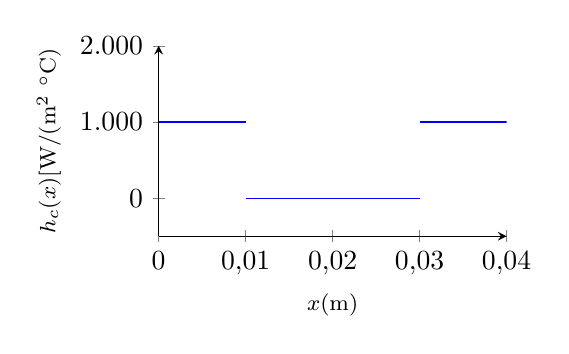
\begin{tikzpicture}
		\begin{axis}[
		/pgf/number format/1000 sep={.},/pgf/number format/use comma,
		axis lines=left,
		xmin = 0,
		xmax = 0.04,
		ymin = -500,
		ymax = 2000,
		restrict y to domain=-500:2000,
		scaled x ticks = false,
		scaled y ticks = false,
		x tick label style={/pgf/number format/fixed},
		y tick label style={/pgf/number format/fixed},
		anchor=east,  
		width=6cm,
		height=4cm,
		label style={font=\footnotesize},
		xlabel = $x$(m),
		ylabel= $h_c(x)[$W/($\text{m}^2$ \celsius)]]
		\addplot[color=blue,mark=none,smooth, domain=0:0.01] {1000};
		\addplot[color=blue,mark=none,smooth, domain=0.01:0.03] {0};
		\addplot[color=blue,mark=none,smooth, domain=0.03:0.04] {1000};
		\end{axis}
		\end{tikzpicture}
		\caption*{(a) Perfil 1}
	\end{minipage}
\end{figure}
%	\begin{minipage}[t][5cm][t]{0,5\textwidth}
%		\begin{tikzpicture}
%		\begin{axis}[
%		axis lines=left,
%		xmin = 0,
%		xmax = 0.04,
%		ymin = -500,
%		ymax = 2000,
%		restrict y to domain=-500:2000,
%		scaled x ticks = false,
%		scaled y ticks = false,
%		x tick label style={/pgf/number format/fixed},
%		y tick label style={/pgf/number format/fixed},
%		anchor=east,  
%		width=6cm,
%		height=4cm,
%		label style={font=\footnotesize},
%		xlabel = $x$(m),
%		ylabel= $h_c(x)$[W/($\text{m}^2$ \celsius)]]
%		\pgfplotstableread{../data/conductance_02.dat} 
%		\teff
%		\addplot[color=blue,mark=none,smooth] table from \teff;
%		\end{axis}
%		\end{tikzpicture}
%		\caption*{(a) Perfil 2}
%	\end{minipage}
\begin{figure}[h!b]
	\begin{minipage}[t][5cm][c]{\textwidth}
		\centering
		\begin{tikzpicture}
		\begin{axis}[
		/pgf/number format/1000 sep={.},/pgf/number format/use comma,
		axis lines=left,
		xmin = 0,
		xmax = 0.04,
		ymin = -500,
		ymax = 2000,
		restrict y to domain=-500:2000,
		scaled x ticks = false,
		scaled y ticks = false,
		x tick label style={/pgf/number format/fixed},
		y tick label style={/pgf/number format/fixed},
		anchor=east,  
		width=6cm,
		height=4cm,
		label style={font=\footnotesize},
		xlabel = $x$(m),
		ylabel= $h_c(x)$[W/($\text{m}^2$ \celsius)]]
		\pgfplotstableread{../data/conductance_02.dat} 
		\teff
		\addplot[color=blue,mark=none,smooth] table from \teff;
		\end{axis}
		\end{tikzpicture}
		\caption*{(a) Perfil 2}
	\end{minipage}
\end{figure}
\newpage
%	\begin{minipage}[t][5cm][t]{0,5\textwidth}
%		\begin{tikzpicture}
%		\begin{axis}[
%		axis lines=left,
%		xmin = 0,
%		xmax = 0.04,
%		ymin = -500,
%		ymax = 2000,
%		restrict y to domain=-500:2000,
%		scaled x ticks = false,
%		scaled y ticks = false,
%		x tick label style={/pgf/number format/fixed},
%		y tick label style={/pgf/number format/fixed},
%		anchor=east,  
%		width=6cm,
%		height=4cm,
%		label style={font=\footnotesize},
%		xlabel = $x$(m),
%		ylabel= $h_c(x)$[W/($\text{m}^2$ \celsius)]]
%		\pgfplotstableread{../data/conductance_04.dat} 
%		\teff
%		\addplot[color=blue,mark=none,smooth] table from \teff;
%		\end{axis}
%		\end{tikzpicture}
%		\caption*{(a) Perfil 4}
%	\end{minipage}
%	\begin{minipage}[t][5cm][t]{0,5\textwidth}
%		\begin{tikzpicture}
%		\begin{axis}[
%		axis lines=left,
%		xmin = 0,
%		xmax = 0.04,
%		ymin = -500,
%		ymax = 2000,
%		restrict y to domain=-500:2000,
%		scaled x ticks = false,
%		scaled y ticks = false,
%		x tick label style={/pgf/number format/fixed},
%		y tick label style={/pgf/number format/fixed},
%		anchor=east,  
%		width=6cm,
%		height=4cm,
%		label style={font=\footnotesize},
%		xlabel = $x$(m),
%		ylabel= $h_c(x)$[W/($\text{m}^2$ \celsius)]]
%		\pgfplotstableread{../data/conductance_05.dat} 
%		\teff
%		\addplot[color=blue,mark=none,smooth] table from \teff;
%		\end{axis}
%		\end{tikzpicture}
%		\caption*{(a) Perfil 5}
%	\end{minipage}
\begin{figure}[h!b]
	\begin{minipage}[t][5cm][c]{\textwidth}
		\centering
		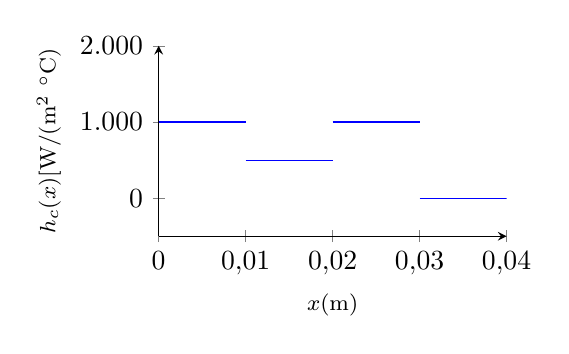
\begin{tikzpicture}
		\begin{axis}[
		/pgf/number format/1000 sep={.},/pgf/number format/use comma,
		axis lines=left,
		xmin = 0,
		xmax = 0.04,
		ymin = -500,
		ymax = 2000,
		restrict y to domain=-500:2000,
		scaled x ticks = false,
		scaled y ticks = false,
		x tick label style={/pgf/number format/fixed},
		y tick label style={/pgf/number format/fixed},
		anchor=east,  
		width=6cm,
		height=4cm,
		label style={font=\footnotesize},
		xlabel = $x$(m),
		ylabel= $h_c(x)$[W/($\text{m}^2$ \celsius)]]
		\addplot[color=blue,mark=none,smooth, domain=0:0.01] {1000};
		\addplot[color=blue,mark=none,smooth, domain=0.01:0.02] {500};
		\addplot[color=blue,mark=none,smooth, domain=0.02:0.03] {1000};
		\addplot[color=blue,mark=none,smooth, domain=0.03:0.04] {0};
		\end{axis}
		\end{tikzpicture}
		\caption*{(a) Perfil 3}
	\end{minipage}	
	\caption{Diferentes perfis de $h_c(x)$ na interface $\Gamma$}
	\label{figura_ctc}
\end{figure}


\subsection{Determinação das temperaturas sintéticas}

As medidas de temperatura na superfície superior $\Gamma_0$ do corpo de prova, representadas por $Y$ nas expressões \eqref{calculo_FR_F1_antes} e \eqref{calculo_FR_G1_antes}, foram obtidas resolvendo o problema direto definido na seção \ref{sec_formulacao_direta}, com os parâmetros, perfis de CTC e geometrias de interface indicados nas seções \ref{config_fis_geom} e \ref{config_ctc}. A fim de evitar a ocorrência do ``crime inverso", isto é, uma redução artificial do mal condicionamento do problema inverso quando o método empregado para resolvê-lo é o mesmo aplicado ao problema direto que fornece as medidas sintéticas\citep{livro_kaipio}, foram executadas simulações das diferentes configurações do problema direto no COMSOL \textit{Multiphysics}\textsuperscript{\textregistered}. O COMSOL é um \textit{software} comercial de elementos finitos, que possui um módulo específico para simulações de transferência de calor.

As várias configurações possíveis do problema direto definido na seção \ref{sec_formulacao_direta} foram modeladas e simuladas neste programa, seguindo os dados apresentados nas tabelas \ref{tabela_params}, \ref{tabela_interfaces} e \ref{tabela_ctc}, usando uma malha triangular extrafina. Para cada configuração, os valores de temperatura ao longo da interface superior $\Gamma_0$ foram exportados em arquivos-texto e usados como entrada para o programa implementado para a estimativa da CTC, e que será comentado na seção \ref{sobre_o_programa}. Convencionou-se extrair um total de 121 pontos equidistantes de medição de temperatura sobre a superfície $\Gamma_0$ para cada configuração.

Para fins de verificação, as mesmas combinações foram resolvidas numericamente através do método da Transformada Integral Clássica, e os resultados obtidos para a distribuição de temperaturas sobre a superfície $\Gamma_0$ apresentaram boa aderência com os obtidos a partir do COMSOL. A título de exemplo, as figuras \ref{fig_comparativo_1} e \ref{fig_comparativo_2} apresentam, respectivamente, um comparativo entre as temperaturas levantadas na superfície superior do corpo de prova, para a configuração específica referente à interface 3 e condutância de contato 2, e a distribuição do desvio relativo percentual entre essas medidas, calculada por:
\begin{align}
\epsilon_i = 100\abs{\frac{T\textsuperscript{COMSOL}_i - T\textsuperscript{CITT}_i}{T\textsuperscript{COMSOL}_i}}, i \in \Gamma_0
\end{align}

\begin{figure}[H]
	\begin{minipage}[t][8cm][c]{\textwidth}
		\centering
		\begin{tikzpicture}
		\begin{axis}[
		/pgf/number format/1000 sep={.},/pgf/number format/use comma,
		axis lines=left,
		%		xmin = 0,
		%		xmax = 0.04,
		%		ymin = 310,
		%		ymax = 340,
		%		restrict y to domain=-500:2000,
		scaled x ticks = false,
		scaled y ticks = false,
		x tick label style={/pgf/number format/fixed},
		y tick label style={/pgf/number format/fixed},
		anchor=east,  
		width=7cm,
		height=5cm,
		label style={font=\footnotesize},
		xlabel = $x$(m),
		ylabel= $T_1\big|_{\Gamma_0}$ (\celsius)]
		\pgfplotstableread{../data/fortran/temperaturas_sinteticas_interface_03_conductance_03.dat} 
		\teff
		\addplot[color=blue,mark=o,mark options={mark size=1.0pt}] table from \teff;
		\pgfplotstableread{../data/comsol/temperaturas_sinteticas_interface_03_conductance_03.dat} 
		\teff
		\addplot[only marks,color=red,mark=square,mark options={mark size=1.0pt}] table from \teff;
		\end{axis}
		\end{tikzpicture}
		\caption{Temperatura na superfície superior $\Gamma_0$ para a configuração referente à interface 3 e condutância de contato 3: $\textcolor{blue}{\ocircle} \rightarrow$ CITT; $\textcolor{red}{\square} \rightarrow$ Elementos finitos (COMSOL)}
		\label{fig_comparativo_1}
	\end{minipage}
	\begin{minipage}[t][8cm][c]{\textwidth}
		\centering
		\begin{tikzpicture}
		\begin{axis}[
		/pgf/number format/1000 sep={.},/pgf/number format/use comma,
		axis lines=left,
		%		xmin = 0,
		%		xmax = 0.04,
		%		ymin = 0.085,
		%		ymax = 0.105,
		%		restrict y to domain=-500:2000,
		scaled x ticks = false,
		scaled y ticks = false,
		x tick label style={/pgf/number format/fixed},
		y tick label style={/pgf/number format/fixed, /pgf/number format/precision=5},
		anchor=east,  
		width=7cm,
		height=5cm,
		label style={font=\footnotesize},
		xlabel = $x$(m),
		ylabel= $\epsilon$ (\%)]
		\pgfplotstableread{../data/desvio_relativo_interface_03_conductance_03.dat} 
		\teff
		\addplot[mark=o,mark options={mark size=1.0pt}] table from \teff;
		\end{axis}
		\end{tikzpicture}
		\caption{Desvio percentual entre as temperaturas obtidas via CITT e método dos elementos finitos (COMSOL), na superfície superior $\Gamma_0$ para a configuração referente à interface 3 e condutância de contato 3}
		\label{fig_comparativo_2}
	\end{minipage}
\end{figure}

As temperaturas sintéticas obtidas a partir do COMSOL correspondem a medidas consideradas exatas, sem ruídos ou erros experimentais. De forma a simular medidas com erros experimentais, foi implementado o mesmo procedimento adotado por \cite{tese_padilha}: foram adicionados erros randômicos com distribuição normal às temperaturas calculadas sobre a superfície superior do corpo de prova. Sendo então $\mathbf{Y}$ as medidas de temperatura simuladas sem erros, as medidas simuladas com erros, denotadas por $\tilde{\mathbf{Y}}$, foram calculadas através da expressão:
\begin{align}
\tilde{\mathbf{Y}} = \mathbf{Y} + \mathbf{\varepsilon} \sigma \label{modelagem_erro}
\end{align}
onde $\sigma$ é o desvio padrão das medidas de temperatura, e $\varepsilon$ é uma sequência aleatória gerada a partir da transformação Box-Muller\citep{artigo_box_muller}:
\begin{align}
\varepsilon = \cos(2\pi v)\sqrt{-2 \ln u}
\end{align}
onde $u$ e $v$ correspondem a variáveis aleatórias contínuas com distribuição uniforme entre 0 e 1.

Três níveis de desvio-padrão foram testados: $\sigma = \text{0,0}\celsius$ (correspondente aos casos onde as temperaturas sintéticas não contém erros), $\sigma = \text{0,1}\celsius$ e $\sigma = \text{0,5}\celsius$. Desse modo, havendo três possibilidades de geometrias de interface de contato e três possibilidades de condutância térmica de contato teórica, foram realizadas nove simulações distintas de problemas-teste diretos, para obtenção das respectivas distribuições de temperaturas sintéticas exatas. A cada um desses resultados foram aplicados os erros correpondentes às três possibilidades de desvio-padrão, num total de 27 conjuntos de dados de entrada; estes dados por sua vez alimentaram cada um dos 27 problemas inversos equivalentes resolvidos neste trabalho. Nas figuras \ref{figura_temperaturas_sinteticas_interface_01}, \ref{figura_temperaturas_sinteticas_interface_02} e \ref{figura_temperaturas_sinteticas_interface_03}, é possível visualizar as distribuições de temperaturas sintéticas na superfície superior do corpo de prova para cada uma das configurações. A maior ou menor dispersão dos dados com erros aleatórios em torno das medidas exatas é devida apenas às diferentes escalas adotadas no eixo $y$ de cada gráfico.

\begin{figure}[H]
	\graficostemperatura{1}{1}{a}{310}{345}
	\graficostemperatura{1}{2}{b}{251}{277}
	\graficostemperatura{1}{3}{c}{260}{330}
	\caption{Temperaturas sintéticas ($Y$) ao longo da superfície superior $\Gamma_0$, para os perfis de CTC de 1 a 3, referentes à interface de contato 1: $\textcolor{blue}{\ocircle} \rightarrow \sigma = 0,0$; $\textcolor{red}{\square} \rightarrow \sigma = 0,1$; $\textcolor{gray}{\triangle} \rightarrow \sigma = 0,5$}
	\label{figura_temperaturas_sinteticas_interface_01}
\end{figure}
\begin{figure}[H]
	\graficostemperatura{2}{1}{a}{310}{345}
	\graficostemperatura{2}{2}{b}{251}{277}
	\graficostemperatura{2}{3}{c}{260}{330}
	\caption{Temperaturas sintéticas ($Y$) ao longo da superfície superior $\Gamma_0$, para os perfis de CTC de 1 a 3, referentes à interface de contato 2: $\textcolor{blue}{\ocircle} \rightarrow \sigma = 0,0$; $\textcolor{red}{\square} \rightarrow \sigma = 0,1$; $\textcolor{gray}{\triangle} \rightarrow \sigma = 0,5$}
	\label{figura_temperaturas_sinteticas_interface_02}
\end{figure}
\begin{figure}[H]
	\graficostemperatura{3}{1}{a}{310}{345}
	\graficostemperatura{3}{2}{b}{251}{277}
	\graficostemperatura{3}{3}{c}{260}{330}
	\caption{Temperaturas sintéticas ($Y$) ao longo da superfície superior $\Gamma_0$, para os perfis de CTC de 1 a 3, referentes à interface de contato 3: $\textcolor{blue}{\ocircle} \rightarrow \sigma = 0,0$; $\textcolor{red}{\square} \rightarrow \sigma = 0,1$; $\textcolor{gray}{\triangle} \rightarrow \sigma = 0,5$}
	\label{figura_temperaturas_sinteticas_interface_03}
\end{figure}

\subsection{Interpolação das temperaturas sintéticas}\label{secao_interpolacao}
Sejam as expressões dos funcionais de reciprocidade associados às funções auxiliares $F_{1, j}$ e $G_{1, j}$, deduzidas no capítulo anterior:
\begin{align}
\Re(F_{1,j})
& =
-\frac{q}{k_1}\bar{\psi}_{j,0} + \frac{\mathbb{A}_{j,0} - \bar{\psi}_{j,0}}{ab}\int_0^a Y(x)dx + \nonumber \\
& \frac{2}{a}\sum_{m=1}^M \mu_m \left(\frac{\mathbb{A}_{j,m}}{\sinh\mu_m b} - \frac{\bar{\psi}_{j, m}}{\tanh\mu_m b}\right)\int_0^a Y(x)\cos\mu_m x dx
\label{calculo_FR_F1_antes_a} \\ \nonumber \\
\Re(G_{1,j})
& =
-\frac{q}{k_1}\bar{\phi}_{j,0} + \frac{\mathbb{E}_{j,0} - \bar{\phi}_{j,0}}{ab}\int_0^a Y(x)dx + \nonumber \\
& \frac{2}{a}\sum_{m=1}^M \mu_m \left(\frac{\mathbb{E}_{j,m}}{\sinh\mu_m b} - \frac{\bar{\phi}_{j, m}}{\tanh\mu_m b}\right)\int_0^a Y(x)\cos\mu_m x dx
\label{calculo_FR_G1_antes_a}
\end{align}

Foi comentado anteriormente que a função $Y(x)$ representa as medidas experimentais de temperatura na superfície superior do corpo de prova, obtidas artificialmente neste trabalho, através de simulação do problema direto. As integrais acima poderiam então ser imediatamente identificadas com a transformação integral da função $Y(x)$.

Na prática, porém, a função $Y(x)$ é desconhecida, e dispõe-se apenas de dados discretos, correspondentes às temperaturas medidas em pontos distintos da superfície superior. No trabalho de \cite{tese_padilha}, foi feita uma aproximação dessa função $Y(x)$ através de uma \textit{spline} que interpolava essas medidas. Uma outra forma de interpolar as medidas sintéticas, por meio de uma expansão em série de funções ortogonais às autofunções do problema de autovalor, foi proposta por \cite{artigo_mocerino} em seu trabalho de determinação de coeficiente de troca térmica de calor na parte interna de tubulações de trocadores de calor, que também empregou a técnica dos funcionais de reciprocidade. Desse modo, aplicando a segunda abordagem no caso em estudo, a função $Y(x)$ poderia ser escrita na forma
\begin{align}
Y(x) \approx \bar{y}_0 + \sum_{m=1}^M \bar{y}_m \cos\mu_m x \label{aproximacao_Y}
\end{align}

Não é difícil observar que a expressão acima é, basicamente, o truncamento da expansão de $Y(x)$ em somatório infinito de autofunções. Assim, podem-se estabelecer as seguintes relações entre os coeficientes $\bar{y}_m, m=0,1,2,...,M$ e as transformadas integrais de $Y(x)$:
\begin{align}
& \bar{y}_0 = \frac{1}{a}\int_0^a Y(x) dx \\ \nonumber \\
& \bar{y}_m = \frac{2}{a}\int_0^a Y(x) \cos\mu_m x dx, \qquad m = 1, 2, ..., M
\end{align}

Substituindo em \eqref{calculo_FR_F1_antes_a} e \eqref{calculo_FR_G1_antes_a}, obtém-se:
\begin{align}
\Re(F_{1,j})
& =
-\frac{q}{k_1}\bar{\psi}_{j,0} + \frac{\mathbb{A}_{j,0} - \bar{\psi}_{j,0}}{b} \bar{y}_0 + \sum_{m=1}^M \mu_m \left(\frac{\mathbb{A}_{j,m}}{\sinh\mu_m b} - \frac{\bar{\psi}_{j, m}}{\tanh\mu_m b}\right)\bar{y}_m
\label{calculo_FR_F1_antes_b} \\ \nonumber \\
\Re(G_{1,j})
& =
-\frac{q}{k_1}\bar{\phi}_{j,0} + \frac{\mathbb{E}_{j,0} - \bar{\phi}_{j,0}}{b} \bar{y}_0 + \sum_{m=1}^M \mu_m \left(\frac{\mathbb{E}_{j,m}}{\sinh\mu_m b} - \frac{\bar{\phi}_{j, m}}{\tanh\mu_m b}\right)\bar{y}_m
\label{calculo_FR_G1_antes_b}
\end{align}

Desse modo, as expressões \eqref{calculo_FR_F1_antes_b} e \eqref{calculo_FR_G1_antes_b} permitem determinar os funcionais de reciprocidade $\Re(F_{1,j})$ e $\Re(G_{1,j})$, apenas conhecendo os coeficientes $\bar{y}_0, \bar{y}_1, \bar{y}_2, ..., \bar{y}_M$ da aproximação \eqref{aproximacao_Y}. Estes coeficientes, por sua vez, podem ser calculados através da solução de aproximação por mínimos quadrados do problema, formulada a partir da aproximação sugerida em \eqref{aproximacao_Y}:
\begin{align}
\begin{bmatrix}
Y_0 \\ Y_1 \\ Y_2 \\ \vdots \\ Y_{imax}
\end{bmatrix}
=
\begin{bmatrix}
1 & \cos\mu_1 x_0 & \cos \mu_2 x_0 & ... & \cos\mu_M x_0 \\
1 & \cos\mu_1 x_1 & \cos \mu_2 x_1 & ... & \cos\mu_M x_1 \\
1 & \cos\mu_1 x_2 & \cos \mu_2 x_2 & ... & \cos\mu_M x_2 \\
... & ... & ... & \ddots & ... \\
1 & \cos\mu_1 x_{imax} & \cos \mu_2 x_{imax} & ... & \cos\mu_M x_{imax}
\end{bmatrix}
\times
\begin{bmatrix}
\bar{y}_0 \\ \bar{y}_1 \\ \bar{y}_2 \\ \vdots \\ \bar{y}_M
\end{bmatrix}
\label{sistema_aproximacao_Y}
\end{align}
onde cada par $(x_i, Y_i)$ corresponde respectivamente a um abscissa sobre a superfície superior do corpo de prova e o valor medido de temperatura naquele ponto.


\subsection{Definição das funções $\psi_j(x)$ e $\phi_j(x)$}
Uma questão que ficou em aberto até o momento é a que envolve a definição das funções $\psi_j(x)$ e $\phi_j(x)$, necessárias para a determinação das funções $\beta_j(x)$ e $\gamma_j(x)$. Neste trabalho foram empregadas as seguintes alternativas para estas funções:
\begin{align}
\psi_j(x), \phi_j(x) = \left\lbrace
\begin{array}{ll}
\displaystyle\sqrt{\frac{1}{a}}, & j = 0 \\ \nonumber \\
\displaystyle\sqrt{\frac{2}{a}}\cos \mu_j x, & j = 1,2,3,\ldots
\end{array}
\right.
\end{align} 

Estas funções foram as mesmas usadas por \cite{tese_padilha} na sua tese de doutorado e se mostraram bastante vantajosas do ponto de vista computacional, tanto neste como naquele trabalho. De fato, no estudo do problema de determinação da CTC numa interface plana horizontal no referido trabalho, foi demonstrado que o emprego destas funções diretamente nas condições de contorno dos problemas auxiliares para $F_{1,j}$, $F_{2,j}$ e $G_{1,j}$ garantia automaticamente a ortogonalidade das funções $\beta_j(x)$ e $\gamma_j(x)$. Já no presente trabalho, o grande benefício no uso destas funções reside na simplificação do cálculo das respectivas transformadas integrais:
\begin{align}
\bar{\psi}_{j, m}, \bar{\phi}_{j, m} = \left\lbrace
\begin{array}{ll}
\displaystyle\sqrt{\frac{a}{2}}, & j = m \ne 0 \\ \nonumber \\
\displaystyle\sqrt{a}, & j = m = 0 \\ \nonumber \\
0, & j \ne m 
\end{array}
\right.
\end{align}

\subsection{Código computacional}\label{sobre_o_programa}

Neste trabalho, o código computacional foi desenvolvido usando a linguagem de programação Fortran 2003. O compilador usado foi o \textit{gfortran}, que faz parte do projeto de \textit{software} livre GCC. O ambiente de desenvolvimento, onde o código era editado, compilado e depurado, foi o Eclipse, que também é um \textit{software} não-comercial. Todo o trabalho foi desenvolvido num computador executando o sistema operacional Linux para plataforma de 64 bits; no caso, a distribuição do sistema operacional usada foi Ubuntu versão 16.04.

As rotinas numéricas empregadas foram obtidas do projeto Netlib\footnote{Mais informações sobre o repositório Netlib podem ser encontradas no endereço de Internet \href{https://www.netlib.org/}{https://www.netlib.org/}.}, que é um repositório \textit{online} mantido por algumas instituições e universidades, contendo \textit{software} de computação científica e documentação disponíveis gratuitamente. A maioria das rotinas encontradas no repositório Netlib está escrita em FORTRAN 77\footnote{O uso de caixa alta para designar a versão 77 da linguagem Fortran tem raízes históricas, sendo encontrado em muitas publicações, e por isso esta convenção foi mantida aqui.}, especialmente as usadas no programa desenvolvido para este trabalho, o que não trouxe dificuldades, pois o compilador \textit{gfortran} é capaz de efetuar a compilação híbrida de arquivos-fonte escritos tanto em FORTRAN 77 quanto em Fortran 2003, inclusive padronizando para que todas as variáveis de ponto flutuante de precisão simples sejam tratadas como sendo de precisão dupla, o que de fato foi feito no programa.
A livre disponibilidade do código-fonte das rotinas facilitou significativamente a depuração do programa e a consequente identificação e correção de erros, sendo um fator determinante no desenvolvimento do mesmo. 

Foram empregadas rotinas numéricas do repositório Netlib para realizar as seguintes tarefas:
\begin{itemize}
	\item Cálculo dos coeficientes $\bar{y}_0, \bar{y}_1, \bar{y}_2, ..., \bar{y}_M$ presentes nas equações \eqref{calculo_FR_F1_antes_b} e \eqref{calculo_FR_G1_antes_b}, calculados a partir da solução de mínimos quadrados do sistema \eqref{sistema_aproximacao_Y}. O repositório Netlib possui o subprojeto LAPACK (\textit{Linear Algebra PACKage}), contendo diversos \textit{solvers} de sistemas lineares para várias possibilidades de matrizes de coeficientes: matrizes-banda, simétricas, positivas definidas, etc, além de outros utilitários de Álgebra Linear. Foi utilizada a rotina DGELS, que recebe a matriz e o vetor correspondentes ao sistema, e retorna a solução de mínimos quadrados, além de outras informações, tais como a norma dos resíduos.
%	\item Cálculo das integrais presentes nas equações \eqref{calculo_FR_F1_antes} e \eqref{calculo_FR_G1_antes}. Estas integrais são da forma
%	\begin{align}
%	& \int_0^a Y(x)dx \\ \nonumber \\
%	& \int_0^a Y(x)\cos\mu_m x dx
%	\end{align}
%	Estas integrais devem ser resolvidas numericamente, uma vez que o termo $Y(x)$, referente às temperaturas sintéticas sobre a superfície superior do corpo de prova, corresponde na verdade a um conjunto de dados discretos cuja formulação analítica é desconhecida (num problema real). Foram utilizadas duas rotinas que trabalhavam em conjunto: CURFIT, que aproxima um conjunto de pontos $(x_i, y_i)$ em uma B-\textit{spline}, e SPLINT, que integra a B-\textit{spline} obtida da rotina anterior sobre um intervalo.
	
	\item Cálculo das transformadas integrais que fornecem os coeficientes dos sistemas lineares \eqref{sistema_para_coeficientes_3} e \eqref{sistema_para_coeficientes_21}. O repositório Netlib oferece a rotina DQAWO, que faz parte do subprojeto QUADPACK, e que resolve integrais da forma
	\begin{align}
	& \int_{x_0}^{x_1} f(x)\cos\omega x dx \label{dqawo} \\ \nonumber \\
	& \int_{x_0}^{x_1} f(x)\sin\omega x dx 
	\end{align}
	A rotina foi parametrizada para resolver integrais conforme a expressão \eqref{dqawo}, fazendo $\omega = \mu_m$.
	
	\item Solução numérica dos sistemas de equações lineares \eqref{sistema_para_coeficientes_3} e \eqref{sistema_para_coeficientes_21}. Foi utilizada no trabalho a rotina DGESVX, do subprojeto LAPACK, que recebe como entrada a matriz de coeficientes e uma matriz cujas colunas são diferentes vetores de termos independentes do sistema; a rotina aplica um pré-condicionador ao sistema, realiza uma decomposição LU da matriz de coeficientes e usa este resultado para obter os vetores-solução referentes a cada vetor de termos independentes. Esta rotina atendeu à necessidade de se resolver de forma eficiente um dado sistema de equações, variando apenas o segundo membro correspondente aos termos independentes, o que foi comentado na seção \ref{orto_beta_gama}.
	
	\item Cálculo das integrais necessárias para a ortogonalização de Gram-Schmidt. Estas integrais, definidas de forma geral pela equação \eqref{integral_da_definicao_produto_interno_4}, foram calculadas através da rotina de integração de propósito geral DAQG, que realiza uma integração adaptativa através das fórmulas de quadratura de Gauss-Konrod.
\end{itemize}

Diversas otimizações foram implementadas a fim de minimizar o tempo de processamento, como por exemplo operações diretas com segmentos de matrizes e vetores ao invés de laços iterativos. Tais otimizações levaram a uma melhoria considerável no desempenho do programa como um todo, em especial na fase de ortonormalização de Gram-Schmidt, onde se observava o maior gargalo de processamento. Desse modo, o tempo de execução do código computacional no cálculo de um determinado perfil de condutância térmica de contato não excedia o intervalo de tempo de 2,5 segundos\footnote{Nas execuções realizadas num computador Lenovo Ideapad 330, com processador Intel Core\textsuperscript{\texttrademark} i5-8250U, CPU 1,60 GHz e memória RAM de 8 GB, o tempo total para o levantamento de uma estimativa de perfil de condutância térmica de contato variava entre 2,0 segundos a 2,4 segundos.}.

\subsection{Resultados e análises}

Serão apresentados agora os resultados numéricos obtidos a partir da aplicação das equações \eqref{calculo_FR_F1_antes}, \eqref{calculo_FR_G1_antes} e \eqref{expressao_final_ctc} ao problema inverso de condução de calor descrito no capítulo \ref{sec_prob_inv}. Estas equações fornecem, respectivamente, as estimativas de salto de temperatura, fluxo de calor e condutância térmica de contato na interface entre os materiais que compõem o arranjo físico ilustrado na figura \ref{fig2}.

Para cada combinação possível de geometria de interface (Tabela \ref{tabela_interfaces}), perfil de condutância térmica de contato (Tabela \ref{tabela_ctc}) e desvio-padrão de erros de medição ($\sigma = \text{0,0}\celsius$, $\sigma = \text{0,1}\celsius$ e $\sigma = \text{0,5}\celsius$), foram calculadas estimativas de salto de temperatura e fluxo de calor na interface de contato, e os resultados foram comparados com os respectivos valores teóricos esperados para cada combinação. A estimativa do perfil de condutância térmica de contato, calculada através da razão entre o fluxo de calor e o salto de temperatura estimados na interface, também foi comparada com o perfil teórico correspondente, e que foi usado para determinação prévia das temperaturas sintéticas através de simulações de cada configuração do problema no módulo de transferência de calor no simulador COMSOL \textit{Multiphysics}\textsuperscript{\textregistered}.

Não foi realizada uma análise de convergência rigorosa dos somatórios nas expressões \eqref{serie_para_beta}, \eqref{serie_para_gamma}, \eqref{calculo_FR_F1_antes_b} e \eqref{calculo_FR_G1_antes_b}, que fornecem as funções $\beta_j$ e $\gamma_j$ e os funcionais de reciprocidade $\Re(F_{1,j})$ e $\Re(G_{1,j})$. Adotou-se $M=20$ para o número de autofunções empregados nos somatórios que fornecem $\beta_j$, $\gamma_j$ e para o número de termos a serem somados para determinação dos funcionais de reciprocidade.

Os limites superiores $N_1$ e $N_2$, dos somatórios que fornecem o cálculo do salto de temperatura -- eq. \eqref{resultado_1} -- e do fluxo de calor -- eq. \eqref{resultado_2} -- na interface de contato, não foram os mesmos para todos os casos analisados, sendo estabelecidos os seguintes limites máximos:
\begin{itemize}
	\item $N_1 \le 20$ (número máximo de funcionais de reciprocidade calculados para as expansões de salto de temperatura)
	\item $N_2 \le 20$ (número máximo de funcionais de reciprocidade calculados para as expansões de fluxo de calor)
\end{itemize}

Posteriormente serão tecidos comentários quanto ao caráter instável dos somatórios referentes aos cálculos do salto de temperatura e do fluxo de calor, bem quanto às dificuldades de estabelecimento de critérios de parada destes somatórios.

Os gráficos utilizados na análise estão agrupados por geometria de interface; em cada grupo, estão plotadas as estimativas de salto de temperatura e fluxo de calor na interface de contato. A estimativa da condutância térmica de contato é representada no último subgrupo de gráficos para cada interface. A fim de auxiliar na verificação da qualidade das estimativas, também é apresentada uma tabela correspondente para cada subgrupo de gráficos, contendo os valores de desvio quadrático médio das estimativas em relação ao resultado teórico esperado para a variável associada.

\subsubsection{Estimativas para a geometria de interface de contato 1}

A primeira geometria de interface de contato para a qual foram realizadas estimativas de condutância térmica de contato é a referente ao índice 1 na tabela \ref{tabela_interfaces}. Esse formato de interface, basicamente uma superfície plana e horizontal paralela às bases do corpo de prova de seção reta retangular (cf. Figura \ref{figura_interfaces}), corresponde exatamente à configuração inicialmente estudada por \cite{reciproc_3}, e que culminou no trabalho desenvolvido por \cite{tese_padilha}. Esta configuração foi o ponto de partida das primeiras pesquisas envolvendo a aplicação do método dos Funcionais de Reciprocidade na estimativa da condutância térmica de contato. Desse modo, este problema-teste serviu como base de referência para verificação da metodologia proposta neste trabalho.

As estimativas para o salto de temperatura ao longo da interface de contato, correspondentes aos três perfis teóricos de CTC, estão plotadas nos gráficos da Figura \ref{figura_delta_temperaturas_interface_01}. 
\begin{figure}[H]
	\graficoestimativa{delta_temperatura}{1}{1}{20}{06}{02}{a}{\Delta T\big|_{\Gamma}}{\celsius}
	\graficoestimativa{delta_temperatura}{1}{2}{20}{04}{02}{b}{\Delta T\big|_{\Gamma}}{\celsius}
	\graficoestimativa{delta_temperatura}{1}{3}{20}{06}{03}{c}{\Delta T\big|_{\Gamma}}{\celsius}
	\caption{Comparação entre as estimativas de $[T_1 - T_2]_\Gamma$ e os valores exatos para os perfis de CTC de 1 a 3, referentes à interface de contato 1: $\text{--} \rightarrow \text{Exato}$; $\textcolor{blue}{\ocircle} \rightarrow \sigma = 0,0$; $\textcolor{red}{\square} \rightarrow \sigma = 0,1$; $\textcolor{gray}{\triangle} \rightarrow \sigma = 0,5$}
	\label{figura_delta_temperaturas_interface_01}
\end{figure}

A Tabela \ref{tabela_rms_delta_temperaturas_interface_1} mostra os valores de desvio quadrático médio entre as medidas estimadas e as teóricas de salto de temperatura para cada perfil teórico de condutância térmica de contato. É possível notar, por inspeção dos valores na tabela, como as estimativas calculadas para $\sigma = \text{0,0}\celsius$ são consideravelmente melhores.
\begin{table}[H]
	\centering
	\caption{Desvio quadrático médio das estimativas de salto de temperatura para a interface de contato 1}
	\begin{tabular}{c|c|c|c|}
		\cline{2-4}
		& \multicolumn{3}{c|}{$\text{RMS}_{\Delta T} (\celsius)$} \\ \hline
		\multicolumn{1}{|c|}{Perfil} & $\sigma = \text{0,0}\celsius$   & $\sigma = \text{0,1}\celsius$    & $\sigma = \text{0,5}\celsius$  \\ \hline
		\multicolumn{1}{|c|}{1}      &  0,0490      & 0,3222       & 0,5441       \\ \hline
		\multicolumn{1}{|c|}{2}      &  0,0024      & 0,1320       & 0,3437      \\ \hline
		\multicolumn{1}{|c|}{3}      &  0,0350      & 0,2980       & 0,6154      \\ \hline
	\end{tabular}
	\label{tabela_rms_delta_temperaturas_interface_1}
\end{table}

Verificou-se uma excelente concordância entre as estimativas e os valores exatos; para o caso específico em que o desvio padrão é zero, as estimativas praticamente coincidiram com as medidas sintéticas. Notou-se também que as regiões em que o salto de temperatura atinge valores maiores correspondem às regiões onde a condutância térmica é menor. Assim, o comportamento da distribuição estimada do salto de temperatura mostrou-se consistente com o comportamento teórico esperado.

As estimativas para o fluxo de calor ao longo da interface de contato, correspondentes aos três perfis teóricos de CTC, estão plotadas nos gráficos da Figura \ref{figura_fluxo_calor_interface_01}.  
\begin{figure}[H]
	\graficoestimativa{fluxo_calor}{1}{1}{20}{06}{02}{a}{-k_1 \frac{\partial T_1}{\partial\mathbf{n}_1}\big|_{\Gamma}}{W/$\text{m}^2$}
	\graficoestimativa{fluxo_calor}{1}{2}{20}{04}{02}{b}{-k_1 \frac{\partial T_1}{\partial\mathbf{n}_1}\big|_{\Gamma}}{W/$\text{m}^2$}
	\graficoestimativa{fluxo_calor}{1}{3}{20}{06}{03}{c}{-k_1 \frac{\partial T_1}{\partial\mathbf{n}_1}\big|_{\Gamma}}{W/$\text{m}^2$}
	\caption{Comparação entre as estimativas de $[-k_1 {\partial T_1}/{\partial\mathbf{n}_1}]_\Gamma$ e os valores exatos para os perfis de CTC de 1 a 3, referentes à interface de contato 1: $\text{--} \rightarrow \text{Exato}$; $\textcolor{blue}{\ocircle} \rightarrow \sigma = 0,0$; $\textcolor{red}{\square} \rightarrow \sigma = 0,1$; $\textcolor{gray}{\triangle} \rightarrow \sigma = 0,5$}
	\label{figura_fluxo_calor_interface_01}
\end{figure}

A Tabela \ref{tabela_rms_fluxo_calor_interface_1} mostra os valores de desvio quadrático médio entre as medidas estimadas e as teóricas de fluxo de calor para cada perfil teórico de condutância térmica de contato. Comparando com os valores plotados nos gráficos da Figura \ref{figura_fluxo_calor_interface_01}, pode-se notar que, em termos relativos, os desvios quadráticos médios para $\sigma = \text{0,0}\celsius$ são os que fornecem melhores resultados.
\begin{table}[H]
	\centering
	\caption{Desvio quadrático médio das estimativas de fluxo de calor para a interface de contato 1}
	\begin{tabular}{c|c|c|c|}
		\cline{2-4}
		& \multicolumn{3}{c|}{$\text{RMS}_{q}(\text{W/m}^2)$} \\ \hline
		\multicolumn{1}{|c|}{Perfil} & $\sigma = \text{0,0}\celsius$   & $\sigma = \text{0,1}\celsius$    & $\sigma = \text{0,5}\celsius$  \\ \hline
		\multicolumn{1}{|c|}{1}      & 1268,71        &  2533,25      & 3308,72          \\ \hline
		\multicolumn{1}{|c|}{2}      & 64,68       &  564,06      &  1088,11     \\ \hline
		\multicolumn{1}{|c|}{3}      & 888,39        & 1970,43       & 2691,75        \\ \hline
	\end{tabular}
	\label{tabela_rms_fluxo_calor_interface_1}
\end{table}

Novamente pôde ser observada uma boa coerência entre as estimativas e os valores exatos. No caso $\sigma = \text{0,0}\celsius$ em especial, nota-se a manifestação de um fenômeno semelhante ao efeito Gibbs\citep{livro_boyce} para os perfis de condutância teóricos 1 e 3, que apresentam descontinuidades. O comportamento qualitativo do fluxo de calor também foi consistente com o esperado; de fato, fluxos de calor mais altos correspondiam a regiões em que a condutância térmica era maior.

Uma vez conhecidas as estimativas de fluxo de calor e salto de temperatura na interface de contato, a razão entre essas grandezas em cada ponto $x$ do domínio da interface ($0 \le x \le a$, onde $a$ é o comprimento do corpo de prova) fornece a estimativa do perfil de condutância térmica de contato, conforme a definição apresentada na equação \eqref{eq:definicao_3}. Desse modo, chega-se aos resultados representados graficamente na Figura \ref{figura_ctc_interface_01}\footnote{Os valores negativos de condutância térmica de contato, correspondentes aos perfis 1 e 3, não possuem significado físico, sendo consequência do comportamento oscilatório das funções $\psi_j(x)$ e $\phi_j(x)$ e das descontinuidades nestes perfis.}.
\begin{figure}[H]
	\graficoctc{01}{01}{1}{a}
	\graficoctc{01}{02}{2}{b}
	\graficoctc{01}{03}{3}{c}
	\caption{Comparação entre as estimativas de $h_c$ e os valores exatos para os perfis de CTC de 1 a 3, referentes à interface de contato 1: $\text{--} \rightarrow \text{Exato}$; $\textcolor{blue}{\ocircle} \rightarrow \sigma = 0,0$; $\textcolor{red}{\square} \rightarrow \sigma = 0,1$; $\textcolor{gray}{\triangle} \rightarrow \sigma = 0,5$}
	\label{figura_ctc_interface_01}
\end{figure}

A Tabela \ref{tabela_rms_ctc_interface_1} mostra os valores de desvio quadrático médio entre as medidas estimadas e as teóricas de condutância térmica de contato, para os três perfis analisados. A razão entre cada desvio quadrático médio e o valor máximo da condutância térmica de contato teórica ($h_{max} = 400 \text{ W/m}^2$ \celsius) varia de 0,00495 a 0,22955.
\begin{table}[H]
	\centering
	\caption{Desvio quadrático médio das estimativas de condutância térmica de contato para a interface de contato 1}
	\begin{tabular}{c|c|c|c|}
		\cline{2-4}
		& \multicolumn{3}{c|}{$\text{RMS}_{h_c}(\text{W/m}^{2}$$\celsius)$} \\ \hline
		\multicolumn{1}{|c|}{Perfil} & $\sigma = \text{0,0}\celsius$   & $\sigma = \text{0,1}\celsius$    & $\sigma = \text{0,5}\celsius$  \\ \hline
		\multicolumn{1}{|c|}{1}      & 40,94       & 71,23           & 89,42       \\ \hline
		\multicolumn{1}{|c|}{2}      & 1,98       &  19,66      &   35,42    \\ \hline
		\multicolumn{1}{|c|}{3}      & 35,52            &  65,51      & 91,82      \\ \hline
	\end{tabular}
	\label{tabela_rms_ctc_interface_1}
\end{table}

Os gráficos da Figura \ref{figura_ctc_interface_01} apresentam excelente nível de similaridade com as soluções encontradas por \cite{tese_padilha} no seu trabalho, que contemplava o mesmo tipo de interface de contato plana horizontal analisada nesta subseção. É interessante destacar este fato, pois a semelhança de comportamento das soluções com resultados obtidos em trabalhos anteriores é uma forma de verificação da corretude do desenvolvimento analítico conduzido neste trabalho.

Pode-se inferir, por observação dos gráficos \ref{figura_delta_temperaturas_interface_01}, \ref{figura_fluxo_calor_interface_01} e \ref{figura_ctc_interface_01} e das tabelas \ref{tabela_rms_delta_temperaturas_interface_1}, \ref{tabela_rms_fluxo_calor_interface_1} e \ref{tabela_rms_ctc_interface_1}, que há uma relação direta e qualitativa entre a qualidade das previsões e o nível de ruído das medições de temperaturas na superfície superior do corpo de prova. De fato, esse é um resultado intuitivamente esperado: quanto menor for o desvio-padrão das medidas de temperatura, mais próxima será a estimativa em relação ao perfil teórico.
\subsubsection{Estimativas para a geometria de interface de contato 2}

A próxima geometria de interface de contato a ser analisada corresponde à de índice 2 na tabela \ref{tabela_interfaces}. Trata-se de uma curva polinomial definida por partes, ao longo do domínio $0 \le x \le a$, construída algebricamente de forma a garantir continuidade tanto na curva quanto na sua primeira derivada (cf. Figura \ref{figura_interfaces}). Os perfis estimados de salto de temperatura na interface de contato, correspondentes aos três perfis teóricos de CTC, podem ser visualizados na Figura \ref{figura_delta_temperaturas_interface_02}.
\begin{figure}[H]
	\graficoestimativa{delta_temperatura}{2}{1}{20}{10}{06}{a}{\Delta T\big|_{\Gamma}}{\celsius}
	\graficoestimativa{delta_temperatura}{2}{2}{20}{09}{02}{b}{\Delta T\big|_{\Gamma}}{\celsius}
	\graficoestimativa{delta_temperatura}{2}{3}{20}{09}{05}{c}{\Delta T\big|_{\Gamma}}{\celsius}
	\caption{Comparação entre as estimativas de $[T_1 - T_2]_\Gamma$ e os valores exatos para os perfis de CTC de 1 a 3, referentes à interface de contato 2: $\text{--} \rightarrow \text{Exato}$; $\textcolor{blue}{\ocircle} \rightarrow \sigma = 0.0$; $\textcolor{red}{\square} \rightarrow \sigma = 0.1$; $\textcolor{gray}{\triangle} \rightarrow \sigma = 0.5$}
	\label{figura_delta_temperaturas_interface_02}
\end{figure}

A Tabela \ref{tabela_rms_delta_temperaturas_interface_2} mostra os valores de desvio quadrático médio entre as medidas estimadas e as teóricas de salto de temperatura para cada perfil teórico de condutância térmica de contato.
\begin{table}[H]
	\centering
	\caption{Desvio quadrático médio das estimativas de salto de temperatura para a interface de contato 2}
	\begin{tabular}{c|c|c|c|}
		\cline{2-4}
		& \multicolumn{3}{c|}{$\delta_{[T_1 - T_2]} (\celsius)$} \\ \hline
		\multicolumn{1}{|c|}{Perfil} & $\sigma = \text{0,0}\celsius$   & $\sigma = \text{0,1}\celsius$    & $\sigma = \text{0,5}\celsius$  \\ \hline
		\multicolumn{1}{|c|}{1}      & 0,4128       & 0,8800       & 1,4149      \\ \hline
		\multicolumn{1}{|c|}{2}      & 0,3127       & 0,7087       & 1,0423      \\ \hline
		\multicolumn{1}{|c|}{3}      & 0,3672       & 0,7919       & 1,3930      \\ \hline
	\end{tabular}
	\label{tabela_rms_delta_temperaturas_interface_2}
\end{table}

Novamente é possível observar uma boa aderência aos perfis teóricos calculados via simulação do problema direto correspondente. Os perfis estimados para $\sigma = 0.0\celsius$ são os que melhor se aproximam dos perfis esperados, ainda que apresentem alguma dificuldade de convergência nas extremidades do domínio.

Os gráficos da Figura \ref{figura_fluxo_calor_interface_02} mostram as estimativas para o fluxo de calor ao longo da interface de contato, correspondentes aos três perfis teóricos de CTC.

%
%\begin{figure}[h!b]
%	\graficoerrorms{norma}{delta_temperatura}{2}{1}{[T_1 - T_2]_\Gamma}{a}
%	\graficoerrorms{norma}{delta_temperatura}{2}{2}{[T_1 - T_2]_\Gamma}{b}
%	\graficoerrorms{norma}{delta_temperatura}{2}{3}{[T_1 - T_2]_\Gamma}{c}
%	\caption{Erro $\log[\text{RMS}(\delta)]$ das estimativas de $[T_1 - T_2]_\Gamma$ versus o número de funções ortonormais ($N_j$), para o perfis de CTC de 1 a 3, referentes à interface de contato 2: $\textcolor{blue}{\ocircle} \rightarrow \sigma = 0.0$; $\textcolor{red}{\square} \rightarrow \sigma = 0.1$; $\textcolor{gray}{\triangle} \rightarrow \sigma = 0.5$}
%\end{figure}
%
\begin{figure}[H]
	\graficoestimativa{fluxo_calor}{2}{1}{20}{06}{02}{a}{-k_1 \frac{\partial T_1}{\partial\mathbf{n}_1}\big|_{\Gamma}}{W/$\text{m}^2$}
	\graficoestimativa{fluxo_calor}{2}{2}{20}{04}{04}{b}{-k_1 \frac{\partial T_1}{\partial\mathbf{n}_1}\big|_{\Gamma}}{W/$\text{m}^2$}
	\graficoestimativa{fluxo_calor}{2}{3}{20}{06}{03}{c}{-k_1 \frac{\partial T_1}{\partial\mathbf{n}_1}\big|_{\Gamma}}{W/$\text{m}^2$}
	\caption{Comparação entre as estimativas de $\left[-k_1 \frac{\partial T_1}{\partial\mathbf{n}_1}\right]_\Gamma$ e os valores exatos para os perfis de CTC de 1 a 3, referentes à interface de contato 2: $\text{--} \rightarrow \text{Exato}$; $\textcolor{blue}{\ocircle} \rightarrow \sigma = 0.0$; $\textcolor{red}{\square} \rightarrow \sigma = 0.1$; $\textcolor{gray}{\triangle} \rightarrow \sigma = 0.5$}
	\label{figura_fluxo_calor_interface_02}
\end{figure}

A Tabela \ref{tabela_rms_fluxo_calor_interface_2} mostra os valores de desvio quadrático médio entre as medidas estimadas e as teóricas de fluxo de calor para cada perfil teórico de condutância térmica de contato.
\begin{table}[H]
	\centering
	\caption{Desvio quadrático médio das estimativas de fluxo de calor para a interface de contato 2}
	\begin{tabular}{c|c|c|c|}
		\cline{2-4}
		& \multicolumn{3}{c|}{$\delta_{\left[-k_1 \frac{\partial T_1}{\partial \mathbf{n}}\right]}(\text{W/m}^2)$} \\ \hline
		\multicolumn{1}{|c|}{Perfil} & $\sigma = \text{0,0}\celsius$   & $\sigma = \text{0,1}\celsius$    & $\sigma = \text{0,5}\celsius$  \\ \hline
		\multicolumn{1}{|c|}{1}      & 1290,26          &  2552,23      &  3324,56      \\ \hline
		\multicolumn{1}{|c|}{2}      & 84,44       & 668,69       & 1141,60      \\ \hline
		\multicolumn{1}{|c|}{3}      & 1008,87       & 1947,80       & 2349,65      \\ \hline
	\end{tabular}
	\label{tabela_rms_fluxo_calor_interface_2}
\end{table}

Novamente a solução para $\sigma = 0.0\celsius$ é a que apresenta melhor concordância com o comportamento teórico esperado, enquanto as soluções encontradas para os outros valores de desvio-padrão possuam características qualitativas compatíveis com o esperado. O efeito Gibbs também pode ser observado nas estimativas de fluxo de calor referentes aos perfis teóricos descontínuos de CTC.

%
%\begin{figure}[h!b]
%	\graficoerrorms{erro_rms}{fluxo_calor}{2}{1}{[-k_1 \partial T_1/\partial\mathbf{n}]_\Gamma}{a}
%	\graficoerrorms{erro_rms}{fluxo_calor}{2}{2}{[-k_1 \partial T_1/\partial\mathbf{n}]_\Gamma}{b}
%	\graficoerrorms{erro_rms}{fluxo_calor}{2}{3}{[-k_1 \partial T_1/\partial\mathbf{n}]_\Gamma}{c}
%	\caption{Erro $\log[\text{RMS}(\delta)]$ das estimativas de $[-k_1 \partial T_1/\partial\mathbf{n}]_\Gamma$ versus o número de funções ortonormais ($N_j$), para o perfis de CTC de 1 a 3, referentes à interface de contato 2: $\textcolor{blue}{\ocircle} \rightarrow \sigma = 0.0$; $\textcolor{red}{\square} \rightarrow \sigma = 0.1$; $\textcolor{gray}{\triangle} \rightarrow \sigma = 0.5$}
%\end{figure}
%

Calculando-se a razão entre o fluxo de calor e o salto de temperatura em cada ponto do domínio da interface, exatamente como foi feito na interface analisada na subseção anterior, obtém-se as estimativas dos perfis de condutância térmica de contato, representadas graficamente na Figura \ref{figura_ctc_interface_02}.
\begin{figure}[H]
	\graficoctc{02}{01}{1}{a}
	\graficoctc{02}{02}{2}{b}
	\graficoctc{02}{03}{3}{c}
	\caption{Comparação entre as estimativas de $h_c$ e os valores exatos para os perfis de CTC de 1 a 3, referentes à interface de contato 2: $\text{--} \rightarrow \text{Exato}$; $\textcolor{blue}{\ocircle} \rightarrow \sigma = 0.0$; $\textcolor{red}{\square} \rightarrow \sigma = 0.1$; $\textcolor{gray}{\triangle} \rightarrow \sigma = 0.5$}
	\label{figura_ctc_interface_02}
\end{figure}

A Tabela \ref{tabela_rms_ctc_interface_2} mostra os valores de desvio quadrático médio entre as medidas estimadas e as teóricas de condutância térmica de contato, para os três perfis analisados. A razão entre cada desvio quadrático médio e o valor máximo da condutância térmica de contato teórica ($h_{max} = 400 \text{ W/m}^2$ \celsius) varia de 0,008075 a 0,219025.
\begin{table}[H]
	\centering
	\caption{Desvio quadrático médio das estimativas de condutância térmica de contato para a interface de contato 2}
	\begin{tabular}{c|c|c|c|}
		\cline{2-4}
		& \multicolumn{3}{c|}{$\text{RMS}_{h_c}(\text{W/m}^{2}$$\celsius)$} \\ \hline
		\multicolumn{1}{|c|}{Perfil} & $\sigma = \text{0,0}\celsius$   & $\sigma = \text{0,1}\celsius$    & $\sigma = \text{0,5}\celsius$  \\ \hline
		\multicolumn{1}{|c|}{1}      & 40,79       &  71,12      & 87,61      \\ \hline
		\multicolumn{1}{|c|}{2}      & 3,23       & 22,33       &  40,37     \\ \hline
		\multicolumn{1}{|c|}{3}      & 37,35       & 64,35       & 82,18      \\ \hline
	\end{tabular}
	\label{tabela_rms_ctc_interface_2}
\end{table}

De forma semelhante ao caso anterior, a estimativa de CTC calculada para $\sigma = 0.0\celsius$ foi a que melhor se aproximou do perfil teórico de CTC, apresentando inclusive resultados muito parecidos com os daquele caso. Os perfis de CTC estimados para os outros níveis de ruído mantiveram o padrão qualitativo de comportamento observado nos perfis estimados na subseção anterior.
\subsubsection{Estimativas para a geometria de interface de contato 3}

A última geometria de interface de contato a ser analisada corresponde à de índice 3 na tabela \ref{tabela_interfaces}, e consiste numa curva cossenoidal (cf. Figura \ref{figura_interfaces}).  Os perfis estimados de salto de temperatura na interface de contato, correspondentes aos três perfis teóricos de CTC, podem ser visualizados na Figura \ref{figura_delta_temperaturas_interface_03}.

\begin{figure}[H]
	\graficoestimativa{delta_temperatura}{3}{1}{20}{08}{04}{a}{\Delta T\big|_{\Gamma}}{\celsius}
	\graficoestimativa{delta_temperatura}{3}{2}{20}{05}{04}{b}{\Delta T\big|_{\Gamma}}{\celsius}
	\graficoestimativa{delta_temperatura}{3}{3}{20}{07}{04}{c}{\Delta T\big|_{\Gamma}}{\celsius}
	\caption{Comparação entre as estimativas de $[T_1 - T_2]_\Gamma$ e os valores exatos para os perfis de CTC de 1 a 3, referentes à interface de contato 3: $\text{--} \rightarrow \text{Exato}$; $\textcolor{blue}{\ocircle} \rightarrow \sigma = 0.0$; $\textcolor{red}{\square} \rightarrow \sigma = 0.1$; $\textcolor{gray}{\triangle} \rightarrow \sigma = 0.5$}
	\label{figura_delta_temperaturas_interface_03}
\end{figure}

A Tabela \ref{tabela_rms_delta_temperaturas_interface_3} mostra os valores de desvio quadrático médio entre as medidas estimadas e as teóricas de salto de temperatura para cada perfil teórico de condutância térmica de contato.
\begin{table}[H]
	\centering
	\caption{Desvio quadrático médio das estimativas de salto de temperatura para a interface de contato 3}
	\begin{tabular}{c|c|c|c|}
		\cline{2-4}
		& \multicolumn{3}{c|}{$\delta_{[T_1 - T_2]} (\celsius)$} \\ \hline
		\multicolumn{1}{|c|}{Perfil} & $\sigma = \text{0,0}\celsius$   & $\sigma = \text{0,1}\celsius$    & $\sigma = \text{0,5}\celsius$  \\ \hline
		\multicolumn{1}{|c|}{1}      & 0,1630       & 0,7514       & 1,2657      \\ \hline
		\multicolumn{1}{|c|}{2}      & 0,1296       & 0,5496       & 0,9313      \\ \hline
		\multicolumn{1}{|c|}{3}      & 0,1091       & 0,7010       & 1,2480      \\ \hline
	\end{tabular}
	\label{tabela_rms_delta_temperaturas_interface_3}
\end{table}

Os perfis estimados para $\sigma = 0.0\celsius$ novamente exibiram notável concordância com os valores teóricos, inclusive sem as dificuldades de convergência nas extremidades, diferentemente do que foi observado no caso anterior. Uma possível explicação é o fato de que esta interface, bem como a primeira (plana horizontal), é normal às superfícies laterais isoladas do corpo de prova, onde as condições de contorno são do segundo tipo. Porém, as estimativas de salto de temperatura correspondentes aos outros valores de desvio-padrão exibiram um comportamento oscilatório, provavelmente influenciado pelo formato geométrico da interface e acentuado pela presença dos erros de medição.
%
%\begin{figure}[h!b]
%	\graficoerrorms{erro_rms}{delta_temperatura}{3}{1}{[T_1 - T_2]_\Gamma}{a}
%	\graficoerrorms{erro_rms}{delta_temperatura}{3}{2}{[T_1 - T_2]_\Gamma}{b}
%	\graficoerrorms{erro_rms}{delta_temperatura}{3}{3}{[T_1 - T_2]_\Gamma}{c}
%	\caption{Erro $\log[\text{RMS}(\delta)]$ das estimativas de $[T_1 - T_2]_\Gamma$ versus o número de funções ortonormais ($N_j$), para o perfis de CTC de 1 a 3, referentes à interface de contato 3: $\textcolor{blue}{\ocircle} \rightarrow \sigma = 0.0$; $\textcolor{red}{\square} \rightarrow \sigma = 0.1$; $\textcolor{gray}{\triangle} \rightarrow \sigma = 0.5$}
%\end{figure}
%

A Figura \ref{figura_fluxo_calor_interface_03} mostra as estimativas para o fluxo de calor ao longo da interface de contato, correspondentes aos três perfis teóricos de CTC.

\begin{figure}[H]
	\graficoestimativa{fluxo_calor}{3}{1}{20}{06}{02}{a}{-k_1 \frac{\partial T_1}{\partial\mathbf{n}_1}\big|_{\Gamma}}{W/$\text{m}^2$}
	\graficoestimativa{fluxo_calor}{3}{2}{20}{04}{02}{b}{-k_1 \frac{\partial T_1}{\partial\mathbf{n}_1}\big|_{\Gamma}}{W/$\text{m}^2$}
	\graficoestimativa{fluxo_calor}{3}{3}{20}{06}{03}{c}{-k_1 \frac{\partial T_1}{\partial\mathbf{n}_1}\big|_{\Gamma}}{W/$\text{m}^2$}
	\caption{Comparação entre as estimativas de $\left[-k_1 \frac{\partial T_1}{\partial\mathbf{n}_1}\right]_\Gamma$ e os valores exatos para os perfis de CTC de 1 a 3, referentes à interface de contato 3: $\text{--} \rightarrow \text{Exato}$; $\textcolor{blue}{\ocircle} \rightarrow \sigma = 0.0$; $\textcolor{red}{\square} \rightarrow \sigma = 0.1$; $\textcolor{gray}{\triangle} \rightarrow \sigma = 0.5$}
	\label{figura_fluxo_calor_interface_03}
\end{figure}

A Tabela \ref{tabela_rms_fluxo_calor_interface_3} mostra os valores de desvio quadrático médio entre as medidas estimadas e as teóricas de fluxo de calor para cada perfil teórico de condutância térmica de contato.
\begin{table}[H]
	\centering
	\caption{Desvio quadrático médio das estimativas de fluxo de calor para a interface de contato 3}
	\begin{tabular}{c|c|c|c|}
		\cline{2-4}
		& \multicolumn{3}{c|}{$\delta_{\left[-k_1 \frac{\partial T_1}{\partial \mathbf{n}}\right]}(\text{W/m}^2)$} \\ \hline
		\multicolumn{1}{|c|}{Perfil} & $\sigma = \text{0,0}\celsius$   & $\sigma = \text{0,1}\celsius$    & $\sigma = \text{0,5}\celsius$  \\ \hline
		\multicolumn{1}{|c|}{1}      & 1353,98       & 2791,90       & 3506,35     \\ \hline
		\multicolumn{1}{|c|}{2}      & 219,44       & 422,65       & 1092,80      \\ \hline
		\multicolumn{1}{|c|}{3}      & 961,75       & 2014,34       & 2770,32      \\ \hline
	\end{tabular}
	\label{tabela_rms_fluxo_calor_interface_3}
\end{table}

Como esperado, a solução para $\sigma = 0.0\celsius$ apresentou maior coerência com o comportamento teórico esperado. O efeito Gibbs referentes aos perfis teóricos 1 e 3 novamente pôde ser verificado.

%
%\begin{figure}[h!b]
%	\graficoerrorms{erro_rms}{fluxo_calor}{3}{1}{[-k_1 \partial T_1/\partial\mathbf{n}]_\Gamma}{a}
%	\graficoerrorms{erro_rms}{fluxo_calor}{3}{2}{[-k_1 \partial T_1/\partial\mathbf{n}]_\Gamma}{b}
%	\graficoerrorms{erro_rms}{fluxo_calor}{3}{3}{[-k_1 \partial T_1/\partial\mathbf{n}]_\Gamma}{c}
%	\caption{Erro $\log[\text{RMS}(\delta)]$ das estimativas de $[-k_1 \partial T_1/\partial\mathbf{n}]_\Gamma$ versus o número de funções ortonormais ($N_j$figura_ctc_interface_03), para o perfis de CTC de 1 a 3, referentes à interface de contato 2: $\textcolor{blue}{\ocircle} \rightarrow \sigma = 0.0$; $\textcolor{red}{\square} \rightarrow \sigma = 0.1$; $\textcolor{gray}{\triangle} \rightarrow \sigma = 0.5$}
%\end{figure}
%

Os perfis estimados de CTC, obtidos pela razão entre os fluxos de calor e os saltos de temperatura na interface de contato, podem ser visualizados na Figura \ref{figura_ctc_interface_03}.

\begin{figure}[H]
	\graficoctc{03}{01}{1}{a}
	\graficoctc{03}{02}{2}{b}
	\graficoctc{03}{03}{3}{c}
	\caption{Comparação entre as estimativas de $h_c$ e os valores exatos para os perfis de CTC de 1 a 3, referentes à interface de contato 3: $\text{--} \rightarrow \text{Exato}$; $\textcolor{blue}{\ocircle} \rightarrow \sigma = 0.0$; $\textcolor{red}{\square} \rightarrow \sigma = 0.1$; $\textcolor{gray}{\triangle} \rightarrow \sigma = 0.5$}
	\label{figura_ctc_interface_03}
\end{figure}

A Tabela \ref{tabela_rms_ctc_interface_3} mostra os valores de desvio quadrático médio entre as medidas estimadas e as teóricas de condutância térmica de contato, para os três perfis analisados. A razão entre cada desvio quadrático médio e o valor máximo da condutância térmica de contato teórica ($h_{max} = 400 \text{ W/m}^2$ \celsius) varia de 0,018525 a 0,241575.
\begin{table}[H]
	\centering
	\caption{Desvio quadrático médio das estimativas de condutância térmica de contato para a interface de contato 3}
	\begin{tabular}{c|c|c|c|}
		\cline{2-4}
		& \multicolumn{3}{c|}{$\text{RMS}_{h_c}(\text{W/m}^{2}$$\celsius)$} \\ \hline
		\multicolumn{1}{|c|}{Perfil} & $\sigma = \text{0,0}\celsius$   & $\sigma = \text{0,1}\celsius$    & $\sigma = \text{0,5}\celsius$  \\ \hline
		\multicolumn{1}{|c|}{1}      & 44,40       & 78,50       & 93,82      \\ \hline
		\multicolumn{1}{|c|}{2}      & 7,41       & 15,00       & 34,28      \\ \hline
		\multicolumn{1}{|c|}{3}      & 39,18       & 69,77       &  96,63   \\ \hline
	\end{tabular}
	\label{tabela_rms_ctc_interface_3}
\end{table}

Mesmo com uma geometria de interface de contato oscilatória, o perfil estimado para o caso ideal $\sigma = 0.0\celsius$ apresentou muito boa qualidade. Os casos $\sigma = 0.1\celsius$ e $\sigma = 0.5\celsius$  mantiveram o padrão de comportamento semelhante ao observado nas análises anteriores.
%

\subsection{Critério de parada para os somatórios correspondentes às estimativas de salto de temperatura e fluxo de calor na interface de contato}

Todas as estimativas de salto de temperatura e fluxo de calor na interface de contato levantadas na seção anterior foram calculadas através da aplicação das equações \eqref{resultado_1} e \eqref{resultado_2}, repetidas abaixo:
\begin{align}
& [T_1 - T_2]_\Gamma = \sum_{j=1}^{N_1} k_1 \Re(F_{1,j}) \beta_j(x)\label{resultado_1aa}  \\
& - k_1 \frac{\partial T_1}{\partial\mathbf{n_1}}\bigg|_\Gamma = \sum_{j=1}^{N_2} k_1 \Re(G_{1,j}) \gamma_j(x)\label{resultado_2aa}
\end{align}

Foi verificado neste trabalho que estas expansões das estimativas de salto de temperatura e fluxo de calor na interface em termos dos funcionais de reciprocidade, necessárias para o cálculo da estimativa de CTC, não tinham um comportamento convergente à medida em que se aumentava a quantidade de termos a serem somados, respectivamente $N_1$ e $N_2$ nas equações acima. De fato, para cada combinação de condutividade de contato teórica e desvio-padrão de ruído, havia um número ótimo de termos a serem somados tanto para a estimativa do salto de temperatura quanto para o fluxo de calor; somando-se mais termos além dessa quantidade ótima, as estimativas divergiam rapidamente, levando a resultados numericamente instáveis. Também foi observado que, quanto maior o nível de ruído nas medidas experimentais de temperatura, menor era a quantidade ótima de termos a serem somados nas expansões. Na determinação dessas quantidades, foi empregado como parâmetro de avaliação o desvio quadrático médio entre os perfis teóricos e os estimados de salto de temperatura e fluxo de calor. Desse modo, o número ideal de termos nos somatórios que determinam as estimativas em \eqref{resultado_1aa} e \eqref{resultado_2aa} são os que minimizam os respectivos desvios quadráticos médios, fornecendo assim os valores mostrados nas tabelas da seção anterior.

Esse comportamento instável das estimativas em função do nível de ruído e do número de parcelas a serem somadas foi originalmente observado por \cite{tese_padilha} no caso específico da interface de contato plana horizontal. Como foi dito anteriormente, naquele trabalho foi empregada uma aproximação via \textit{splines} da função $Y(x)$ que representa as medidas experimentais de temperatura na interface superior do corpo, e que entra na formulação dos funcionais de reciprocidade (cf. equações \eqref{calculo_FR_F1_antes_a} e \eqref{calculo_FR_G1_antes_a}). No presente trabalho, adotou-se a aproximação em somatório de autofunções para $Y(x)$, numa tentativa de reduzir o efeito dos erros de medição, como se fosse um filtro, permitindo em tese somar mais termos às expansões das estimativas (cf. Seção \ref{secao_interpolacao}). Entretanto, o mesmo comportamento associado à limitação do número de termos nas expansões foi observado para as estimativas com níveis de ruído não-nulos, de modo que a abordagem sugerida não foi eficaz na filtragem dos erros de medição. As Figuras \ref{erro_rms_1} e \ref{erro_rms_2} ilustram esse fenômeno, respectivamente para o salto de temperatura e o fluxo na interface de contato $\Gamma$, para o problema-teste referente à interface de contato de índice 2 e condutância térmica de contato teórica de índice 2.

\begin{figure}[H]
	\begin{minipage}[t][8cm][c]{\textwidth}
		\centering		
		\begin{tikzpicture}
		\begin{axis}[
		/pgf/number format/1000 sep={.},/pgf/number format/use comma,
		axis lines=left,
		ymode = log,
		scaled x ticks = false,
		scaled y ticks = false,
		x tick label style={/pgf/number format/fixed},
		y tick label style={/pgf/number format/fixed},
		anchor=east,  
		width=7cm,
		height=5cm,
		label style={font=\footnotesize},
		xlabel = $N_1$,
		ylabel= $\delta_{[T_1 - T_2]}$,
		ylabel style={rotate=-90, at={(-0.1, 1)}, anchor = south west}]			
		\addplot[only marks,color=blue,mark=o,mark options={mark size=3.0pt}] table[x index=0,y index=1] {../data/erro_rms_interface_02_conductance_02_stdev_00.dat};
		\addplot[only marks,color=red,mark=square,mark options={mark size=3.0pt}] table[x index=0,y index=1] {../data/erro_rms_interface_02_conductance_02_stdev_01.dat};
		\addplot[only marks,color=gray,mark=triangle,mark options={mark size=3.0pt}] table[x index=0,y index=1] {../data/erro_rms_interface_02_conductance_02_stdev_05.dat};			
		\end{axis}
		\end{tikzpicture}
		\caption{Desvio quadrático médio das estimativas de $[T_1 - T_2]_\Gamma$ \textit{versus} o número de parcelas na expansão em série correspondente, para o problema-teste referente à interface de índice 2 e condutância térmica de contato teórica de índice 2: $\textcolor{blue}{\ocircle} \rightarrow \sigma = 0,0$; $\textcolor{red}{\square} \rightarrow \sigma = 0,1$; $\textcolor{gray}{\triangle} \rightarrow \sigma = 0,5$}
		\label{erro_rms_1}
	\end{minipage}
\end{figure}

\begin{figure}[H]
	\begin{minipage}[t][8cm][c]{\textwidth}
		\centering		
		\begin{tikzpicture}
		\begin{axis}[
		/pgf/number format/1000 sep={.},/pgf/number format/use comma,
		axis lines=left,
		ymode = log,
		scaled x ticks = false,
		scaled y ticks = false,
		x tick label style={/pgf/number format/fixed},
		y tick label style={/pgf/number format/fixed},
		anchor=east,  
		width=7cm,
		height=5cm,
		label style={font=\footnotesize},
		xlabel = $N_2$,
		ylabel= $\delta_{\left[-k_1 \frac{\partial T_1}{\partial \mathbf{n}}\right]}$,
		ylabel style={rotate=-90, at={(-0.1, 1)}, anchor = south west}]			
		\addplot[only marks,color=blue,mark=o,mark options={mark size=3.0pt}] table[x index=0,y index=2] {../data/erro_rms_interface_02_conductance_02_stdev_00.dat};
		\addplot[only marks,color=red,mark=square,mark options={mark size=3.0pt}] table[x index=0,y index=2] {../data/erro_rms_interface_02_conductance_02_stdev_01.dat};
		\addplot[only marks,color=gray,mark=triangle,mark options={mark size=3.0pt}] table[x index=0,y index=2] {../data/erro_rms_interface_02_conductance_02_stdev_05.dat};			
		\end{axis}
		\end{tikzpicture}
		\caption{Desvio quadrático médio das estimativas de $\left[-k_1 \frac{\partial T_1}{\partial \mathbf{n}}\right]_\Gamma$ \textit{versus} o número de parcelas na expansão em série correspondente, para o problema-teste referente à interface de índice 2 e condutância térmica de contato teórica de índice 2: $\textcolor{blue}{\ocircle} \rightarrow \sigma = 0,0$; $\textcolor{red}{\square} \rightarrow \sigma = 0,1$; $\textcolor{gray}{\triangle} \rightarrow \sigma = 0,5$}
		\label{erro_rms_2}
	\end{minipage}
\end{figure}


Em situações práticas, nas quais os perfis teóricos não são conhecidos, o critério de determinação do número ótimo de termos nos somatórios \eqref{resultado_1aa} e \eqref{resultado_2aa} baseado no desvio quadrático médio não poderia ser aplicado. \cite{tese_padilha}, a fim de contornar essa dificuldade, sugeriu duas métricas baseadas em normas calculadas a partir de sucessivas estimativas de perfis; porém, o autor teve dificuldade em estabelecer critérios objetivos e determinísticos baseados nestas normas.

Ainda assim, a abordagem sugerida para representação de $Y(x)$ via somatório de autofunções trouxe um resultado inesperado e surpreendente: para o caso $\sigma = 0,0\celsius$, verificou-se que as expansões das estimativas de salto de temperatura e fluxo de calor na interface de contato \textit{permitiram empregar um maior número de funções ortogonais} do que no caso de \cite{tese_padilha}. Naquele trabalho, em que a interface de contato era horizontal, a quantidade de termos nas expansões das estivativas adotando-se $\sigma = 0,0\celsius$ era no máximo $N_1 = N_2 = 14$, tanto para o fluxo de calor quanto para o salto de temperatura. Já para este trabalho, em todas as combinações de geometrias de interface de contato e de condutâncias térmicas de contato analisadas, foi possível utilizar todos os termos calculados nos somatórios, no caso $N_1 = N_2 = 20$ (cf. Figuras \ref{erro_rms_1} e \ref{erro_rms_2}), sem prejuízo da estabilidade numérica dos resultados. Uma vez que foi possível o acréscimo de mais parcelas, os resultados encontrados no trabalho presente para este tipo de interface mostraram-se melhores do que os obtidos naquele trabalho.

Pode-se então conjecturar que, numa situação ideal em que não houvesse erros de medição, tanto o salto de temperatura quanto o fluxo de calor na interface -- e portanto a condutância térmica de contato -- seriam mais precisamente estimados desde que fosse feita uma representação analítica das temperaturas sintéticas na interface superior através de uma aproximação em somatório das mesmas autofunções do problema inverso. Entretanto, no desenvolvimento numérico deste trabalho, observou-se que esse comportamento era diretamente influenciado pelas ordens das matrizes $\mathbf{M}$ e $\mathbf{b}$, referentes aos sistemas lineares \eqref{sistema_para_coeficientes_3} e \eqref{sistema_para_coeficientes_21}, e provavelmente relacionado à tendência de mal condicionamento daqueles problemas. De fato, adotando-se limites de somatórios maiores do que os utilizados neste trabalho na realização dos cálculos, os mesmos problemas de instabilidade no cálculo dos funcionais de reciprocidade foram observados.


%\newpage
%\begin{figure}[H]
%	\graficoestimativamorozov{delta_temperatura}{1}{1}{a}{\Delta T\big|_{\Gamma}}{\celsius}
%	\graficoestimativamorozov{delta_temperatura}{1}{2}{b}{\Delta T\big|_{\Gamma}}{\celsius}
%	\graficoestimativamorozov{delta_temperatura}{1}{3}{c}{\Delta T\big|_{\Gamma}}{\celsius}
%	\caption{Comparação entre as estimativas de $[T_1 - T_2]_\Gamma$ e os valores exatos para os perfis de CTC de 1 a 3, referentes à interface de contato 1: $\text{--} \rightarrow \text{Exato}$; $\textcolor{blue}{\ocircle} \rightarrow \sigma = 0,0$; $\textcolor{red}{\square} \rightarrow \sigma = 0,1$; $\textcolor{gray}{\triangle} \rightarrow \sigma = 0,5$}
%	\label{figura_delta_temperaturas_interface_01_morozov}
%\end{figure}
%
%\begin{figure}[H]
%	\graficoestimativamorozov{fluxo_calor}{1}{1}{a}{\Delta T\big|_{\Gamma}}{\celsius}
%	\graficoestimativamorozov{fluxo_calor}{1}{2}{b}{\Delta T\big|_{\Gamma}}{\celsius}
%	\graficoestimativamorozov{fluxo_calor}{1}{3}{c}{\Delta T\big|_{\Gamma}}{\celsius}
%	\caption{Comparação entre as estimativas de $[T_1 - T_2]_\Gamma$ e os valores exatos para os perfis de CTC de 1 a 3, referentes à interface de contato 1: $\text{--} \rightarrow \text{Exato}$; $\textcolor{blue}{\ocircle} \rightarrow \sigma = 0,0$; $\textcolor{red}{\square} \rightarrow \sigma = 0,1$; $\textcolor{gray}{\triangle} \rightarrow \sigma = 0,5$}
%	\label{figura_fluxos_calor_interface_01_morozov}
%\end{figure}
%
%\begin{figure}[H]
%	\graficoctcmorozov{01}{01}{1}{a}
%	\graficoctcmorozov{01}{02}{2}{b}
%	\graficoctcmorozov{01}{03}{3}{c}
%	\caption{Comparação entre as estimativas de $h_c$ e os valores exatos para os perfis de CTC de 1 a 3, referentes à interface de contato 2: $\text{--} \rightarrow \text{Exato}$; $\textcolor{blue}{\ocircle} \rightarrow \sigma = 0,0$; $\textcolor{red}{\square} \rightarrow \sigma = 0,1$; $\textcolor{gray}{\triangle} \rightarrow \sigma = 0,5$}
%	\label{figura_ctc_interface_01_morozov}
%\end{figure}
%
%%%%%%%%%%%%%
%
%\begin{figure}[H]
%	\graficoestimativamorozov{delta_temperatura}{2}{1}{a}{\Delta T\big|_{\Gamma}}{\celsius}	\graficoestimativamorozov{delta_temperatura}{2}{2}{b}{\Delta T\big|_{\Gamma}}{\celsius}
%	\graficoestimativamorozov{delta_temperatura}{2}{3}{c}{\Delta T\big|_{\Gamma}}{\celsius}
%	\caption{Comparação entre as estimativas de $[T_1 - T_2]_\Gamma$ e os valores exatos para os perfis de CTC de 1 a 3, referentes à interface de contato 2: $\text{--} \rightarrow \text{Exato}$; $\textcolor{blue}{\ocircle} \rightarrow \sigma = 0,0$; $\textcolor{red}{\square} \rightarrow \sigma = 0,1$; $\textcolor{gray}{\triangle} \rightarrow \sigma = 0,5$}
%	\label{figura_delta_temperaturas_interface_02_morozov}
%\end{figure}
%
%\begin{figure}[H]
%	\graficoestimativamorozov{fluxo_calor}{2}{1}{a}{\Delta T\big|_{\Gamma}}{\celsius}
%	\graficoestimativamorozov{fluxo_calor}{2}{2}{b}{\Delta T\big|_{\Gamma}}{\celsius}
%	\graficoestimativamorozov{fluxo_calor}{2}{3}{c}{\Delta T\big|_{\Gamma}}{\celsius}
%	\caption{Comparação entre as estimativas de $[T_1 - T_2]_\Gamma$ e os valores exatos para os perfis de CTC de 1 a 3, referentes à interface de contato 2: $\text{--} \rightarrow \text{Exato}$; $\textcolor{blue}{\ocircle} \rightarrow \sigma = 0,0$; $\textcolor{red}{\square} \rightarrow \sigma = 0,1$; $\textcolor{gray}{\triangle} \rightarrow \sigma = 0,5$}
%	\label{figura_fluxos_calor_interface_02_morozov}
%\end{figure}
%
%\begin{figure}[H]
%	\graficoctcmorozov{02}{01}{1}{a}
%	\graficoctcmorozov{02}{02}{2}{b}
%	\graficoctcmorozov{02}{03}{3}{c}
%	\caption{Comparação entre as estimativas de $h_c$ e os valores exatos para os perfis de CTC de 1 a 3, referentes à interface de contato 2: $\text{--} \rightarrow \text{Exato}$; $\textcolor{blue}{\ocircle} \rightarrow \sigma = 0,0$; $\textcolor{red}{\square} \rightarrow \sigma = 0,1$; $\textcolor{gray}{\triangle} \rightarrow \sigma = 0,5$}
%	\label{figura_ctc_interface_02_morozov}
%\end{figure}
%
%%%%%%%%%%%%%
%
%\begin{figure}[H]
%	\graficoestimativamorozov{delta_temperatura}{3}{1}{a}{\Delta T\big|_{\Gamma}}{\celsius}	\graficoestimativamorozov{delta_temperatura}{3}{2}{b}{\Delta T\big|_{\Gamma}}{\celsius}
%	\graficoestimativamorozov{delta_temperatura}{3}{3}{c}{\Delta T\big|_{\Gamma}}{\celsius}
%	\caption{Comparação entre as estimativas de $[T_1 - T_2]_\Gamma$ e os valores exatos para os perfis de CTC de 1 a 3, referentes à interface de contato 3: $\text{--} \rightarrow \text{Exato}$; $\textcolor{blue}{\ocircle} \rightarrow \sigma = 0,0$; $\textcolor{red}{\square} \rightarrow \sigma = 0,1$; $\textcolor{gray}{\triangle} \rightarrow \sigma = 0,5$}
%	\label{figura_delta_temperaturas_interface_03_morozov}
%\end{figure}
%
%\begin{figure}[H]
%	\graficoestimativamorozov{fluxo_calor}{3}{1}{a}{\Delta T\big|_{\Gamma}}{\celsius}
%	\graficoestimativamorozov{fluxo_calor}{3}{2}{b}{\Delta T\big|_{\Gamma}}{\celsius}
%	\graficoestimativamorozov{fluxo_calor}{3}{3}{c}{\Delta T\big|_{\Gamma}}{\celsius}
%	\caption{Comparação entre as estimativas de $[T_1 - T_2]_\Gamma$ e os valores exatos para os perfis de CTC de 1 a 3, referentes à interface de contato 3: $\text{--} \rightarrow \text{Exato}$; $\textcolor{blue}{\ocircle} \rightarrow \sigma = 0,0$; $\textcolor{red}{\square} \rightarrow \sigma = 0,1$; $\textcolor{gray}{\triangle} \rightarrow \sigma = 0,5$}
%	\label{figura_fluxos_calor_interface_03_morozov}
%\end{figure}
%
%\begin{figure}[H]
%	\graficoctcmorozov{03}{01}{1}{a}
%	\graficoctcmorozov{03}{02}{2}{b}
%	\graficoctcmorozov{03}{03}{3}{c}
%	\caption{Comparação entre as estimativas de $h_c$ e os valores exatos para os perfis de CTC de 1 a 3, referentes à interface de contato 2: $\text{--} \rightarrow \text{Exato}$; $\textcolor{blue}{\ocircle} \rightarrow \sigma = 0,0$; $\textcolor{red}{\square} \rightarrow \sigma = 0,1$; $\textcolor{gray}{\triangle} \rightarrow \sigma = 0,5$}
%	\label{figura_ctc_interface_03_morozov}
%\end{figure}

%%%%% Interface 1



\newpage
%%%%% Interface 2


\newpage

%%%%% Interface 3


%\begin{figure}[h!b]
	\begin{minipage}[t][5cm][c]{\textwidth}
		\centering
		\begin{tikzpicture}
			\begin{axis}[
			anchor=east,  
			ticks=none,
			width=8cm,
			height=4cm,
			%ylabel=Iterações Lineares,
			xmin = 0,
			xmax = 0.04,
			ymin = 0,
			ymax = 0.02]
			\pgfplotstableread{../data/interface_01.dat} 
			\teff
			\addplot[color=blue,mark=none,smooth] table from \teff;
			\end{axis}
		\end{tikzpicture}
		\caption*{(a) Geometria 1}
	\end{minipage}
%	\begin{minipage}[t][5cm][t]{0,5\textwidth}
%		\begin{tikzpicture}
%		\begin{axis}[
%		anchor=east,  
%		ticks=none,
%		width=8cm,
%		height=4cm,
%		%ylabel=Iterações Lineares,
%		xmin = 0,
%		xmax = 0.04,
%		ymin = 0,
%		ymax = 0.02]
%		\pgfplotstableread{../data/interface_05.dat} 
%		\teff
%		\addplot[color=blue,mark=none,smooth] table from \teff;
%		\end{axis}
%		\end{tikzpicture}
%		\caption*{(b) Geometria 2}
%	\end{minipage}
%	\begin{minipage}[t][5cm][t]{0,5\textwidth}
%		\begin{tikzpicture}
%		\begin{axis}[
%		anchor=east,  
%		ticks=none,
%		width=8cm,
%		height=4cm,
%		%ylabel=Iterações Lineares,
%		xmin = 0,
%		xmax = 0.04,
%		ymin = 0,
%		ymax = 0.02]
%		\pgfplotstableread{../data/interface_06.dat} 
%		\teff
%		\addplot[color=blue,mark=none,smooth] table from \teff;
%		\end{axis}
%		\end{tikzpicture}
%		\caption*{(c) Geometria 3}
%	\end{minipage}
	\begin{minipage}[t][5cm][c]{\textwidth}
		\centering
		\begin{tikzpicture}
		\begin{axis}[
		anchor=east,  
		ticks=none,
		width=8cm,
		height=4cm,
		%ylabel=Iterações Lineares,
		xmin = 0,
		xmax = 0.04,
		ymin = 0,
		ymax = 0.02]
		\pgfplotstableread{../data/interface_02.dat} 
		\teff
		\addplot[color=blue,mark=none,smooth] table from \teff;
		\end{axis}
		\end{tikzpicture}
		\caption*{(d) Geometria 2}
	\end{minipage}
%	\begin{minipage}[t][5cm][t]{0,5\textwidth}
%		\begin{tikzpicture}
%		\begin{axis}[
%		anchor=east,  
%		ticks=none,
%		width=8cm,
%		height=4cm,
%		%ylabel=Iterações Lineares,
%		xmin = 0,
%		xmax = 0.04,
%		ymin = 0,
%		ymax = 0.02]
%		\pgfplotstableread{../data/interface_08.dat} 
%		\teff
%		\addplot[color=blue,mark=none,smooth] table from \teff;
%		\end{axis}
%		\end{tikzpicture}
%		\caption*{(e) Geometria 5}
%	\end{minipage}
	\begin{minipage}[t][5cm][c]{\textwidth}
		\centering
		\begin{tikzpicture}
		\begin{axis}[
		anchor=east,  
		ticks=none,
		width=8cm,
		height=4cm,
		%ylabel=Iterações Lineares,
		xmin = 0,
		xmax = 0.04,
		ymin = 0,
		ymax = 0.02]
		\pgfplotstableread{../data/interface_03.dat} 
		\teff
		\addplot[color=blue,mark=none,smooth] table from \teff;
		\end{axis}
		\end{tikzpicture}
		\caption*{(f) Geometria 3}
	\end{minipage}	
	\caption{Diferentes geometrias para a interface $\Gamma$}
	\label{figura_interfaces}
\end{figure}

\section{Conclusões}

Este trabalho apresentou o desenvolvimento de uma solução analítico-numérica para o problema inverso de transferência de calor correspondente à estimativa da distribuição da condutância térmica de contato ao longo da interface de contato irregular de um corpo de seção reta retangular constituído de dois materiais, empregando o método dos Funcionais de Reciprocidade aliado à Técnica da Transformada Integral Clássica. Estas ferramentas foram originalmente aplicadas no trabalho desenvolvido por \cite{tese_padilha}, em que a interface de contato consistia em uma superfície plana horizontal. Assim como naquele trabalho, a técnica desenvolvida caracterizou-se por ser não iterativa e não intrusiva.

O problema inverso analisado foi formulado em regime permanente, conforme proposto por \cite{reciproc_2}, e estendido em relação à configuração original, substituindo a interface de contato plana horizontal por uma interface cuja curva é representada por uma equação $w(x)$. A condutância térmica de contato foi levantada de forma indireta, através do cálculo da razão entre as estimativas de fluxo de calor e de salto de temperatura na interface de contato.

As estimativas de cada uma dessas funções foram obtidas através da técnica do funcional de reciprocidade, aplicada a duas famílias de funções auxiliares, obtidas através da solução analítica dos respectivos problemas auxiliares, via transformação integral clássica. Cada problema foi resolvido para o domínio completo composto pelos dois materiais e a respectiva solução foi particularizada para o subdomínio correspondente. Através desta abordagem, contornou-se a dificuldade associada à solução de um problema difusivo via transformação integral quando o domínio de trabalho não é regular.

A partir das funções auxiliares obtidas no passo anterior, foi gerado um novo conjunto de funções auxiliares ortonormais, através do algoritmo de Gram-Schmidt, uma técnica normalmente aplicada a vetores ``clássicos", mas que pode ser aplicada a espaços lineares para os quais se defina uma operação consistente de produto interno. 

Finalmente, as estimativas de salto de temperatura e de fluxo de calor na interface foram representadas como combinações lineares destas funções ortonormais, em que os coeficientes são exatamente os funcionais de reciprocidade. Os funcionais, por sua vez, puderam ser calculados através de expressões analíticas simples envolvendo medidas de temperatura obtidas no exterior do corpo de prova.

Para verificar a eficácia do método, foram resolvidos vários problemas-teste, combinando diferentes geometrias de interface e diferentes perfis teóricos de condutância térmica de contato. As medidas experimentais de temperatura na superfície superior do corpo de prova foram simuladas a partir da solução do problema direto correspondente. Diferentes níveis de ruido foram somados às medidas sintéticas de temperatura, a fim de avaliar seus efeitos na estimativa da condutância térmica de contato.

As estimativas encontradas para os problemas-teste mostraram-se muito boas, especialmente para os casos em que não se adicionavam erros às medições experimentais de temperatura. Nos outros casos, as estimativas exibiram um comportamento qualitativo consistente com o comportamento teórico esperado.

Os resultados obtidos e as análises efetuadas demonstraram o enorme potencial do método do Funcional de Reciprocidade em recuperar, de forma rápida e eficaz, as distribuições de salto de temperatura e fluxo de calor na interface de contato, e consequentemente o perfil de condutância térmica de contato. Para aplicações práticas na indústria, tais como identificação de falhas em processos de fabricação ou verificação da qualidade de isolamentos térmicos, estes resultados podem ser extremamente vantajosos.


\subsection{Sugestões para trabalhos futuros}

De todos as questões levantadas ao longo do desenvolvimento do trabalho, talvez a mais desafiadora seja a grande influência dos erros de medição na qualidade da estimativa da condutância térmica de contato. As simulações realizadas forneceram excelentes resultados para os casos em que não havia ruídos nas temperaturas experimentais; infelizmente tais condições não ocorrem na prática. Técnicas de regularização ou de filtragem de ruídos, suavizando as medidas experimentais de temperatura, e aproximando os cenários de estudo de situações ideais, poderiam contribuir na melhoria das estimativas dos perfis de salto de temperatura e de fluxo de calor na interface de contato, fornecendo perfis de condutância de contato mais confiáveis e menos sensíveis à quantidade de parcelas usadas nos somatórios de cálculo das estimativas.

A geometria da interface de contato é, de certa forma, um fator limitante à aplicação do método. Interfaces cuja curva representativa cruze o plano $yz$ em mais de um ponto (ou seja, que ``passem sobre si mesmas"), ou que possuam descontinuidades ou ``degraus" (pontos em que a derivada $w'(x)$ seja infinita) introduzem dificuldades, devido à natureza matemática do desenvolvimento. O caso da interface com descontinuidade poderia ser contornado representando a vizinhança da descontinuidade através de uma função \textit{sigmoide}, definida como:
\begin{align}
\sigma(x) = \frac{1}{1 + e^{-\gamma x}}
\end{align}
onde o parâmetro $\gamma$ é uma constante real positiva arbitrariamente grande.

Os problemas analisados nesta dissertação foram bidimensionais em regime permanente. A extensão do método para geometrias tridimensionais com superfícies arbitrárias parametrizáveis em duas coordenadas é imediata. Da mesma forma, uma modificação do problema original formulado neste trabalho para uma versão em regime transiente, mais adequado às aplicações práticas de engenharia, também é possível. Assim como aconteceu na condução deste estudo, tais propostas, pelo menos em tese, também levariam a resultados pelo menos tão bons quanto os encontrados aqui.

Por fim, uma validação prática, através da construção de um aparato experimental implementando alguma das interfaces de contato analisadas, seria um elemento agregador ao método e contribuiria para atestar sua robustez e eficácia.

\newpage

\backmatter  
\bibliographystyle{coppe-plain}
\bibliography{mestrado}
\appendix

%
\chapter{Resolução do problema direto de condução de calor através da Técnica da Transformação Integral Clássica}


Problema permanente região $\Omega_1$:
\begin{subequations}
	\begin{alignat}{2}
	& \nabla^2 T_1 = 0 \quad\quad\quad\quad\quad && \text{ em } \Omega_1 \label{harm_T1_trans} \\ \nonumber \\
	& -k_1 \frac{\partial T_1}{\partial\mathbf{n}_1} = q && \text{ em } \Gamma_0  \label{cc_T1_2_trans} \\ \nonumber \\
	& \frac{\partial T_1}{\partial \mathbf{n}_1} = 0 && \text{ em }  \Gamma_1 \label{cc_T1_1_trans} \\ \nonumber \\
	& k_1 \frac{\partial T_1}{\partial\mathbf{n}_1} + h_c T_1 = h_c T_2 \quad\quad\quad\quad\quad\quad\quad\quad && \text{ em }  \Gamma \label{cc_grad_T1_trans}
	\end{alignat}
\end{subequations}

Problema pseudo-transiente região $\Omega_2$:
\begin{subequations}
\begin{alignat}{2}
	& \nabla^2 T_2 = \frac{1}{\alpha}\frac{\partial T_2}{\partial t} \quad\quad\quad\quad\quad\quad\quad\quad\quad\quad\quad && \text{ em }  \Omega_2 \label{harm_T2_trans} \\ \nonumber \\
	& \frac{\partial T_2}{\partial \mathbf{n}_2} = 0 && \text{ em }  \Gamma_2 \label{cc_T1_3_trans} \\ \nonumber \\
	& T_2 = 0 && \text{ em }  \Gamma_\infty \label{cc_T1_4_trans} \\ \nonumber \\
	& k_2 \frac{\partial T_2}{\partial\mathbf{n}_2} + h_c T_2 = h_c T_1 && \text{ em }  \Gamma \label{cc_T1_5_trans}
	\end{alignat}
\end{subequations}

%Reescrevendo as condições de contorno:
%
%Problema pseudo-transiente região $\Omega_1$:
%\begin{subequations}
%	\begin{alignat}{2}
%	& \frac{\partial T_1(x, b)}{\partial y} = -\frac{q}{k_1} \label{cc_T1_2_trans_rew} \\ \nonumber \\
%	& \frac{\partial T_1(0, y)}{\partial x} = 0 \label{cc_T1_1_trans_rew} \\ \nonumber \\
%	& \frac{\partial T_1(a, y)}{\partial x} = 0 \label{cc_T1_a_trans_rew} \\ \nonumber \\
%	& \frac{k_1}{\sqrt{1 + w'(x)^2}}\left[w'(x)\frac{\partial T_1(x, w(x))}{\partial x} - \frac{\partial T_1(x, w(x))}{\partial y}\right]  + h_c T_1(x, w(x)) = h_c T_2(x, w(x)) \label{cc_grad_T1_trans_rew}
%	\end{alignat}
%\end{subequations}
%
%Problema pseudo-transiente região $\Omega_2$:
%\begin{subequations}
%	\begin{alignat}{2}
%	& \frac{\partial T_2(0, y)}{\partial x} = 0 \label{cc_T2_3_trans_rew} \\ \nonumber \\
%	& \frac{\partial T_2(a, y)}{\partial x} = 0 \label{cc_T2_a_trans_rew} \\ \nonumber \\
%	& T_2(x, 0) = 0 \label{cc_T1_4_trans_rew} \\ \nonumber \\
%	& -\frac{k_1}{\sqrt{1 + w'(x)^2}}\left[w'(x)\frac{\partial T_2(x, w(x))}{\partial x} - \frac{\partial T_2(x, w(x))}{\partial y}\right]  + h_c T_2(x, w(x)) = h_c T_1(x, w(x)) \label{cc_T1_5_trans_rew}
%	\end{alignat}
%\end{subequations}

%Método das soluções fundamentais:
%\begin{align}
%	& T_1(x, y) = \sum_{i=1}^{M} \beta_i G_i(x, y) \\
%	& T_2(x, y) = \sum_{i=1}^{M} \gamma_i G_i(x, y)
%\end{align}
%onde
%\begin{align}
%	& G_i(x, y) = \frac{1}{2\pi}\ln r_i(x, y)
%\end{align}
%e
%\begin{align}
%	r_i(x, y) = \sqrt{(x - x_i)^2 + (y - y_i)^2}
%\end{align}
%
%Derivadas:
%\begin{align}
%& \frac{\partial G_i(x, y)}{\partial x} = \frac{x - x_i}{2\pi r_i^2} \\
%& \frac{\partial G_i(x, y)}{\partial y} = \frac{y - y_i}{2\pi r_i^2}
%\end{align}
%
%Substituindo:
%\begin{align}
%& \sum_{i=1}^{M} \beta_i \frac{\partial G_i(x, b)}{\partial y} = -\frac{q}{k_1} \\
%& \sum_{i=1}^{M} \beta_i \frac{\partial G_i(0, y)}{\partial x} = 0 \\
%& \sum_{i=1}^{M} \beta_i \frac{\partial G_i(a, y)}{\partial x} = 0 \\
%& \sum_{i=1}^{M} \beta_i \left\lbrace k_1\left[w'(x)\frac{\partial G_i(x, w(x))}{\partial x} - \frac{\partial G_i(x, w(x))}{\partial y}\right] + h_c(x) \sqrt{1 + w'(x)^2}G_i(x, w(x))\right\rbrace = \nonumber \\
%& \quad\quad\quad\quad\sum_{i=1}^{M} \gamma_i h_c(x)\sqrt{1 + w'(x)^2}G_i(x, w(x)) \\
%& \sum_{i=1}^{M} \gamma_i \frac{\partial G_i(0, y)}{\partial x} = 0 \\
%& \sum_{i=1}^{M} \gamma_i \frac{\partial G_i(a, y)}{\partial x} = 0 \\
%& \sum_{i=1}^{M} \gamma_i G_i(0, y) = 0 \\
%& \sum_{i=1}^{M} \gamma_i \left\lbrace -k_1\left[w'(x)\frac{\partial G_i(x, w(x))}{\partial x} - \frac{\partial G_i(x, w(x))}{\partial y}\right] + h_c(x) \sqrt{1 + w'(x)^2}G_i(x, w(x))\right\rbrace = \nonumber \\
%& \quad\quad\quad\quad\sum_{i=1}^{M} \beta_i h_c(x)\sqrt{1 + w'(x)^2}G_i(x, w(x))
%\end{align}
%
%\newpage

%



\begin{itemize}
	\item Campo de temperaturas $T_1$:
	\begin{fleqn} 
		\begin{alignat}{2}
		& \text{Inversa:} && T_1(x, y) = \sum_{m=0}^\infty \frac{X(\mu_m, x)}{N(\mu_m)}\bar{T}_{1,m}(y) \label{definicao_da_transf_inv_T1} \\ \nonumber \\
		& \text{Transformada:} \quad\quad && \bar{T}_{1,m}(y) = \int_0^a T_1(x, y) X(\mu_m, x) dx \label{definicao_da_transf_T1}
		\end{alignat}
	\end{fleqn}
	\item Funções $T_2$:
	\begin{fleqn}
		\begin{alignat}{2}
		& \text{Inversa:} && T_2(x, y) = \sum_{m=0}^\infty \frac{X(\mu_m, x)}{N(\mu_m)}\bar{T}_{2,m}(y) \label{definicao_da_transf_inv_T2} \\ \nonumber \\
		& \text{Transformada:} \quad\quad && \bar{T}_{2,m}(y) = \int_0^a T_1(x, y) X(\mu_m, x) dx \label{definicao_da_transf_T2}
		\end{alignat}
	\end{fleqn}
\end{itemize}

Transformação das condições de contorno:
\begin{align}
& 	\frac{\partial T_1(x, b)}{\partial y} = -\frac{q}{k_1} \nonumber \\
&	\Rightarrow \bar{T}'_{1,m}(b) = -\frac{q}{k_1} \nonumber \int_0^a X_m(x) dx
\end{align}
\begin{align}
& T_2(0, y) = 0 \nonumber \\
& \Rightarrow \bar{T}_{2,m}(0) = 0
\end{align}

\begin{align}
& \bar{T}_{1,m}(y) = \left\lbrace
	\begin{array}{ll}
		\mathbb{A}_0 y + \mathbb{C}_0, & m = 0 \\ \\
		\displaystyle\mathbb{A}_m\frac{\sinh\mu_m y}{\cosh\mu_m b} + \mathbb{C}_m\frac{\cosh\mu_m (b - y)}{\cosh\mu_m b}, & m \ne 0
	\end{array}
\right .
 \\ \nonumber \\
& \bar{T}_{2,m}(y) = \left\lbrace
\begin{array}{ll}
\mathbb{B}_0 y + \mathbb{D}_0, & m = 0 \\ \\
\displaystyle\mathbb{B}_m\frac{\sinh\mu_m y}{\cosh\mu_m b} + \mathbb{D}_m\frac{\cosh\mu_m y}{\cosh\mu_m b} , & m \ne 0
\end{array}
\right .
\end{align} 

Derivadas:
\begin{align}
& \bar{T}'_{1,m}(y) = \left\lbrace
\begin{array}{ll}
\mathbb{A}_0, & m = 0 \\ \\
\displaystyle\mu_m\mathbb{A}_m\frac{\cosh\mu_m y}{\cosh\mu_m b} - \mu_m\mathbb{C}_m\frac{\sinh\mu_m (b - y)}{\cosh\mu_m b}, & m \ne 0
\end{array}
\right .
\\ \nonumber \\
& \bar{T}'_{2,m}(y) = \left\lbrace
\begin{array}{ll}
\mathbb{B}_0, & m = 0 \\ \\
\displaystyle\mu_m\mathbb{B}_m\frac{\cosh\mu_m y}{\cosh\mu_m b} + \mu_m\mathbb{D}_m\frac{\sinh\mu_m y}{\cosh\mu_m b} , & m \ne 0
\end{array}
\right .
\end{align} 


Substituição nas condições de contorno:

Se $m = 0$:
\begin{align}
\mathbb{A}_0 = -\frac{qa}{k_1}
\end{align}

Se $m \ne 0$:
\begin{align}
\mathbb{A}_m = 0
\end{align}



Se $m = 0$:
\begin{align}
\mathbb{D}_0 = 0
\end{align}

Se $m \ne 0$:
\begin{align}
\mathbb{D}_m = 0
\end{align}

Assim:
\begin{align}
& \bar{T}_{1,m}(y) = \left\lbrace
\begin{array}{ll}
\mathbb{C}_0 -\displaystyle\frac{qa}{k_1} y, & m = 0 \\ \\
\displaystyle\mathbb{C}_m\frac{\cosh\mu_m (b - y)}{\cosh\mu_m b}, & m \ne 0
\end{array}
\right .
\\ \nonumber \\
& \bar{T}_{2,m}(y) = \left\lbrace
\begin{array}{ll}
\mathbb{B}_0 y, & m = 0 \\ \\
\displaystyle\mathbb{B}_m\frac{\sinh\mu_m y}{\cosh\mu_m b}, & m \ne 0
\end{array}
\right .
\end{align} 

Derivadas:
\begin{align}
& \bar{T}'_{1,m}(y) = \left\lbrace
\begin{array}{ll}
-\displaystyle \frac{qa}{k_1}, & m = 0 \\ \\
-\displaystyle\mu_m\mathbb{C}_m\frac{\sinh\mu_m (b - y)}{\cosh\mu_m b}, & m \ne 0
\end{array}
\right .
\\ \nonumber \\
& \bar{T}'_{2,m}(y) = \left\lbrace
\begin{array}{ll}
\mathbb{B}_0, & m = 0 \\ \\
\displaystyle\mu_m\mathbb{B}_m\frac{\cosh\mu_m y}{\cosh\mu_m b} , & m \ne 0
\end{array}
\right .
\end{align} 

Campos de temperatura:
\begin{align}
& T_1(x, y) = \frac{\mathbb{C}_0}{a} - \frac{q}{k_1} y + \frac{2}{a}\sum_{m=1}^\infty \mathbb{C}_m\frac{\cosh\mu_m (b - y)}{\cosh\mu_m b}X(\mu_m, x) \\
& T_2(x, y) = \frac{\mathbb{B}_0}{a}y + \frac{2}{a}\sum_{m=1}^\infty\mathbb{B}_m\frac{\sinh\mu_m y}{\cosh\mu_m b} X(\mu_m, x)
\end{align}

Derivadas:
\begin{align}
& \frac{\partial T_1(x, y)}{\partial x} = -\frac{2}{a}\sum_{m=1}^\infty \mu_m\mathbb{C}_m\frac{\cosh\mu_m (b - y)}{\cosh\mu_m b}\sin\mu_m, x \\
& \frac{\partial T_2(x, y)}{\partial x} = -\frac{2}{a}\sum_{m=1}^\infty\mu_m\mathbb{B}_m\frac{\sinh\mu_m y}{\cosh\mu_m b} \sin\mu_m, x \\
& \frac{\partial T_1(x, y)}{\partial y} = - \frac{q}{k_1} - \frac{2}{a}\sum_{m=1}^\infty \mu_m\mathbb{C}_m\frac{\sinh\mu_m (b - y)}{\cosh\mu_m b}\cos\mu_m, x\\ 
& \frac{\partial T_2(x, y)}{\partial y} = \frac{\mathbb{B}_0}{a} + \frac{2}{a}\sum_{m=1}^\infty\mu_m\mathbb{B}_m\frac{\cosh\mu_m y}{\cosh\mu_m b} \cos\mu_m, x
\end{align}

Nas condições de contorno:
\begin{align}
& \frac{k_1}{\sqrt{1 + w'(x)^2}}\left[w'(x)\frac{\partial T_1(x, w(x))}{\partial x} - \frac{\partial T_1(x, w(x))}{\partial y}\right] = \nonumber \\
& \quad\quad\quad\quad h_c(x)[T_2(x, w(x)) - T_1(x, w(x))] \\
& \frac{k_2}{\sqrt{1 + w'(x)^2}}\left[w'(x)\frac{\partial T_2(x, w(x))}{\partial x} - \frac{\partial T_2(x, w(x))}{\partial y}\right] = \nonumber \\
& \quad\quad\quad\quad h_c(x)[T_2(x, w(x)) - T_1(x, w(x))]
\end{align}
ou
\begin{align}
& k_1\left[w'(x)\frac{\partial T_1(x, w(x))}{\partial x} - \frac{\partial T_1(x, w(x))}{\partial y}\right] = h^\star_c(x)[T_2(x, w(x)) - T_1(x, w(x))] \\
& k_2\left[w'(x)\frac{\partial T_2(x, w(x))}{\partial x} - \frac{\partial T_2(x, w(x))}{\partial y}\right] = h^\star_c(x)[T_2(x, w(x)) - T_1(x, w(x))]
\end{align}
onde
\begin{align}
h^\star_c(x) = h_c(x)\sqrt{1 + w'(x)^2}
\end{align}

Expressão:
\begin{align}
& k_1\left[w'(x)\frac{\partial T_1(x, w(x))}{\partial x} - \frac{\partial T_1(x, w(x))}{\partial y}\right] = q + \frac{2k_1}{a}\sum_{m=1}^\infty \mu_m\mathbb{C}_m \eta_m(x)
\end{align}
onde
\begin{align}
\eta_m(x) = \frac{\sinh\mu_m [b - w(x)]}{\cosh\mu_m b}\cos\mu_m x - w'(x) \frac{\cosh\mu_m [b - w(x)]}{\cosh\mu_m b}\sin\mu_m x
\end{align}

Expressão:
\begin{align}
& k_2\left[w'(x)\frac{\partial T_2(x, w(x))}{\partial x} - \frac{\partial T_2(x, w(x))}{\partial y}\right] = - \frac{k_2}{a}\mathbb{B}_0 - \frac{2k_2}{a}\sum_{m=1}^\infty \mu_m \mathbb{B}_m \sigma_m(x)
\end{align}
onde
\begin{align}
\sigma_m(x) = \frac{\cosh\mu_m w(x)}{\cosh\mu_m b} \cos\mu_m x + w'(x)\frac{\sinh\mu_m w(x)}{\cosh\mu_m b} \sin\mu_m x
\end{align}

Expressão:

\begin{align}
& h^\star_c(x)[T_2(x, w(x)) - T_1(x, w(x))] = \frac{q}{k_1}h^\star_c(x) w(x) + \frac{\mathbb{B}_0}{a}h^\star_c(x)w(x) - \nonumber \\
& \quad\quad\quad \frac{\mathbb{C}_0}{a}h^\star_c(x) +
\frac{2}{a}\sum_{m=1}^\infty\mathbb{B}_m \varrho_m(x)  - \frac{2}{a}\sum_{m=1}^\infty \mathbb{C}_m \kappa_m(x)
\end{align}
onde
\begin{align}
& \varrho_m(x) = \frac{\sinh\mu_m w(x)}{\cosh\mu_m b} h^\star_c(x)\cos\mu_m x \\ \nonumber \\
& \kappa_m(x) = \frac{\cosh\mu_m [b - w(x)]}{\cosh\mu_m b}h^\star_c(x)\cos\mu_m x
\end{align}

Substituindo numa condição de contorno:
\begin{align}
& q + \frac{2k_1}{a}\sum_{m=1}^\infty \mu_m\mathbb{C}_m \eta_m(x)  = \frac{q}{k_1}h^\star_c(x) w(x) + \frac{\mathbb{B}_0}{a}h^\star_c(x)w(x) - \frac{\mathbb{C}_0}{a}h^\star_c(x) + \nonumber \\
& \quad\quad\quad \frac{2}{a}\sum_{m=1}^\infty\mathbb{B}_m \varrho_m(x)  - \frac{2}{a}\sum_{m=1}^\infty \mathbb{C}_m \kappa_m(x) \nonumber \\
& \Rightarrow - \mathbb{B}_0 h^\star_c(x)w(x) + \mathbb{C}_0 h^\star_c(x) - 2\sum_{m=1}^\infty\mathbb{B}_m \varrho_m(x) + 2\sum_{m=1}^\infty \mathbb{C}_m[k_1\mu_m \eta_m(x) + \kappa_m(x)] = \nonumber \\ 
& qa\left[\frac{h^\star_c(x) w(x)}{k_1} - 1\right]
\end{align}

Substituindo na outra condição de contorno:
\begin{align}
& - \frac{k_2}{a}\mathbb{B}_0 - \frac{2k_2}{a}\sum_{m=1}^\infty \mu_m \mathbb{B}_m \sigma_m(x)= \frac{q}{k_1}h^\star_c(x) w(x) + \frac{\mathbb{B}_0}{a}h^\star_c(x)w(x) - \frac{\mathbb{C}_0}{a}h^\star_c(x) + \nonumber \\
& \quad\quad\quad \frac{2}{a}\sum_{m=1}^\infty\mathbb{B}_m \varrho_m(x)  - \frac{2}{a}\sum_{m=1}^\infty \mathbb{C}_m \kappa_m(x) \nonumber \\
& \Rightarrow - \mathbb{B}_0[k_2 + h^\star_c(x)w(x)] + \mathbb{C}_0 h^\star_c(x) - 2\sum_{m=1}^\infty \mathbb{B}_m[k_2\mu_m  \sigma_m(x) + \varrho_m(x)] + 2\sum_{m=1}^\infty \mathbb{C}_m \kappa_m(x) = \nonumber \\
& \quad\quad\quad \frac{qa}{k_1}h^\star_c(x) w(x)
\end{align}

%\newpage
%
%\pagenumbering{gobble}
%
%\begin{center}
%	ERRATA
%\end{center}
%
%\vspace{1cm}
%
%FREITAS, Guilherme Camelo de. Estimativa de condutâncias térmicas de contato em interfaces irregulares usando a técnica da Transformada Integral Clássica e o método dos Funcionais de Reciprocidade. Dissertação de mestrado, COPPE/UFRJ. Rio de Janeiro, RJ, Brasil, 2019.
%
%\vspace{1cm}
%
%\begin{tabular}{llll}
%	Folha & Linha & Onde se lê & Leia-se \\ \\
%	63 & 9 & os coeficientes $\hat{\mathbb{A}}_{j,m}$ e $\hat{\mathbb{B}}_{j,m}$ & os coeficientes $\hat{\mathbb{A}}_{j,m}$ e $\hat{\mathbb{E}}_{j,m}$ \\
%	63 & 10 & definidos por \eqref{sistema_para_coeficientes_1} e \eqref{sistema_para_coeficientes_2} & definidos por \eqref{sistema_para_coeficientes_1}, \eqref{sistema_para_coeficientes_2} e \eqref{sistema_para_coeficientes_20}
%\end{tabular}
%
%\newpage
  
\end{document}
